%[---ACHTUNG---] Bitte speichert immer den kompletten aktuellen Code in einem Textdokument bevor Ihr mit dem editieren beginnt. So lässt sich zur Not immer der alte Zustand wieder herstellen und nichts geht verloren.

%Hallo liebe Kommilitonen, dies soll unser Abschlussbericht zum Projektpraktikum werden. Kommentare werden in LaTeX mit einem Prozentzeichen vor dem Text markiert. Nachfolgend seht ihr eine Vorlage für unsere Arbeit. Diese habe Ich grob strukturiert, Ich bitte euch diese Struktur nicht ohne Absprache zu ändern. In LaTeX werden die Dokumente sehr schnell unübersichtlich, daher kommentiert am besten eure Befehle, damit jeder weiß was der Befehl bewirkt. Versucht außerdem alles so ordentlich wie möglich zu gestalten. 

%Falls Ihr indirekte oder direkte Zitate verwendet, kennzeichnet diese sofort und sucht auch direkt die Quelle, am besten mit BibTeX Code. Den BibTeX Code könnt Ihr dann in die BibTeX Datei "literatur.bib" einfügen und schon taucht die Quelle im Literaturverzeichnis auf. Falls eine Quelle einmal nicht in BibTeX Code vorhanden ist benutzt bitte ein Programm wie z.B. "JabRef" um diesen zu erstellen. Vorher könnt Ihr aber z.B. in Google Scholar nach dem Nachnamen des Autors, sowie den ersten Wörtern des Buch- oder Artikelnamen suchen. Dort finden sich viele Werke inklusive BibTeX Code. 

%Nachfolgend ein paar Befehle, welche der Dokumentenspezifikation und dem Laden von Paketen dienen.
\documentclass{article}\usepackage[]{graphicx}\usepackage[]{color}
%% maxwidth is the original width if it is less than linewidth
%% otherwise use linewidth (to make sure the graphics do not exceed the margin)
\makeatletter
\def\maxwidth{ %
  \ifdim\Gin@nat@width>\linewidth
    \linewidth
  \else
    \Gin@nat@width
  \fi
}
\makeatother

\definecolor{fgcolor}{rgb}{0.345, 0.345, 0.345}
\newcommand{\hlnum}[1]{\textcolor[rgb]{0.686,0.059,0.569}{#1}}%
\newcommand{\hlstr}[1]{\textcolor[rgb]{0.192,0.494,0.8}{#1}}%
\newcommand{\hlcom}[1]{\textcolor[rgb]{0.678,0.584,0.686}{\textit{#1}}}%
\newcommand{\hlopt}[1]{\textcolor[rgb]{0,0,0}{#1}}%
\newcommand{\hlstd}[1]{\textcolor[rgb]{0.345,0.345,0.345}{#1}}%
\newcommand{\hlkwa}[1]{\textcolor[rgb]{0.161,0.373,0.58}{\textbf{#1}}}%
\newcommand{\hlkwb}[1]{\textcolor[rgb]{0.69,0.353,0.396}{#1}}%
\newcommand{\hlkwc}[1]{\textcolor[rgb]{0.333,0.667,0.333}{#1}}%
\newcommand{\hlkwd}[1]{\textcolor[rgb]{0.737,0.353,0.396}{\textbf{#1}}}%

\usepackage{framed}
\makeatletter
\newenvironment{kframe}{%
 \def\at@end@of@kframe{}%
 \ifinner\ifhmode%
  \def\at@end@of@kframe{\end{minipage}}%
  \begin{minipage}{\columnwidth}%
 \fi\fi%
 \def\FrameCommand##1{\hskip\@totalleftmargin \hskip-\fboxsep
 \colorbox{shadecolor}{##1}\hskip-\fboxsep
     % There is no \\@totalrightmargin, so:
     \hskip-\linewidth \hskip-\@totalleftmargin \hskip\columnwidth}%
 \MakeFramed {\advance\hsize-\width
   \@totalleftmargin\z@ \linewidth\hsize
   \@setminipage}}%
 {\par\unskip\endMakeFramed%
 \at@end@of@kframe}
\makeatother

\definecolor{shadecolor}{rgb}{.97, .97, .97}
\definecolor{messagecolor}{rgb}{0, 0, 0}
\definecolor{warningcolor}{rgb}{1, 0, 1}
\definecolor{errorcolor}{rgb}{1, 0, 0}
\newenvironment{knitrout}{}{} % an empty environment to be redefined in TeX

\usepackage{alltt} %Typ des Dokuments
\usepackage[utf8]{inputenc} %UTF8 Formatierung
\usepackage[english]{babel} %Englisch und Deutsch neue Rechtschreibung
\usepackage{graphicx} %Grafiken einfügen
\usepackage[hidelinks]{hyperref} %Hyperlinks im Dokument
\usepackage[T1]{fontenc} %Deutsche Sonderzeichen Umlaute etc.
\usepackage{amsmath,amssymb,amstext,amsfonts,mathrsfs} %Mathe Paket für Formeln
\usepackage{pdfpages}
\IfFileExists{upquote.sty}{\usepackage{upquote}}{}
\begin{document} %Hier beginnt das Dokument

\parindent 0pt %Setzt die Einrückung des Text nach einem Absatz auf 0
\renewcommand\refname{Literaturverzeichnis} %References umbennen in Literatur
\renewcommand\contentsname{Inhaltsverzeichnis} %Contents umbenennen in Inhaltsverzeichnis
\renewcommand{\figurename}{Abbildung} %Figure umbenennen in Abbildung

\title{\Large \bf Projektpraktikum Private Banking} %Titelname

\date{\today} %Datum auf dem Titelblatt

\author{ %Autoren auf dem Titelblatt
  Erben, Julia\\
  \texttt{jerben@uni-koblenz.de}
  \and
  Jaafar, Beri\\
  \texttt{bjaafar@uni-koblenz.de}
  \and
  Andaloussi, Ikram\\
  \texttt{ikram89@uni-koblenz.de}
  \and
  Gefel, Xenia\\
  \texttt{xgefel@uni-koblenz.de}
  \and
  Paffhausen, Christopher\\
  \texttt{cpaffhausen@uni-koblenz.de}
  \and
  Kroll, Patrick\\
  \texttt{pkroll@uni-koblenz.de}
  \and
  Beck, Jannic\\
  \texttt{jannic@uni-koblenz.de}
}

\maketitle %Titelblatt erzeugen

\thispagestyle{empty} %Keine Nummerierung dieser Seite

\newpage %Neue Seite anfangen

\thispagestyle{empty} %Keine Nummerierung dieser Seite

\tableofcontents %Inhaltsverzeichnis erzeugen

\newpage %Neue Seite anfangen

\pagenumbering{arabic} %Nummerierung der Seiten wieder aktivieren mit Arabischen Nummern


\section*{Abstract} %Inhalt der Arbeit so kurz wie möglich zusammengefasst.


\section{Einleitung}%Eine kurze Einführung in das Thema, eine Problemstellung und der Aufbau der Arbeit stehen hier.
"Vor dem Hintergrund einer steigende Anzahl an vermögenden Privatperserson sowie eines durch hohes Ertragspotenzial und überschaubares Risiko geprägten Geschäfts gewinnt das Privat Banking an Attraktivität".\cite{seiler2009kundenzufriedenheit} \\Resultat dieser ansteigenden Attraktivität des Privat Banking auf Kundenseite ist, dass Kunden anspruchsvoller werden und damit verbunden höhere Ansprüche an ihre Privat Banking-Anbieter stellen.\cite{seiler2009kundenzufriedenheit}
Diesen Ansprüchen gilt es auf Anbieterseite gerecht zu werden, um sich unter anderem von der Konkurrenz abggrenzen zu können.\\
Die Capital Bank hat einen aus 122 Fragen bestehenden Fragebogen entwickeln, um ihre Kunden hinsichtlich dem Kundenbindungsvermögen, dem Potential zur Weiterempfehlung und dem Ausbau des eigenen Geschäfts zu analysieren.
Dieser Fragebogen und der daraus erhobene Datensatz wurde unserer Gruppe für das Projektpraktikum im Bereich des Private Bankings zwecks Analyse zur Verfügung gestellt. \\
Dieser Bericht dokumentiert die Arbeitsschritte, mit Betrachtung der Misserfolge und Erfolge, bis hin zu  den fertigen Ergebnissen des Projektpraktikums. Im ersten Abschnitt des Berichtes werden die grundlegenden Begrifflichkeiten erklärt. Als Zweites wird die genutze Software generell vorgestellt. Der nächste Abschnitt beinhaltet die Arbeitsweise und die Resultate. Hierbei wird genauer auf die Arbeit mit dem Fragebogen an sich, auf die erstellten und verworfenen Modelle, sowie auf das Endmodell eingangen. Mit den Resultaten des Endmodells befasst sich ein eigener Bereich. Hierbei wird nochmals genauer auf die Stärken und die Aussagekraft des Modells eingangen.



\section{Methodik}%Hier befindet sich eine Eläuterung der Methodik, welche bei der Bearbeitung benutzt wurde.

\subsection{Strukturgleichungsmodelle}

\subsubsection{Partial-Least-Squares-Verfahren}

\section{Fragebogen}
Der uns vorliegende Fragebogen richtet sich an die Private Banking Kunden der Capital Bank und soll die Dienstleistungsqualität messen. 
Beginnend mit einer kurzen Einleitung und endend mit einem Verzicht auf Anonymität umschließt er zu Beginn 122 Fragen die wir zunächst in unterschiedliche Kategorien eingeteilt haben:
\begin{itemize}
\item Empfehlungsneigung
\item \textbf{Berater}
\item \textbf{Zufriedenheit}
\item \textbf{Konkurrenz}
\item Eindruck
\item Auftreten
\item Beteiligungsbereitschaft
\item Kommunikation unter Kunden
\item Unzufriedenheit / Beschwerdemanagement
\item Verbesserungsvorschläge
\item Anlagevorschlag
\item \textbf{Capital Bank Allgemein}
\item Interesse an Dienstleistungen
\item Medieninteraktion
\item \textbf{Kundenbindung}
\item Ruf / Kompetenz
\item Statistik
\end{itemize}
Berater, Zufriedenheit, Konkurrenz, die Capital Bank allgemein und die Kundenbindung erschienen uns als die 5 wichtigsten Kategorien. Was uns jedoch sehr schnell auffiel ist, dass es zu jeder Kategorie sehr viele einzelne Fragen gibt, die inhaltlich nicht sehr große Unterschiede aufweisen. Generell haben fast alle Fragen die gleiche Form einer Ordinaten Skala mit 5 Punkten, was bei dem Betrachter sehr schnell ein Gefühl von Monotonie und Langeweile aufkommen lassen kann. Dadurch, dass die einzelnen Kategorie-Blöcke außerdem nicht zusammenhängend, sondern teilweise sehr verteilt aufkommen, kann man sich schlecht auf ein Thema konzentrieren und es erweckt den Eindruck, als würden sich Fragen wiederholen. Abbildung \ref{fragebogen} zeigt den Fragebogen zu Beginn unserer Arbeit in Form einer Mindmap aufgegliedert in Kategorien.\\



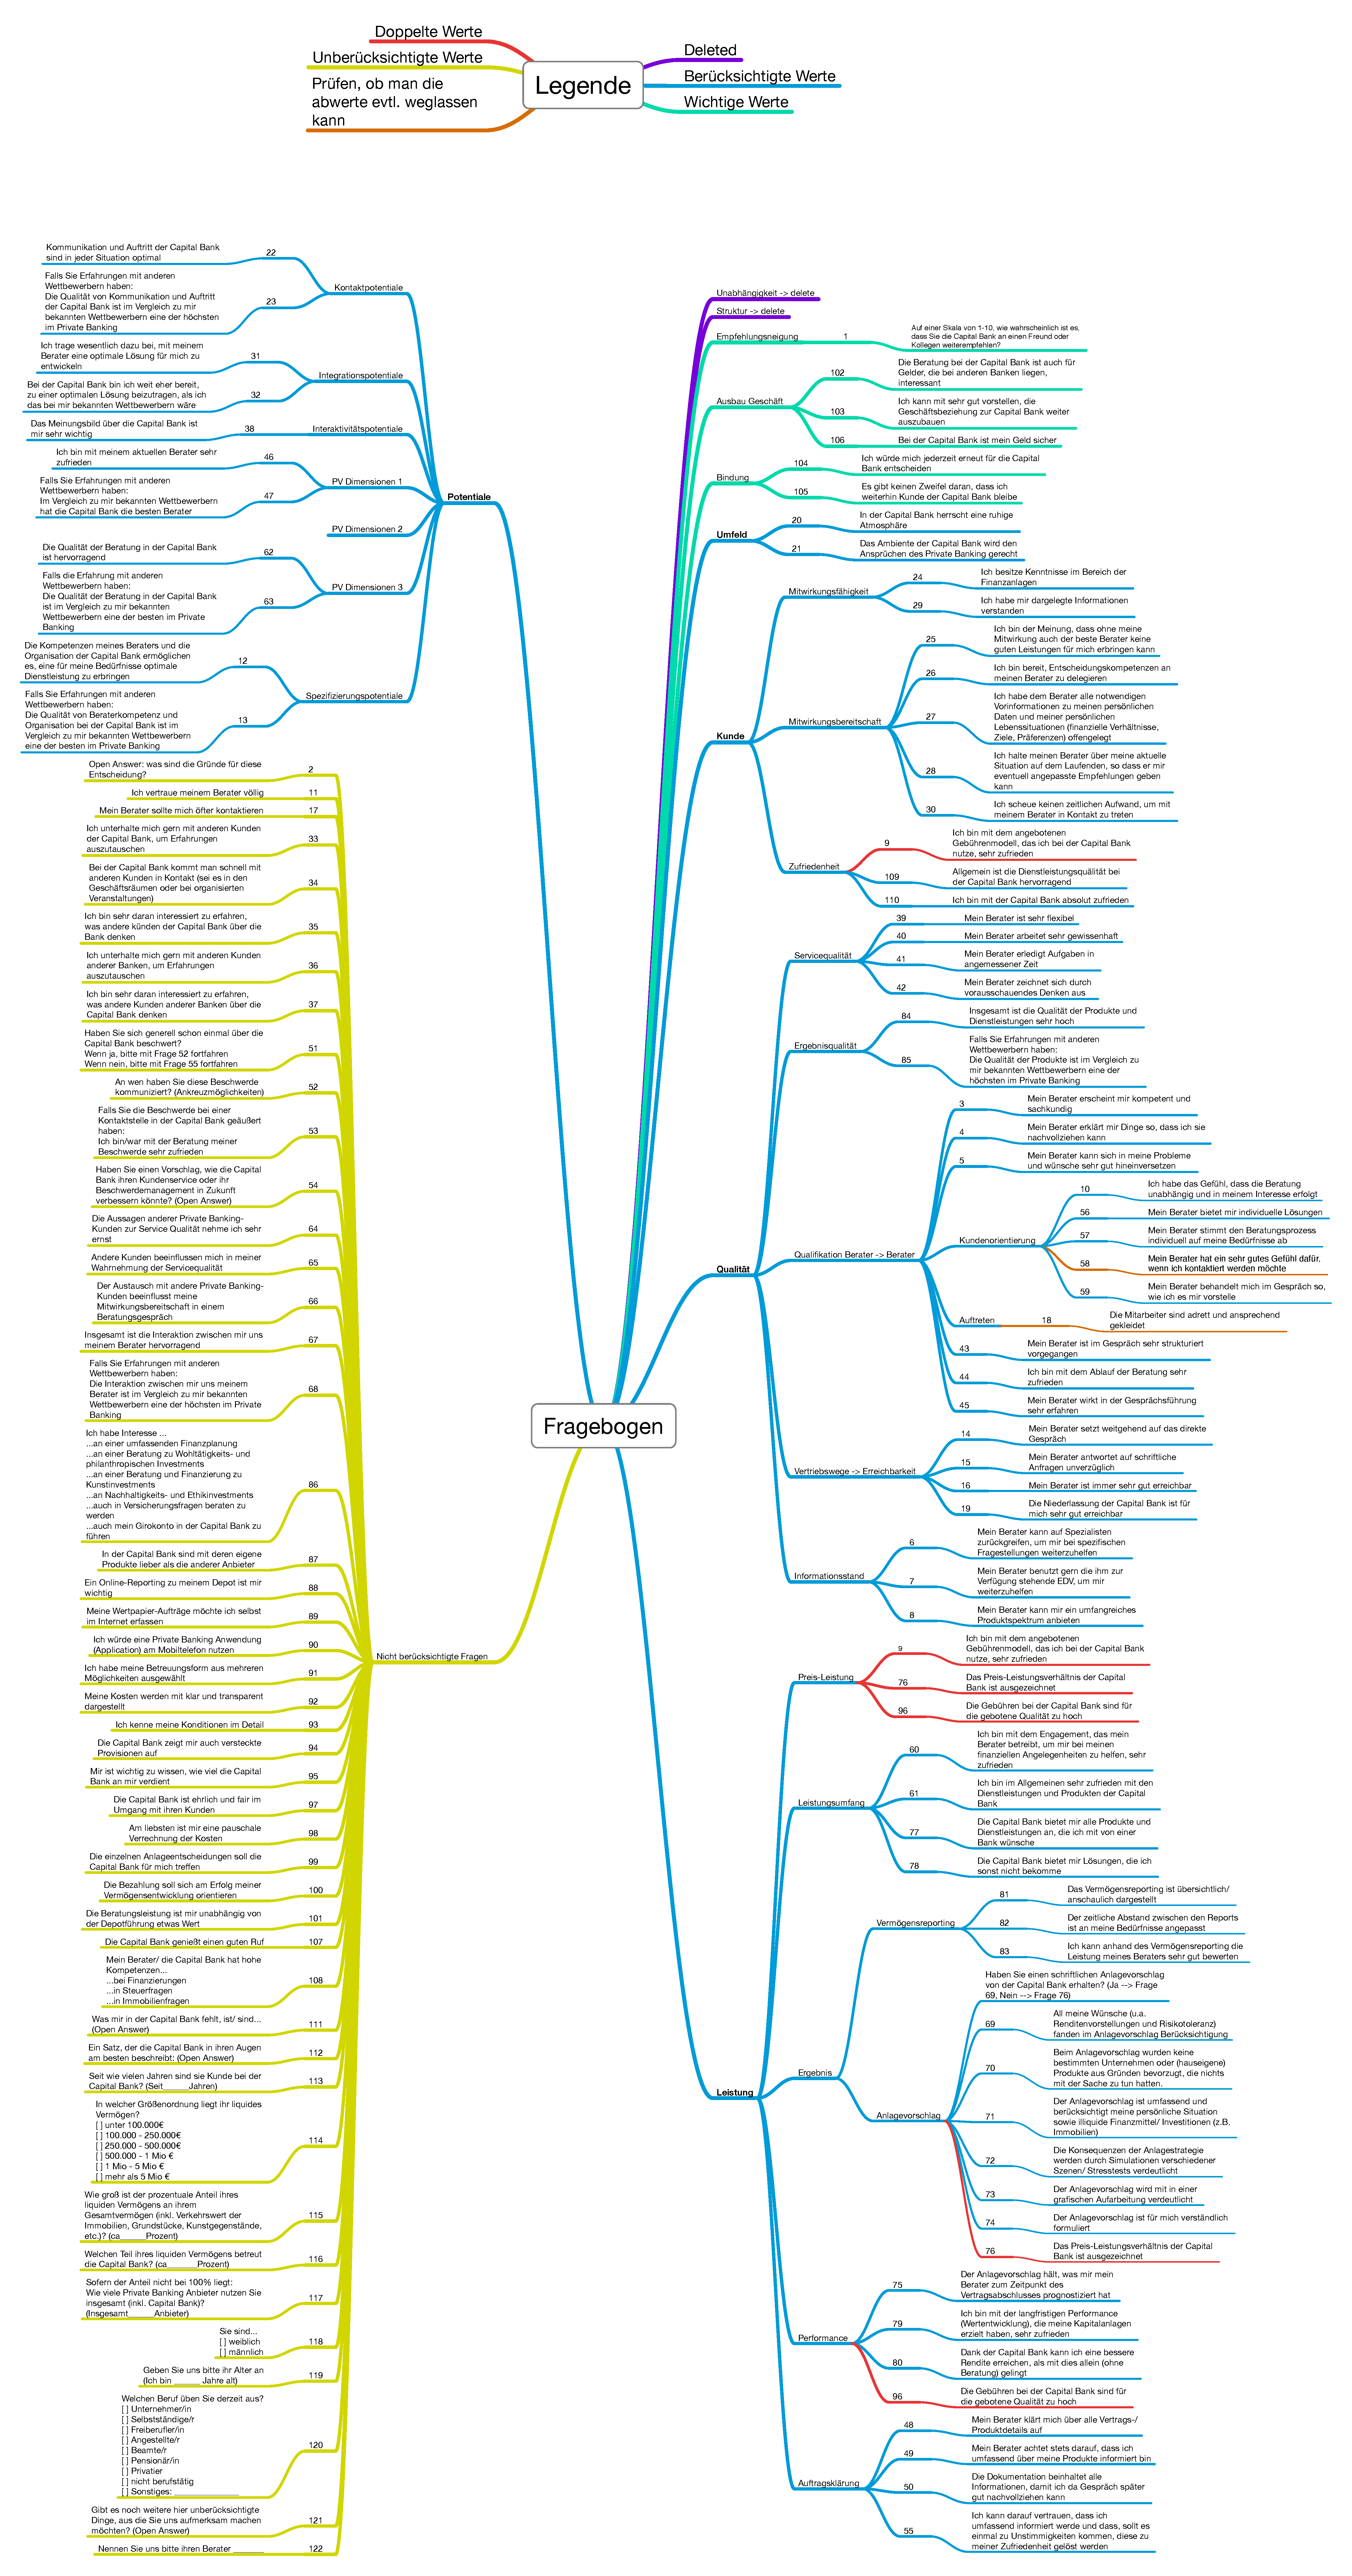
\includepdf[pages={1}]{Grafiken/fragebogen.pdf}
\label{fragebogen}




Unserer Meinung nach wäre es angebracht, eine Kürzung des Fragebogens vorzunehmen. Dazu haben wir im Anschluss durch Berechnungen mit den Programmen R und Smart PLS erfolgreich insgesamt 51 Fragen kürzen können, ohne den Fragebogen in seiner Zielsetzung zu beeinflussen.\\
Die Fragen 3 - 8 und 10, 11, 13 haben wir gekürzt, da es sich um wiederholende, sich auf den Berater beziehende Fragen handelt, deren Aussagekraft im Vergleich weniger aussagekräftig sind. Als Beispiel dazu Frage 12: „Die Kompetenzen meines Beraters und die Organisation der Capital Bank ermöglichen es, eine für meine Bedürfnisse optimale Dienstleistung zu erbringen.“ Die Beantwortung dieser Frage erfolgt schon allein durch die Beantwortung des kompletten Fragebogens, da dieser die Antwort widerspiegelt. Einige Fragen, welche sich in dem Absatz zwischen 35 und 39 befinden sind in ihrer Ordnung sehr unstrukturiert, da sich dort Fragen sowohl zum Kunden als auch zum Berater vermischen und dies eine Unordnung mit sich zieht. Die Frage 35 „Ich bin sehr daran interessiert daran zu erfahren, was andere Kunden der Capital Bank über die Bank denken.“ ist ein gutes Beispiel für sich wiederholende Fragen, da sie der Frage 64 stark ähnelt, welche lautet: „Die Aussagen anderer Private Banking-Kunden zur Service-Qualität nehme ich sehr ernst.“.\\
Ein weiteres Beispiel einer zu empfehlenden Kürzung wäre Frage 86, die mit „Ich habe Interesse…“ beginnt und anschließend Dienstleistungsangebote auflistet. Da der Fragebogen die Dienstleistungsqualität messen soll, erscheint uns in diesem Falle diese Frage unpassend, da unter anderem die drei Zielgrößen Empfehlungsneigung, Kundenbindung und Ergebnisqualität durch die Frage nicht bemessen werden.\\
Wir würden empfehlen, diese in einer eigenen Befragung / Umfrage zu stellen. Genauso wie Frage 86 würden wir die Fragen 88 - 90 ebenfalls selektieren.\\
Die Kompetenz des Beraters und die Kapitalbank spiegelt der Fragebogen im Prinzip wider, weshalb wir die Frage 108 „Mein Berater / Die Capital Bank hat hohe Kompetenzen bei Finanzierungen, in Steuerfragen, in Immobilienfragen.“ als suboptimal erachten.\\
Den Statistikteil 113 - 122 am Ende ist in der Abbildung 2 nicht zu sehen, da diese in dem Modell in SmartPLS nicht erfasst wurden, jedoch sind diese obligatorisch und sollten weiterhin zum Fragebogen hinzugehören.\\
Die Einverständniserklärung am Ende des Fragebogens, in welcher der Kunde sich damit einverstanden erklärt, dass ein Mitarbeiter auf ihn zukommen kann, widerspricht der Anonymitätsgewährleistung zu Beginn des Fragebogens. Dazu würden wir entweder empfehlen, die Anonymität zu gewährleisten und diese Frage nicht zu stellen oder von vornherein darüber zu informieren, dass bei Rückfragen ein Mitarbeiter gegebenenfalls auf den Kunden zukommen kann.\\
Nachdem wir mit Hilfe von Berechnungen und Modellen in SmartPLS und R zu einem abschließenden Entwurf des Fragebogens gekommen sind haben sich folgende Konstrukte ergeben:

\begin{itemize}
\item Kunde
\item Berater
\item Zufriedenheit (aufgegliedert in Ergebnisqualität, Bindung und Empfehlungsneigung)
\item Bank (inklusive Ausbau Geschäft)
\item Mitwirkungsbereitschaft
\item Mitwirkungsfähigkeit
\item Erreichbarkeit
\item Anlagevorschlag
\item Leistungsumfang
\item Umfeld / Umgebung
\item Vermögensreporting
\end{itemize}

Nach der Überarbeitung des Fragebogens beinhaltet dieser nun noch 63 Fragen. Abbildung \ref{fragebogenfertig} zeigt den Fragebogen in Form einer Mindmap nach der Bearbeitung.

%\begin{figure}[h!]
%\centering
%\hspace*{-4.8cm}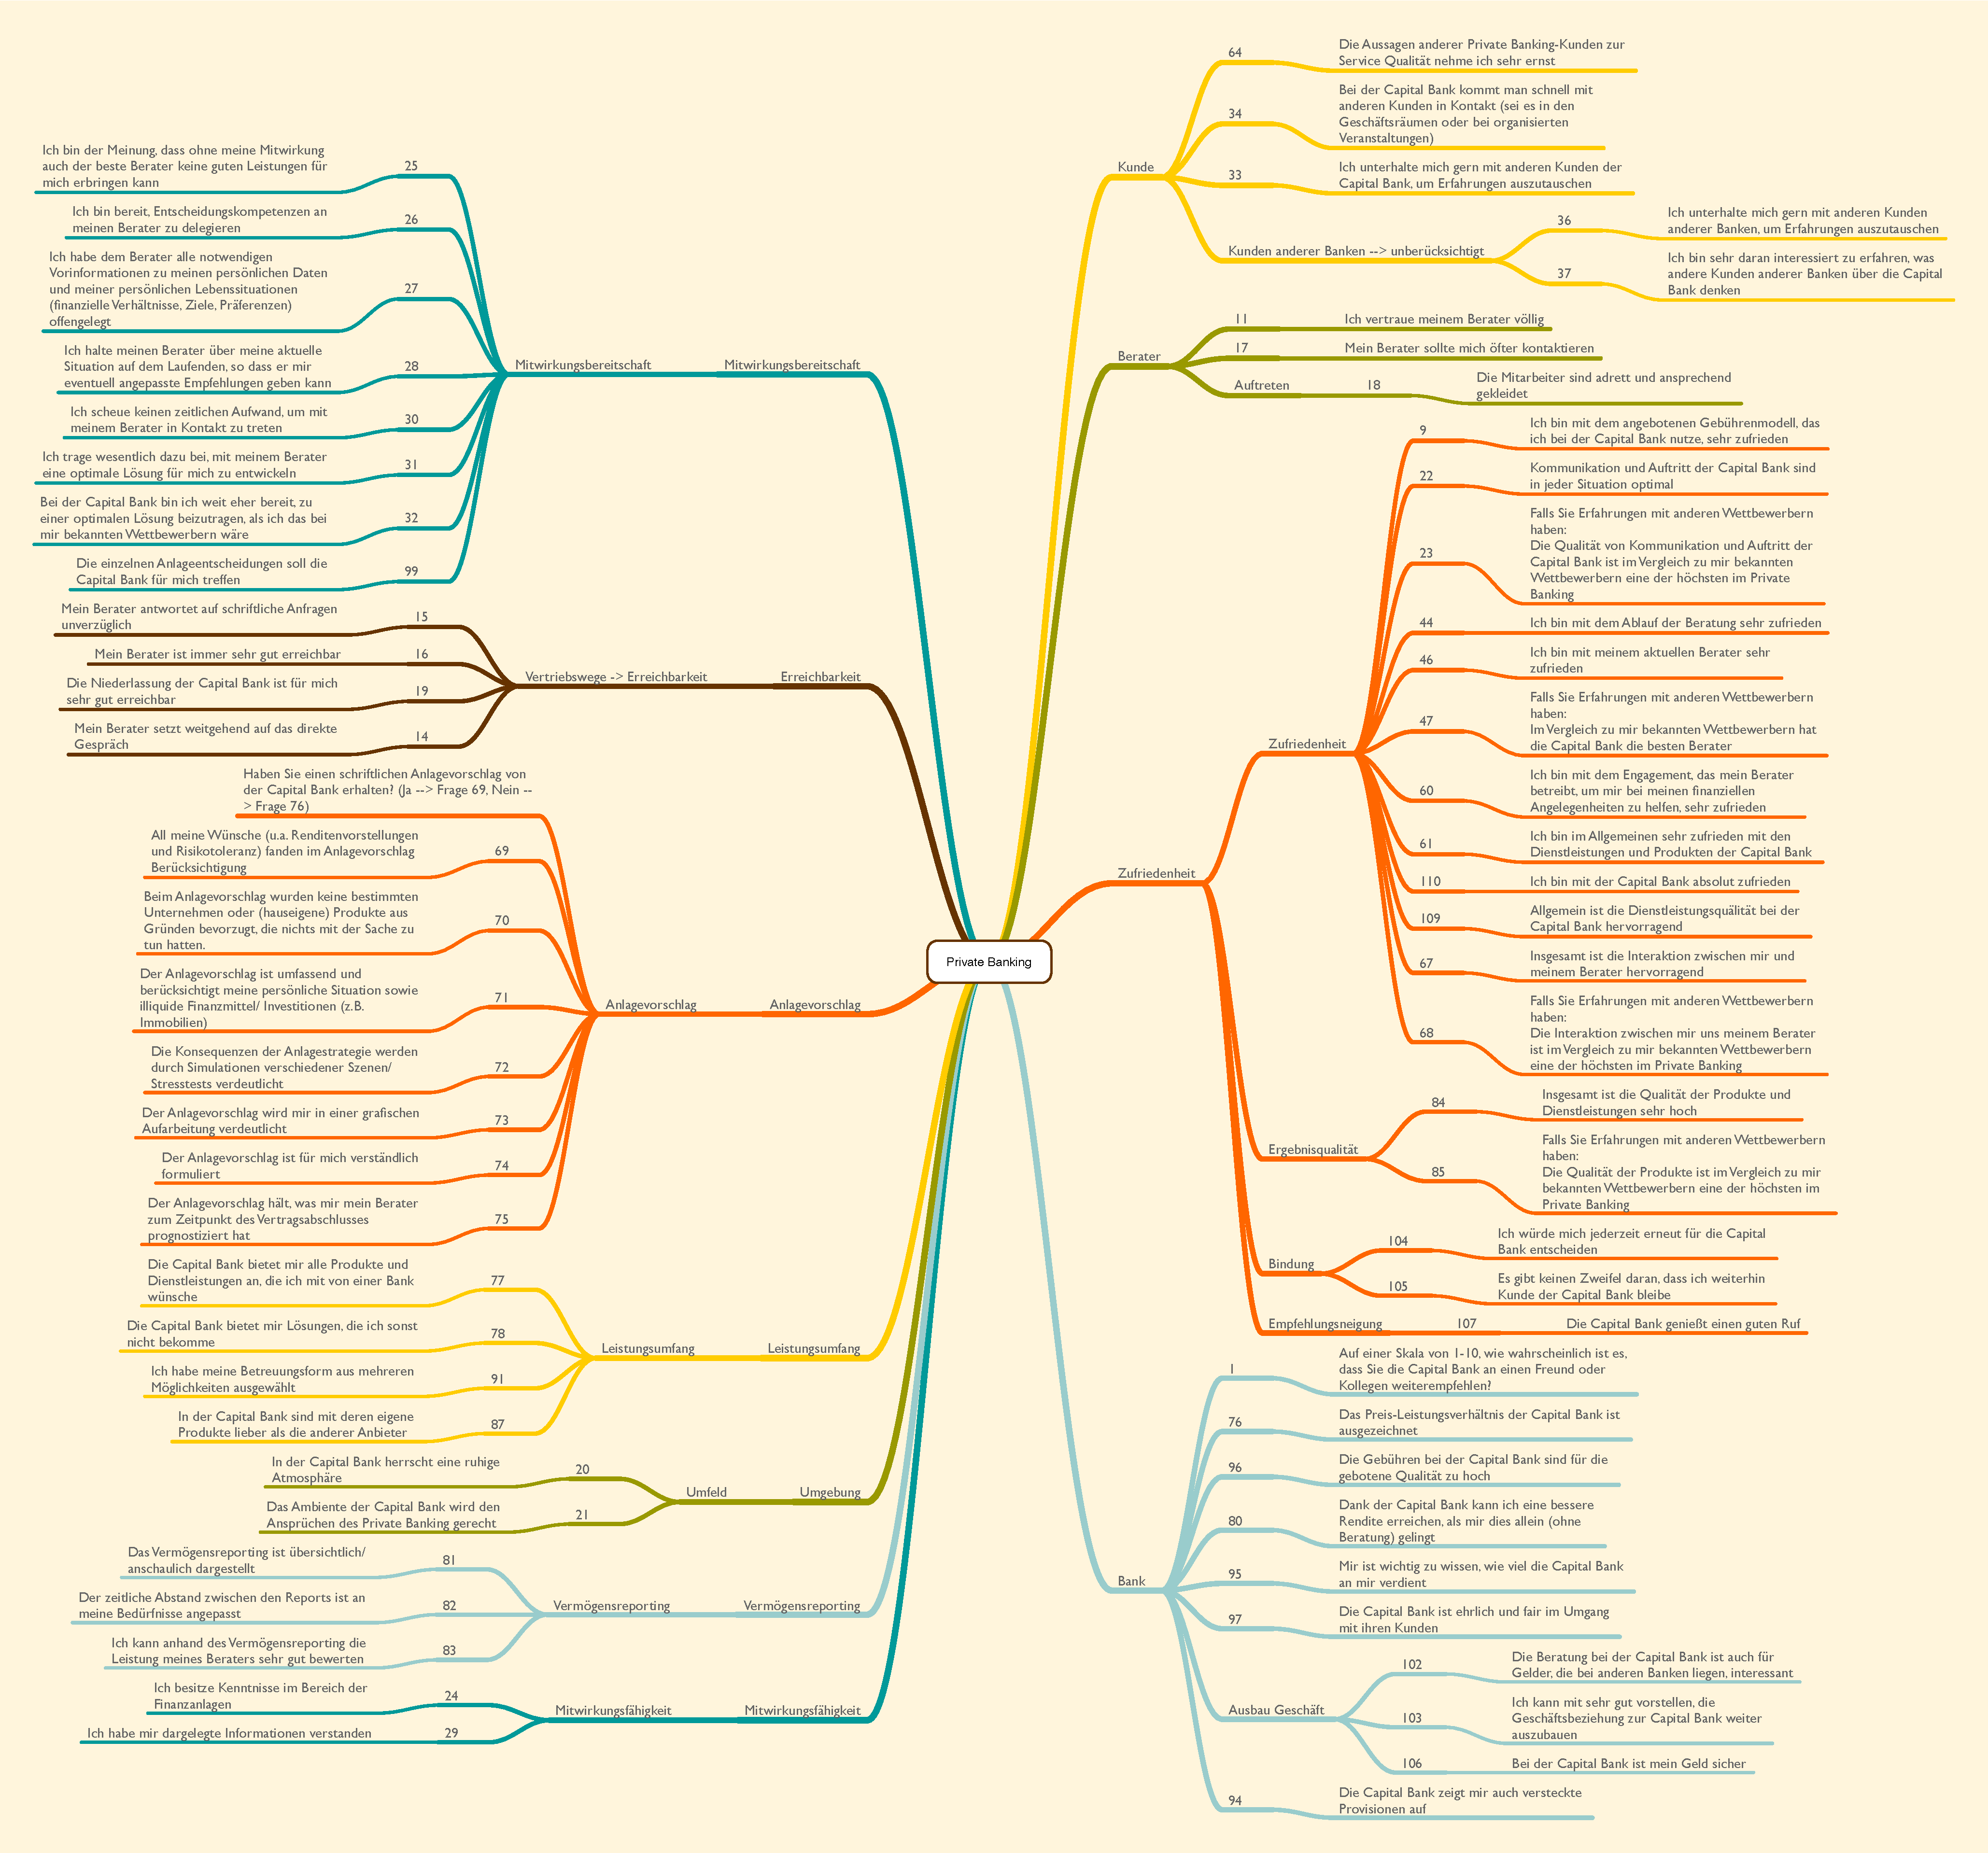
\includegraphics[scale = 0.1]{Grafiken/fragebogenfertig.pdf}
%\caption{Mindmap bearbeiteter Fragebogen}
%\label{fragebogenfertig}
%\end{figure}


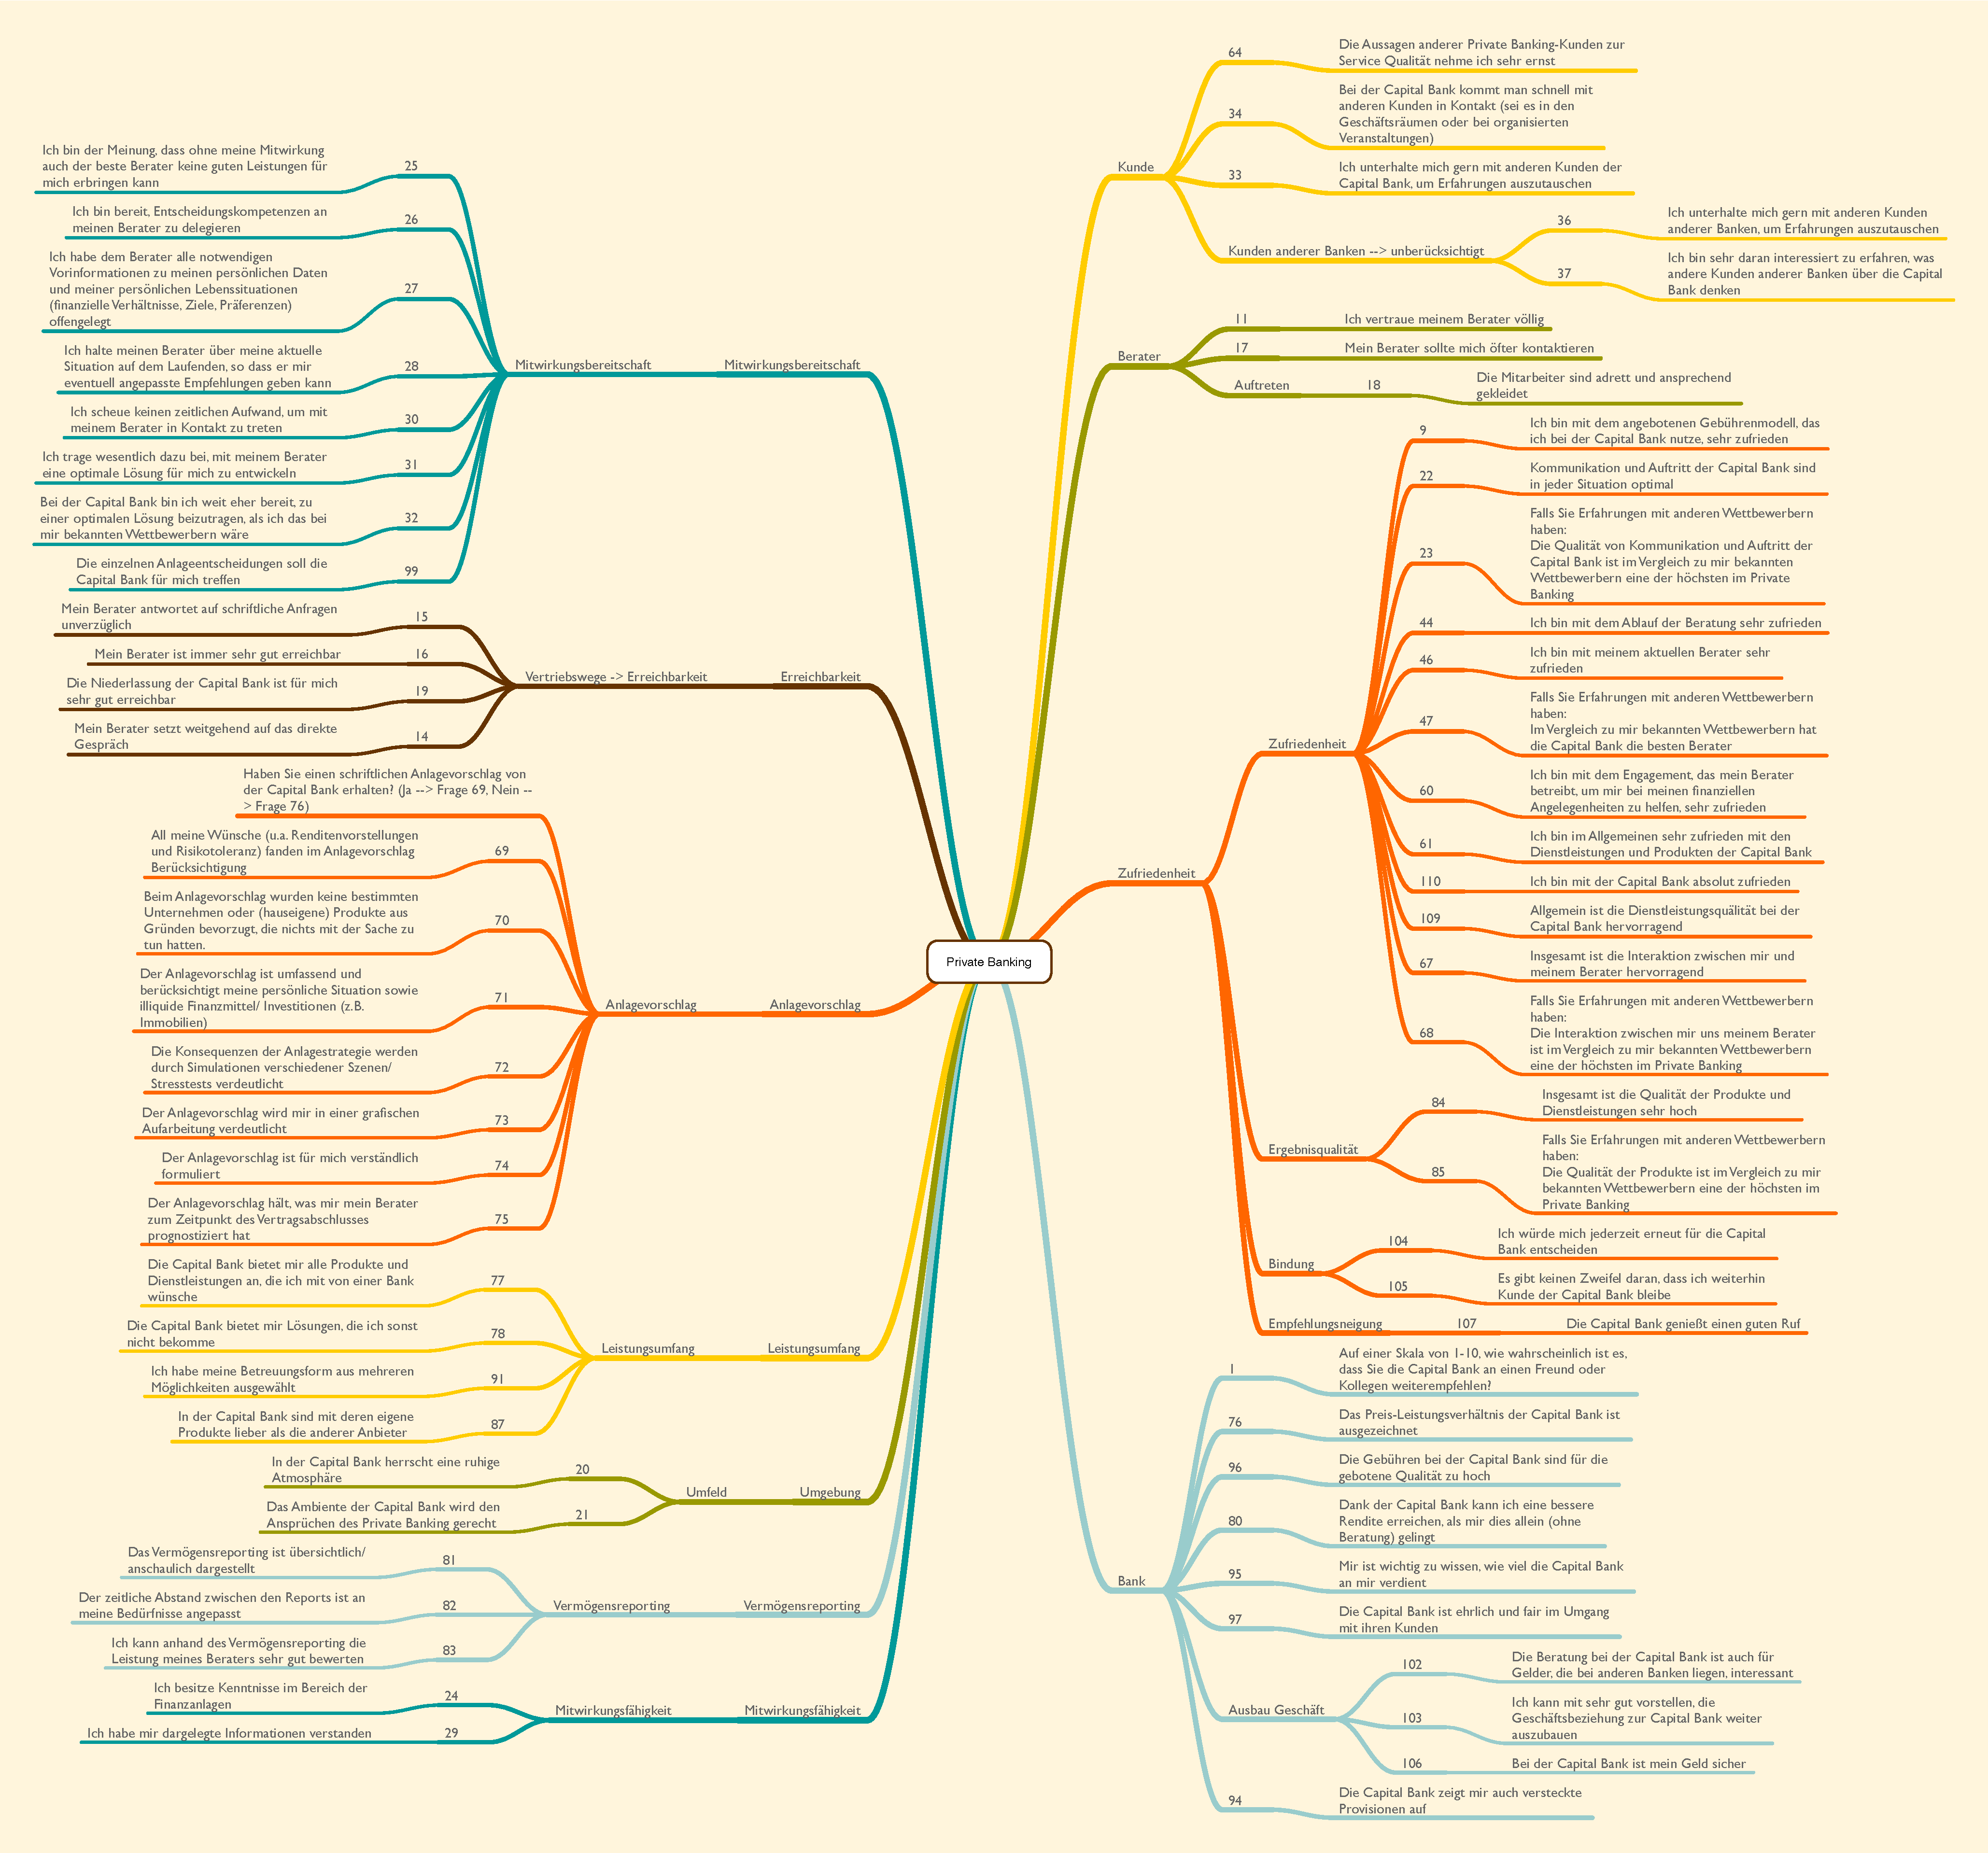
\includepdf[landscape=true]{Grafiken/fragebogenfertig.pdf}
\label{fragebogenfertig}







\section{Software}%Hier soll die benutzte Software vorgestellt werden

\subsection{SmartPLS}

\subsection{R-Pakete}
\href{http://www.r-project.org/}{R} ist eine Programmiersprache und gleichzeitig eine Umgebung zur statistischen Datenverarbeitung, sowie deren Visualisierung. Außerdem ist R ein \href{http://www.gnu.org/}{GNU Projekt} und somit als Open Source Software, unter der \href{http://www.r-project.org/COPYING}{GNU General Public License}, frei verfügbar. Es läuft unter Linux, Windows oder Mac OS X. Eine Erweiterung der Funktionen erfolgt über Pakete, welche von den Usern selbst geschrieben und unter dem \href{http://cran.r-project.org/}{Comprehensive R Archive Network (CRAN)} der Öffentlichkeit zur Verfügung gestellt werden können. Der große Vorteil daran ist dass die jeweiligen Pakete immer weiter verwendet werden können und so eine Art Modularität ensteht. Ein Paket das zur Berechnung von Strukturgleichungsmodellen dient, kann zum Beispiel ein Paket zur graphischen Darstellung von Matrizen verwenden um die Modelle anschaulich zu visualisieren, statt eigens einen neuen Algorithmus dafür schreiben zu müssen. Es empfiehlt sich zusätzlich die Installation einer Integrierten Entwicklungsumgebung, wie beispielsweise \href{http://www.rstudio.com/}{RStudio}. Dies erleichtert die Arbeit durch Funktionen wie die Syntaxhervorhebung, Editor, History, Debugger und Workspace Verwaltung.\\
Nach dem Start von RStudio müssen zunächst die erforderlichen Pakete installiert werden. Dies muss nur einmal ausgeführt und kann daher direkt in die Console eingegeben werden.

\begin{knitrout}
\definecolor{shadecolor}{rgb}{0.969, 0.969, 0.969}\color{fgcolor}\begin{kframe}
\begin{alltt}
\hlkwd{install.packages}\hlstd{(}\hlkwd{c}\hlstd{(}\hlstr{"plspm"}\hlstd{,}\hlstr{"semPLS"}\hlstd{,}\hlstr{"lavaan"}\hlstd{,}\hlstr{"sem"}\hlstd{))}
\hlkwd{source}\hlstd{(}\hlstr{'http://openmx.psyc.virginia.edu/getOpenMx.R'}\hlstd{)}
\end{alltt}
\end{kframe}
\end{knitrout}
Nun wurden alle benötigten Pakete installiert. Anschließend müssen die zur Verwendung geplanten Pakete in die aktuelle R Session geladen werden.

\subsubsection{plspm}
Das Paket plspm\cite{sanchez2013pls} wurde von \href{gaston.stat@gmail.com}{Gaston Sanchez}, Laura Trinchera und Giorgo Russolillo erstellt. Die Webseiten \href{http://gastonsanchez.com}{gastonsanchez.com} und \href{http://www.plsmodeling.com/}{plsmodeling.com} geben Auskunft über weitere Projekte. Außerdem ist für jedes R-Paket ein \href{http://cran.r-project.org/web/packages/plspm/plspm.pdf}{Handbuch} und eine \href{http://cran.r-project.org/web/packages/plspm/vignettes/plspm_introduction.pdf}{Einführung} verfügbar. Eine kurze Dokumentation über einzelne Funktionen ist auch über die Hilfe direkt in R aufrufbar:
\begin{knitrout}
\definecolor{shadecolor}{rgb}{0.969, 0.969, 0.969}\color{fgcolor}\begin{kframe}
\begin{alltt}
\hlcom{#get Help for function plspm()}
\hlkwd{help}\hlstd{(plspm)}

\hlcom{#or}
\hlopt{?}\hlstd{plspm}
\end{alltt}
\end{kframe}
\end{knitrout}
Darauf erscheint in R-Studio ein Hilfe Fenster. Dies kann sehr nützlich sein wenn versucht wird eine Funktion auszuführen ohne zu wissen welche Argumente sie benötigt. Wenn nicht sicher ist welche Funktionen überhaupt im Paket vorhanden sind, kann entweder im oben erwähnten Handbuch nachgeschaut werden oder unter dem Menüpunkt Packages das entsprechende Paket ausgewählt werden.\\
Ein großer Vorteil des plspm Pakets ist die gute Dokumentation. Neben den oben genannten existiert ebenfalls ein frei verfügbares \href{http://www.gastonsanchez.com/PLS Path Modeling with R.pdf}{Buch}\cite{sanchez2013pls}vom Ersteller des Pakets. Außerdem ist das Paket Open Source und der komplette Code ist auf \href{https://github.com/gastonstat/plspm}{Github}verfügbar. Das heißt mit den nötigen Fähigkeiten kann genau nachvollzogen werden wie die Berechnung abläuft und somit Fehler in der Software quasi ausgeschlossen werden.\\
Ein entscheidender Nachteil besteht jedoch in Version 0.4.0 (2013-12-08) bei der Behandlung von fehlenden Werten im Datensatz. Falls auch nur eine einzige Beobachtung bei jedem gemessenen Indikator eines latenten Konstrukts fehlende Werte aufweist, funktioniert der komplette Algorithmus nicht mehr, statt diese eine Beobachtung zu ignorieren. Wenn nun eine latente Variable nur durch einen Indikator gemessen wird, reicht eine Beobachtung welche für diesen Indikator einen fehlenden Wert aufweist um den Algorithmus terminieren zu lassen. Indikatoren sind in unserem Fall die Fragen des Fragebogens und Beobachtungen die Kunden, welche diese beantwortet haben. Da zahlreiche unbeantwortete Fragen im Datensatz existieren, ist also das plspm Paket für unseren Fall nicht brauchbar. Auch die Kontaktaufnahme mit dem Autor half nicht den Fehler zu beseitigen. Eventuell lohnt es sich jedoch die \href{http://cran.r-project.org/web/packages/plspm/NEWS}{Nachrichten}zu neuen Versionen des Pakets zu beobachten. Eine weitere Alternative wäre den frei verfügbaren Code zu manipulieren, wofür jedoch sehr gute R sowie PLS-Algorithmus Kenntnisse von Nöten sind. Nachfolgend wird der R-Code für das Erstellen und Berechnen eines Sturkturmodells mit dem plspm Paket gezeigt. Dafür wurde ein möglichst einfaches, beispielhaftes Modell aus dem Datensatz erstellt um die Übersichtlichkeit und Verständniskeit zu bewahren.

\begin{knitrout}
\definecolor{shadecolor}{rgb}{0.969, 0.969, 0.969}\color{fgcolor}\begin{kframe}
\begin{alltt}
\hlcom{#load package}
\hlkwd{library}\hlstd{(plspm)}

\hlcom{#get filepath}
\hlcom{#CBdataPath <- file.choose()}
\hlstd{CBdataPath} \hlkwb{<-} \hlstr{"/home/jannic/Schreibtisch/PB/Data/2014_08_30-CB_Alle_R.csv"}

\hlcom{#insert data, seperator set to comma, if missing values set to NA}
\hlstd{CBdata} \hlkwb{<-} \hlkwd{read.csv}\hlstd{(CBdataPath,} \hlkwc{sep} \hlstd{=}\hlstr{","}\hlstd{,}\hlkwc{na.strings}\hlstd{=}\hlstr{"NA"}\hlstd{)}

\hlcom{#set missing values to NA}
\hlstd{CBdata[CBdata} \hlopt{==} \hlnum{888}\hlstd{]} \hlkwb{<-} \hlnum{NA}

\hlcom{#specify inner model with lower triangular boolean matrix}
\hlstd{Preis_Leistung} \hlkwb{<-} \hlkwd{c}\hlstd{(}\hlnum{0}\hlstd{,}\hlnum{0}\hlstd{,}\hlnum{0}\hlstd{)}
\hlstd{Performance} \hlkwb{<-} \hlkwd{c}\hlstd{(}\hlnum{0}\hlstd{,}\hlnum{0}\hlstd{,}\hlnum{0}\hlstd{)}
\hlstd{Kundenzufriedenheit} \hlkwb{<-} \hlkwd{c}\hlstd{(}\hlnum{1}\hlstd{,}\hlnum{1}\hlstd{,}\hlnum{0}\hlstd{)}


\hlcom{#create matrix by row binding}
\hlstd{CB_inner_model} \hlkwb{<-} \hlkwd{rbind}\hlstd{(Preis_Leistung,}
                        \hlstd{Performance, Kundenzufriedenheit)}

\hlcom{#add column names }
\hlkwd{colnames}\hlstd{(CB_inner_model)} \hlkwb{<-} \hlkwd{rownames}\hlstd{(CB_inner_model)}

\hlcom{#show inner model}
\hlkwd{innerplot}\hlstd{(CB_inner_model)}
\end{alltt}
\end{kframe}
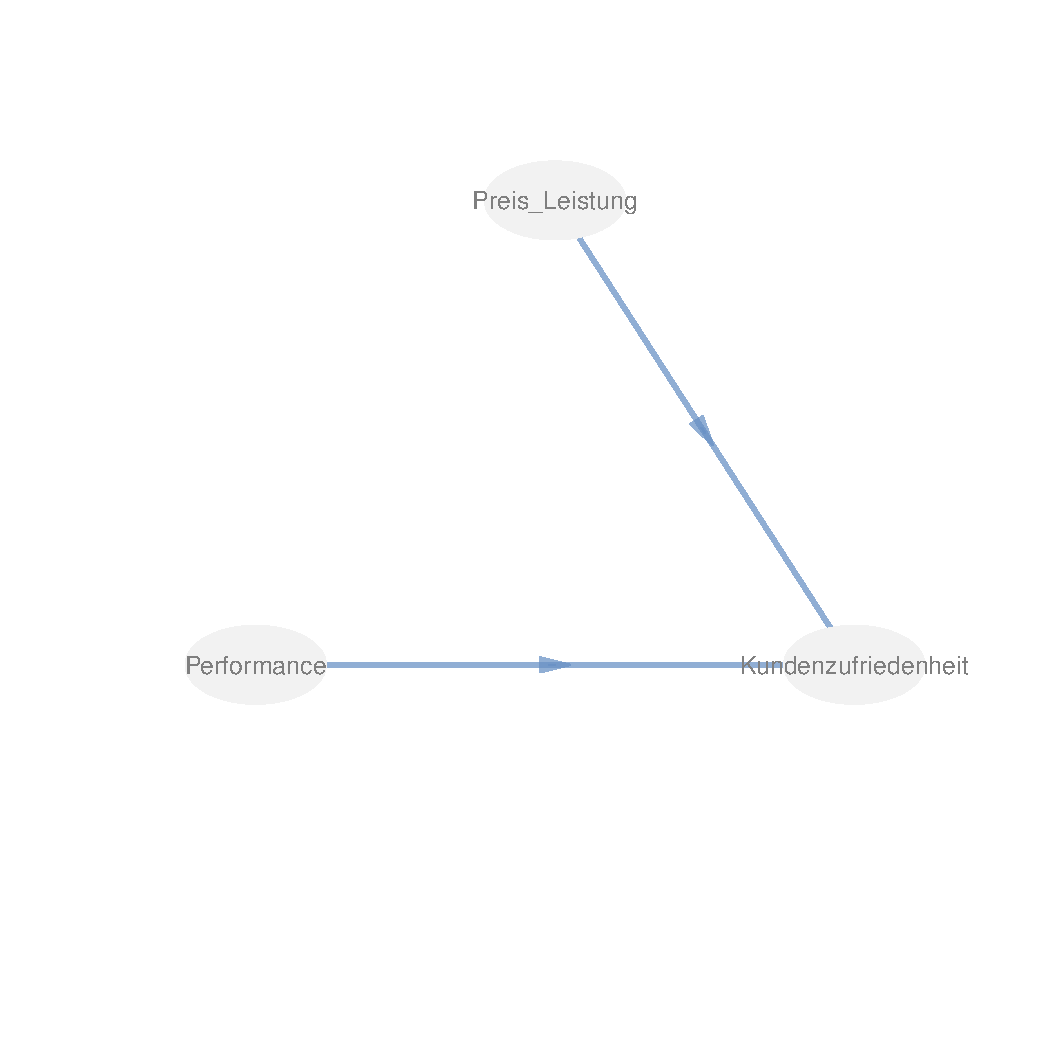
\includegraphics[width=\maxwidth]{figure/plspm} 
\begin{kframe}\begin{alltt}
\hlcom{#specify outer model}
\hlstd{CB_outer_model} \hlkwb{<-} \hlkwd{list}\hlstd{(}\hlkwd{c}\hlstd{(}\hlstr{"SQ060"}\hlstd{,}\hlstr{"SQ062"}\hlstd{,}\hlstr{"SQ096"}\hlstd{,}\hlstr{"SQ076"}\hlstd{),}
                       \hlkwd{c}\hlstd{(}\hlstr{"SQ079"}\hlstd{,}\hlstr{"SQ080"}\hlstd{),}\hlkwd{c}\hlstd{(}\hlstr{"SQ046"}\hlstd{,}\hlstr{"SQ044"}\hlstd{))}

\hlcom{#all variables are measured in a reflective way}
\hlcom{#to measure formative type change character to "B"}
\hlstd{CB_modes} \hlkwb{<-} \hlkwd{c}\hlstd{(}\hlstr{"A"}\hlstd{,}\hlstr{"A"}\hlstd{,}\hlstr{"A"}\hlstd{)}

\hlcom{#set all scaling to numeric}
\hlstd{CB_scaling} \hlkwb{=} \hlkwd{list}\hlstd{(}\hlkwd{c}\hlstd{(}\hlstr{"NUM"}\hlstd{,} \hlstr{"NUM"}\hlstd{,}\hlstr{"NUM"}\hlstd{,} \hlstr{"NUM"}\hlstd{),}
                  \hlkwd{c}\hlstd{(}\hlstr{"NUM"}\hlstd{,} \hlstr{"NUM"}\hlstd{),}
                  \hlkwd{c}\hlstd{(}\hlstr{"NUM"}\hlstd{,} \hlstr{"NUM"}\hlstd{)}
\hlstd{)}

\hlcom{#run plspm function}
\hlstd{CB_PLS} \hlkwb{<-} \hlkwd{plspm}\hlstd{(CBdata,CB_inner_model,CB_outer_model,}
                \hlkwc{modes} \hlstd{= CB_modes,} \hlkwc{scaling} \hlstd{= CB_scaling)}
\end{alltt}


{\ttfamily\noindent\bfseries\color{errorcolor}{\#\# Error: Fehlender Wert, wo TRUE/FALSE nötig ist}}\end{kframe}
\end{knitrout}

\begin{knitrout}
\definecolor{shadecolor}{rgb}{0.969, 0.969, 0.969}\color{fgcolor}\begin{kframe}
\begin{alltt}
\hlkwd{install.packages}\hlstd{(}\hlstr{"zoo"}\hlstd{)}
\end{alltt}
\end{kframe}
\end{knitrout}

\begin{knitrout}
\definecolor{shadecolor}{rgb}{0.969, 0.969, 0.969}\color{fgcolor}\begin{kframe}
\begin{alltt}
\hlcom{#load zoo package}
\hlkwd{library}\hlstd{(zoo)}

\hlcom{#interpolate missing values}
\hlstd{CBdata_new} \hlkwb{<-} \hlstd{CBdata}
\hlstd{idx} \hlkwb{<-} \hlkwd{colSums}\hlstd{(}\hlopt{!}\hlkwd{is.na}\hlstd{(CBdata))} \hlopt{>} \hlnum{1}
\hlstd{CBdata_new[ , idx]} \hlkwb{<-} \hlkwd{round}\hlstd{(}\hlkwd{na.approx}\hlstd{(CBdata_new[ , idx]))}
\hlstd{CBdata_new} \hlkwb{<-} \hlstd{CBdata_new[}\hlopt{-}\hlnum{261}\hlstd{,]}

\hlcom{#run plspm function with interpolated dataset}
\hlstd{CB_PLS} \hlkwb{<-} \hlkwd{plspm}\hlstd{(CBdata_new,CB_inner_model,CB_outer_model,}
                \hlkwc{modes} \hlstd{= CB_modes,} \hlkwc{scaling} \hlstd{= CB_scaling)}

\hlcom{#get a summary of the estimated model}
\hlkwd{summary}\hlstd{(CB_PLS)}
\end{alltt}
\begin{verbatim}
## PARTIAL LEAST SQUARES PATH MODELING (PLS-PM) 
## 
## ---------------------------------------------------------- 
## MODEL SPECIFICATION 
## 1   Number of Cases      260 
## 2   Latent Variables     3 
## 3   Manifest Variables   8 
## 4   Scale of Data        Standardized Data 
## 5   Non-Metric PLS       TRUE 
## 6   Weighting Scheme     centroid 
## 7   Tolerance Crit       1e-06 
## 8   Max Num Iters        100 
## 9   Convergence Iters    4 
## 10  Bootstrapping        FALSE 
## 11  Bootstrap samples    NULL 
## 
## ---------------------------------------------------------- 
## BLOCKS DEFINITION 
##                   Block         Type   Size   Mode
## 1        Preis_Leistung    Exogenous      4      A
## 2           Performance    Exogenous      2      A
## 3   Kundenzufriedenheit   Endogenous      2      A
## 
## ---------------------------------------------------------- 
## BLOCKS UNIDIMENSIONALITY 
##                      Mode  MVs  C.alpha  DG.rho  eig.1st  eig.2nd
## Preis_Leistung          A    4    0.387   0.659     2.09    1.049
## Performance             A    2    0.780   0.901     1.64    0.360
## Kundenzufriedenheit     A    2    0.880   0.943     1.78    0.215
## 
## ---------------------------------------------------------- 
## OUTER MODEL 
##                       weight  loading  communality  redundancy
## Preis_Leistung                                                
##   1 SQ060             0.5121    0.888       0.7881       0.000
##   1 SQ062             0.4684    0.881       0.7755       0.000
##   1 SQ096            -0.0253   -0.220       0.0482       0.000
##   1 SQ076             0.2057    0.620       0.3839       0.000
## Performance                                                   
##   2 SQ079             0.4752    0.876       0.7678       0.000
##   2 SQ080             0.6269    0.931       0.8666       0.000
## Kundenzufriedenheit                                           
##   3 SQ046             0.4963    0.937       0.8788       0.490
##   3 SQ044             0.5619    0.952       0.9054       0.505
## 
## ---------------------------------------------------------- 
## CROSSLOADINGS 
##                      Preis_Leistung  Performance  Kundenzufriedenheit
## Preis_Leistung                                                       
##   1 SQ060                     0.888        0.403                0.728
##   1 SQ062                     0.881        0.476                0.666
##   1 SQ096                    -0.220       -0.183               -0.036
##   1 SQ076                     0.620        0.398                0.292
## Performance                                                          
##   2 SQ079                     0.445        0.876                0.263
##   2 SQ080                     0.486        0.931                0.347
## Kundenzufriedenheit                                                  
##   3 SQ046                     0.671        0.290                0.937
##   3 SQ044                     0.734        0.354                0.952
## 
## ---------------------------------------------------------- 
## INNER MODEL 
## $Kundenzufriedenheit
##                   Estimate   Std. Error     t value   Pr(>|t|)
## Intercept        -4.07e-16       0.0415   -9.82e-15   1.00e+00
## Preis_Leistung    7.75e-01       0.0484    1.60e+01   1.86e-40
## Performance      -5.69e-02       0.0484   -1.18e+00   2.41e-01
## 
## ---------------------------------------------------------- 
## CORRELATIONS BETWEEN LVs 
##                      Preis_Leistung  Performance  Kundenzufriedenheit
## Preis_Leistung                1.000        0.516                0.745
## Performance                   0.516        1.000                0.343
## Kundenzufriedenheit           0.745        0.343                1.000
## 
## ---------------------------------------------------------- 
## SUMMARY INNER MODEL 
##                            Type     R2  Block_Communality  Mean_Redundancy
## Preis_Leistung        Exogenous  0.000              0.499            0.000
## Performance           Exogenous  0.000              0.817            0.000
## Kundenzufriedenheit  Endogenous  0.558              0.892            0.498
##                        AVE
## Preis_Leistung       0.499
## Performance          0.817
## Kundenzufriedenheit  0.892
## 
## ---------------------------------------------------------- 
## GOODNESS-OF-FIT 
## [1]  0.6144
## 
## ---------------------------------------------------------- 
## TOTAL EFFECTS 
##                            relationships   direct  indirect    total
## 1          Preis_Leistung -> Performance   0.0000         0   0.0000
## 2  Preis_Leistung -> Kundenzufriedenheit   0.7746         0   0.7746
## 3     Performance -> Kundenzufriedenheit  -0.0569         0  -0.0569
\end{verbatim}
\begin{alltt}
\hlcom{#plot the model}
\hlkwd{plot}\hlstd{(CB_PLS)}
\end{alltt}
\end{kframe}
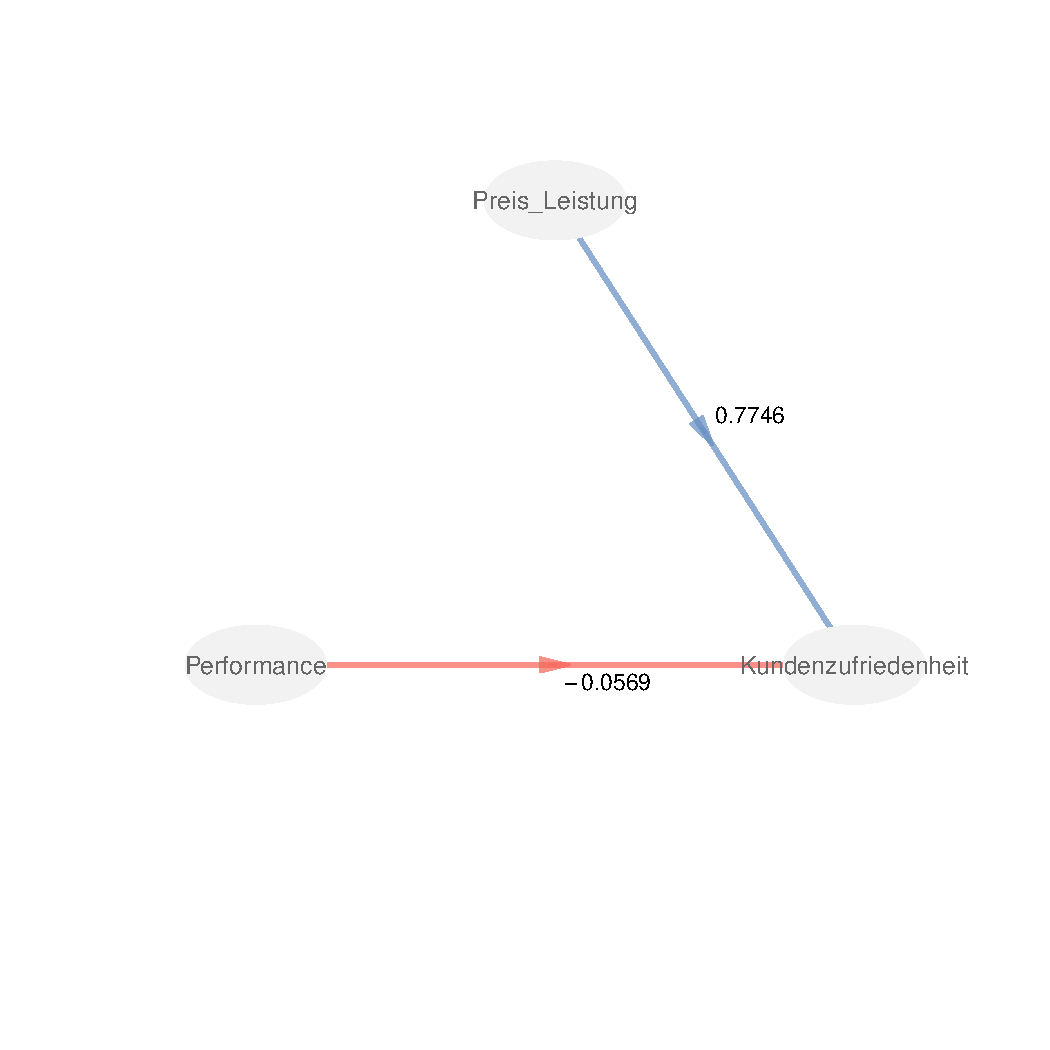
\includegraphics[width=\maxwidth]{figure/zoo1} 
\begin{kframe}\begin{alltt}
\hlcom{#plot the outer model}
\hlkwd{outerplot}\hlstd{(CB_PLS)}
\end{alltt}
\end{kframe}
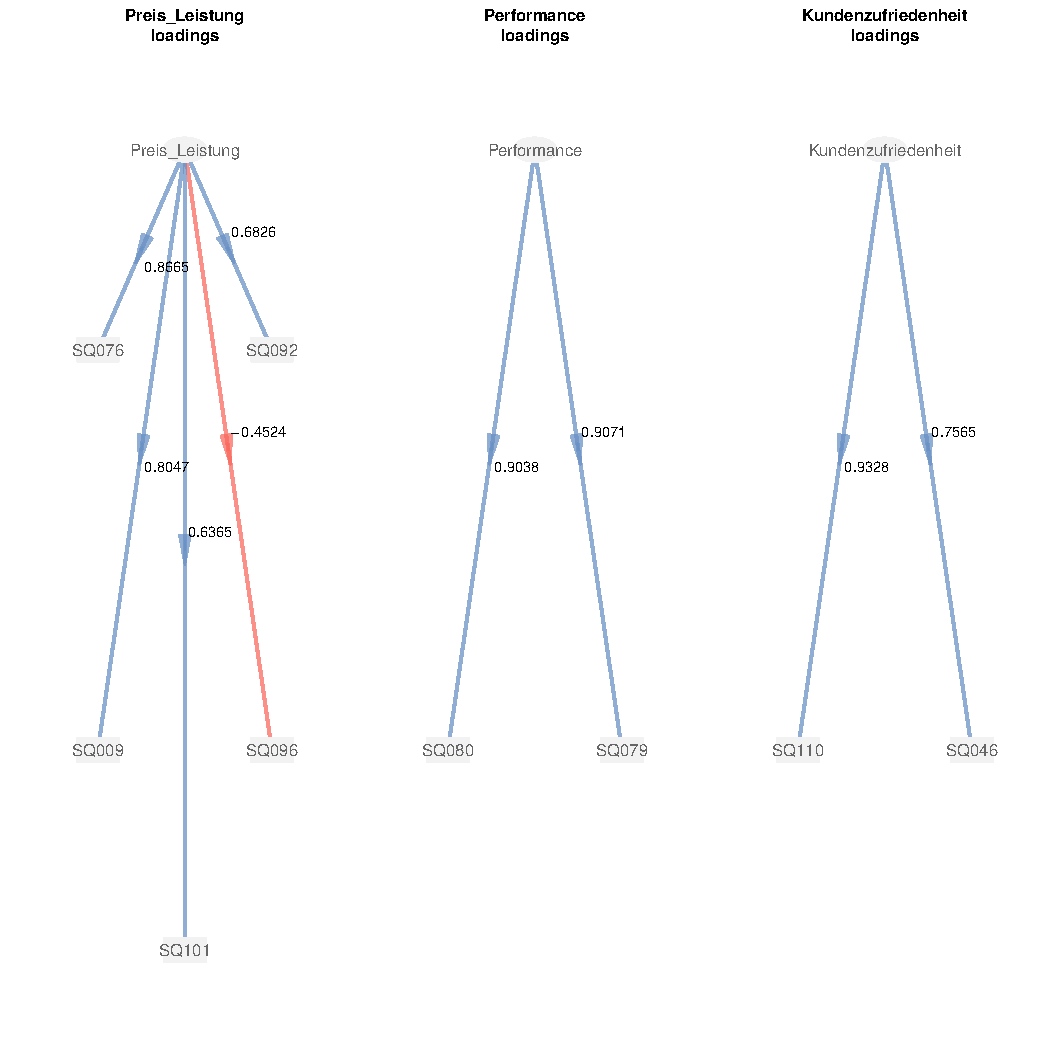
\includegraphics[width=\maxwidth]{figure/zoo2} 

\end{knitrout}

Beschreibung zum Code:\\
Zunächst wird das Paket in die aktuelle R-Session geladen. Als nächstes wird ein Datensatz benötigt. Durch den file.choose() Befehl kann im Verzeichnis des Computers durch die Ordner zum gewünschten Datensatz navigiert werden. Wird dieser nun ausgewählt ist der Verzeichnispfad erst einmal in der Variable CBdataPath gespeichert. In R-Studio wird nun unter "Environment" diese Variable und ihr Wert angezeigt. Um die Datei jedoch einzulesen wird die Funktion read.csv() oder alternativ read.table() benötigt. Als Argument bekommt diese den vorher ausgewählten Dateipfad, welcher in der Variable CBdataPath gespeichert ist. Alternativ kann natürlich auch direkt der Dateipfad in Form eines Strings oder die Funktion file.choose() als Argument eingefügt werden. Auch wenn solche Abkürzungen den Code erheblich komprimieren sollte auch immer auf eine Lesbarkeit geachtet werden damit er auch für neue Nutzer verständlich bleibt. Falls fehlenden Werte als leere Felder dargestellt werden, können diese durch einen weiteren Parameter der read.csv() Funktion na.strings = "NA" auf die R-Standardnotation "NA" gesetzt werden . Falls der Datensatz Fehlende Werte als 888 darstellt, wie in smartPLS werden diese durch einen neuen Befehl (siehe Code) in "NA" umgewandelt. Falls die Spalten im Datensatz durch Semikolon getrennt werden kann entweder die Funktion read.csv2() benutzt werden oder ein weiterer Parameter in die read.csv() Funktion übergeben werden (sep=";"). Nun sehen wir unsere nächste Variable CBdata unter "Environment". Dies ist nun unser Datensatz welcher auch durch einen Klick auf das Tabellenzeichen angeschaut werden kann. Als nächstes wird das Strukturmodell (inneres Modell) definiert. Dies geschieht durch das Erstellen einer unteren Dreiecksmatrix. Zunächst wird also für jede Latente Variable im Modell ein Vektor erstellt mit der Länge der Gesamtzahl der Latenten Variablen und den Werten 0 oder 1. Eins bedeutet hier eine Verbindung und Null dementsprechend keine. Die Richtung des Zusammenhangs wird wie folgt gelesen: Von Spalte, zu Zeile. Zur besseren Lesbarkeit werden die Zeilennamen der Matrix gleich den Spaltennamen gesetzt. Nun können durch einen Klick auf das Tabellensymbol neben der CB\_inner\_model Variable im Environment die Beziehungen abgelesen werden. Die Diagonale besteht nur aus Nullen, da sonst eine Variable sich selbst erklären würde. Ebenso besteht der Teil über der Diagonale, die obere Matrix aus Nullen, damit keine Schleifen entstehen können was im PLS-Algorithmus ebenfalls nicht erlaubt ist. Allerdings erschwert dies die Spezifikation von Modellen, da es sein kann dass im Model keine Schleifen sind, obwohl in der oberen Matrix eine 1 steht. Dies muss nun behoben werden durch vertauschen der Spalten damit die 1 unterhalb der Matrix steht.
\begin{knitrout}
\definecolor{shadecolor}{rgb}{0.969, 0.969, 0.969}\color{fgcolor}\begin{kframe}
\begin{alltt}
\hlcom{#does not work}
\hlstd{Preis_Leistung} \hlkwb{<-} \hlkwd{c}\hlstd{(}\hlnum{0}\hlstd{,}\hlnum{0}\hlstd{,}\hlnum{0}\hlstd{)}
\hlstd{Performance} \hlkwb{<-} \hlkwd{c}\hlstd{(}\hlnum{1}\hlstd{,}\hlnum{0}\hlstd{,}\hlnum{1}\hlstd{)}
\hlstd{Kundenzufriedenheit} \hlkwb{<-} \hlkwd{c}\hlstd{(}\hlnum{1}\hlstd{,}\hlnum{0}\hlstd{,}\hlnum{0}\hlstd{)}

\hlstd{CB_inner_model} \hlkwb{<-} \hlkwd{rbind}\hlstd{(Preis_Leistung,}
                        \hlstd{Performance, Kundenzufriedenheit)}

\hlkwd{innerplot}\hlstd{(CB_inner_model,} \hlkwc{main}\hlstd{=}\hlstr{"SEM: valid, plspm: not valid"}\hlstd{)}
\end{alltt}
\end{kframe}
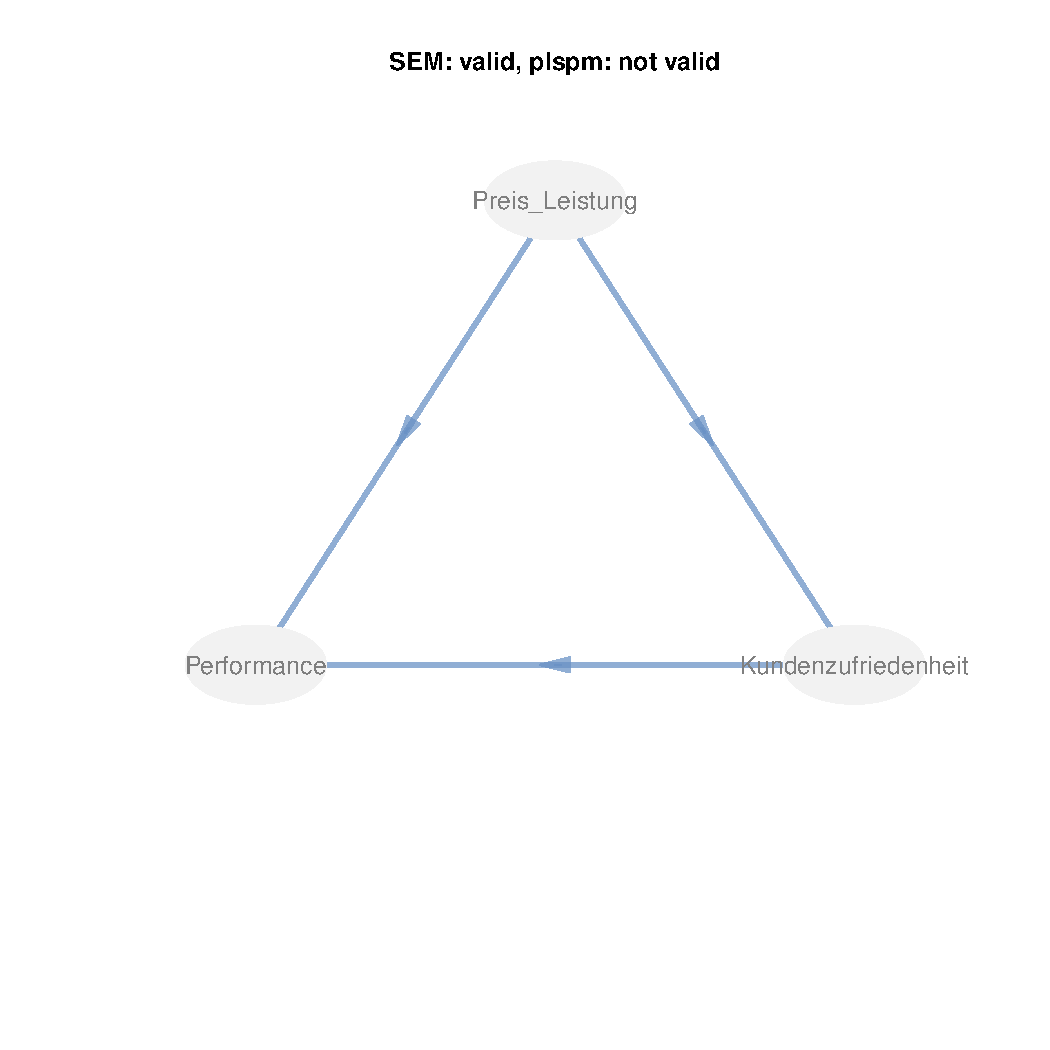
\includegraphics[width=\maxwidth]{figure/mis1} 
\begin{kframe}\begin{alltt}
\hlcom{#works}
\hlstd{Preis_Leistung} \hlkwb{<-} \hlkwd{c}\hlstd{(}\hlnum{0}\hlstd{,}\hlnum{0}\hlstd{,}\hlnum{0}\hlstd{)}
\hlstd{Kundenzufriedenheit} \hlkwb{<-} \hlkwd{c}\hlstd{(}\hlnum{1}\hlstd{,}\hlnum{0}\hlstd{,}\hlnum{0}\hlstd{)}
\hlstd{Performance} \hlkwb{<-} \hlkwd{c}\hlstd{(}\hlnum{1}\hlstd{,}\hlnum{1}\hlstd{,}\hlnum{0}\hlstd{)}

\hlstd{CB_inner_model} \hlkwb{<-} \hlkwd{rbind}\hlstd{(Preis_Leistung,}
                        \hlstd{Kundenzufriedenheit, Performance)}

\hlkwd{innerplot}\hlstd{(CB_inner_model,} \hlkwc{main}\hlstd{=}\hlstr{"SEM: valid, plspm: valid"}\hlstd{)}
\end{alltt}
\end{kframe}
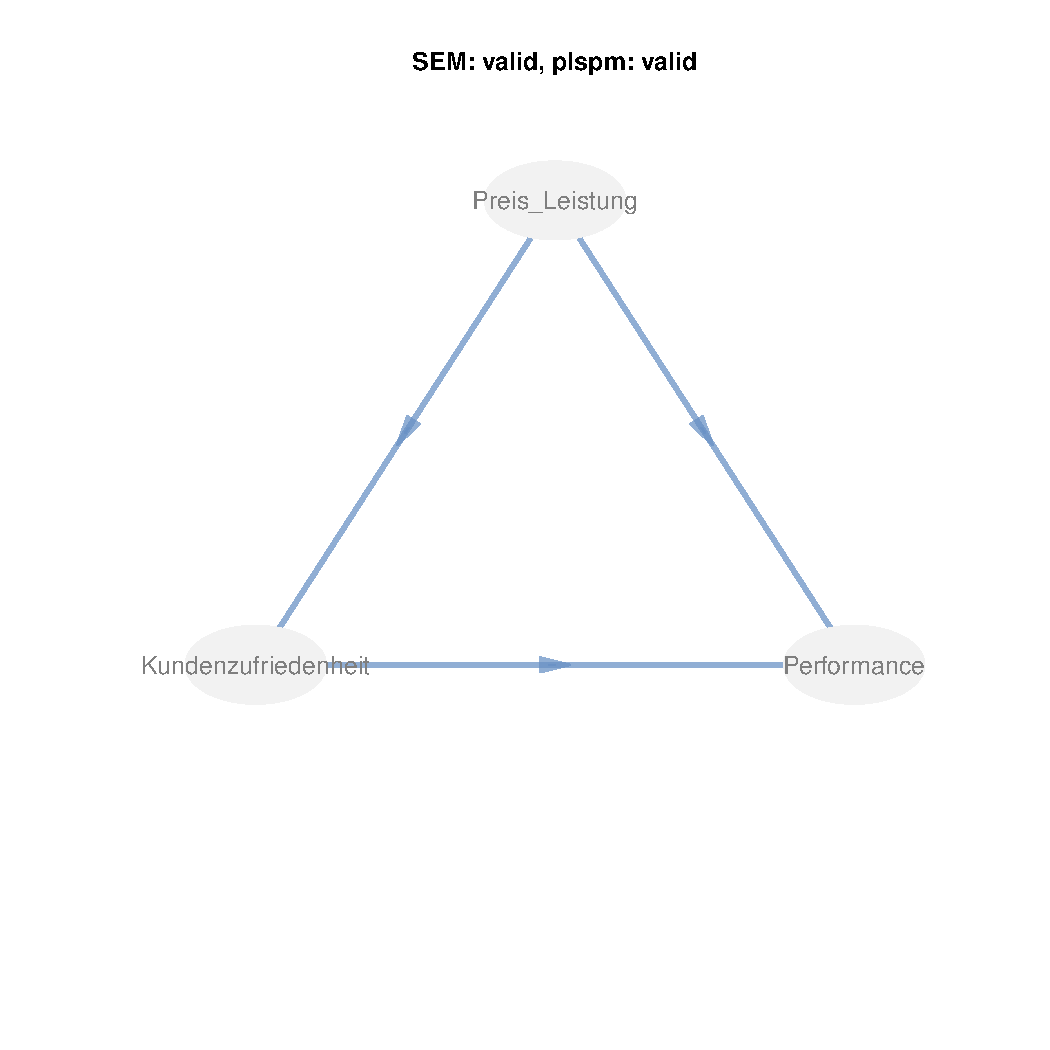
\includegraphics[width=\maxwidth]{figure/mis2} 

\end{knitrout}
Um sicher zu gehen ob das gewünschte Modell spezifiziert wurde kann durch den Befehl innerplot() eine graphische Veranschaulichung aufgerufen werden, welche im Plots Tab erscheint. Das vertauschen der Spalten, beeinflusst auch das Messmodell (äußeres Modell), welches durch eine Liste von Vektoren spezifiziert wird. Hier sind die Vektoren die Latenten Variablen in der Reihenfolge des rbind() Befehls und der Inhalt der Vektoren die Indikatoren eines Konstrukts. Anschließend muss noch ein Vektor erstellt werden, welcher die Messmethode für jedes Konstrukt enthält. Der Buchstabe "A" repräsentiert die reflektive Messung und "B" dementsprechend eine formative Messung.\\
Nun sind alle Parameter für die Hauptfunktion plspm() verfügbar. Diese ist zur Berechnung des Modells zuständig und bekommt in ihrer einfachsten Form folgende Parameter:\\
\begin{enumerate}
    \item Datensatz
    \item Sturkturmodell
    \item Messmodell
    \item Messmethoden
\end{enumerate}
Für das Behandeln von fehlenden Werten muss ein weiterer Parameter übergeben werden. Der scaling Parameter gibt die Skalierung der Indikatoren an. Für eine Berechnung mit fehlenden Werten müssen diese auf "NUM" für Numerisch gesetzt werden. Allerdings bleibt das weiter oben beschriebene Problem bei einer Beobachtung, für die alle Werte der Indikatoren einer Latente Variable fehlen, weiter bestehen. Diese müssten also mit viel Aufwand per Hand entfernt werden, was vor allem bei regelmäßiger Veränderung des Modells ausartet. Wird die Funktion nun ausgeführt entsteht der bereits weiter oben erwähnte Fehler und das Modell kann nicht berechnet werden.\\
Zur Demonstration der Ergebnisse wurden die fehlenden Werte mit dem zoo Paket interpoliert um somit den Fehler zu beheben. Der Code zur Interpolation soll hier nicht weiter erläutert werden. In der Variable CB\_PLS sind nun die Ergebnisse der plspm Funktion gespeichert. Durch den summary() Befehl können diese nun in der Console ausgegeben werden. Dazu kann das Strukturmodell auch durch die plot() Funktion und das Messmodell durch outerplot() visualisiert werden. In den Plots sind nun neben den Konstrukten und Indikatoren auch die jeweiligen Pfadkoeffizienten zu sehen.

\subsubsection{semPLS}
Das Paket semPLS\cite{semPLS} wurde von \href{Armin.Monecke@stat.uni-muenchen.de}{Armin Monecke} und \href{Friedrich.Leisch@R-project.org}{Friedrich Leisch} geschrieben. Wie bei jedem Paket finden sich hierzu ein \href{http://cran.r-project.org/web/packages/semPLS/semPLS.pdf}{Handbuch} und eine kurze \href{http://cran.r-project.org/web/packages/semPLS/vignettes/semPLS-intro.pdf}{Einführung}.\\
Das Paket erwies sich nach Meinung der Autoren als derzeit bestes für Strukturgleichungsmodelle basierend auf dem PLS Ansatz. Einziger Nachteil des Pakets ist die eher umständliche Visualisierung der Modelle mit dot - \href{http://www.graphviz.org/}{Graphviz}. Besonders nützlich ist das einfache importieren von Modellen die in SmartPLS erstellt wurden. Somit können die Vorteile von SmartPLS, einfache Modellierung per Drag \& Drop und die von R, mehr Funktionalitäten, kombiniert werden. Ein weiterer Vorteil könnte auch das Umwandeln des Modells in ein Objekt, welches Kovarianz basierte Berechnungen mit Hilfe des sem Pakets von \href{jfox@mcmaster.ca}{John Fox} erlaubt. Dies könnte sich vor allem in kommenden Praktika als nützlich erweisen um bei einem größeren Datensatz, einem weiter entwickelten Modell und mehr Erfahrung, den eher bestätigenden Kovarianzbasierten Ansatz anzuwenden. Ein Vorteil sind dabei die zahlreichen Kennziffern (Chi-Squared,RMSEA, GFI, AGFI...), zur Güte des Gesamtmodells, welche im PLS Ansatz nur durch eine kumultative Betrachtung der Kennziffern aus Struktur- und Messmodell erfolgt. Dies soll jedoch hier nicht weiter erläutert werden, da es Gegenstand zukünftiger Praktika sein könnte und sich hier auf den PLS Ansatz fokussiert wurde. Nachfolgend wird der R-Code für das Erstellen und Berechnen eines Sturkturmodells mit dem semPLS Paket gezeigt.

\begin{knitrout}
\definecolor{shadecolor}{rgb}{0.969, 0.969, 0.969}\color{fgcolor}\begin{kframe}
\begin{alltt}
\hlcom{#load package in R Session}
\hlkwd{library}\hlstd{(semPLS)}

\hlcom{# variable erstellen und dateipfad zu csv zuweisen}
\hlcom{#PBdataPath <- file.choose()}
\hlstd{CBdataPath} \hlkwb{<-} \hlstr{"/home/jannic/Schreibtisch/PB/Data/2014_08_30-CB_Alle_R.csv"}

\hlcom{# alternativ: variable erstellen und dateipfad zu splsm zuweisen}
\hlcom{#PBsmartPath <- file.choose()}

\hlcom{#csv datei einlesen mit sempls funktion}
\hlstd{CBdata} \hlkwb{<-} \hlkwd{read.csv}\hlstd{(CBdataPath)}

\hlcom{# alternative: einlesen der splsm datei (mit Hilfe der XML Spezifikation von SmartPLS)}
\hlcom{#model <- read.splsm(file=PBsmartPath)}

\hlcom{#create measuring model}
\hlcom{#lazy alternative instead of 5 times Preis_Leistung: rep("Preis_Leistung",5)}
\hlstd{latentvar} \hlkwb{<-} \hlkwd{c}\hlstd{(}\hlstr{"Preis_Leistung"}\hlstd{,}\hlstr{"Preis_Leistung"}\hlstd{,}\hlstr{"Preis_Leistung"}\hlstd{,}
               \hlstr{"Preis_Leistung"}\hlstd{,}\hlstr{"Preis_Leistung"}\hlstd{,}
              \hlstr{"Performance"}\hlstd{,}\hlstr{"Performance"}\hlstd{,}
              \hlstr{"Kundenzufriedenheit"}\hlstd{,}\hlstr{"Kundenzufriedenheit"}\hlstd{)}

\hlstd{indicators} \hlkwb{<-} \hlkwd{c}\hlstd{(}\hlstr{"SQ009"}\hlstd{,}\hlstr{"SQ076"}\hlstd{,}\hlstr{"SQ092"}\hlstd{,}\hlstr{"SQ096"}\hlstd{,}\hlstr{"SQ101"}\hlstd{,}
                \hlstr{"SQ079"}\hlstd{,}\hlstr{"SQ080"}\hlstd{,}
               \hlstr{"SQ046"}\hlstd{,}\hlstr{"SQ110"}\hlstd{)}

\hlcom{#bind latent variables and indicators to matrix}
\hlstd{CB_outer_model} \hlkwb{<-} \hlkwd{matrix}\hlstd{(}\hlkwd{c}\hlstd{(latentvar,indicators),}\hlkwd{length}\hlstd{(latentvar))}
\hlcom{#alternative to matrix operator}
\hlcom{#CB_outer_model <- cbind(latentvar,indicators)}

\hlcom{#change column names to source and target for better reading}
\hlkwd{colnames}\hlstd{(CB_outer_model)} \hlkwb{<-} \hlkwd{c}\hlstd{(}\hlstr{"source"}\hlstd{,}\hlstr{"target"}\hlstd{)}

\hlcom{#create structural model}
\hlstd{x} \hlkwb{<-} \hlkwd{c}\hlstd{(}\hlstr{"Preis_Leistung"}\hlstd{,}\hlstr{"Performance"}\hlstd{)}
\hlstd{y} \hlkwb{<-} \hlkwd{c}\hlstd{(}\hlstr{"Kundenzufriedenheit"}\hlstd{,}\hlstr{"Kundenzufriedenheit"}\hlstd{)}
\hlstd{CB_inner_model} \hlkwb{<-} \hlkwd{matrix}\hlstd{(}\hlkwd{c}\hlstd{(x,y),}\hlkwd{length}\hlstd{(x))}
\hlkwd{colnames}\hlstd{(CB_inner_model)} \hlkwb{<-} \hlkwd{c}\hlstd{(}\hlstr{"source"}\hlstd{,}\hlstr{"target"}\hlstd{)}

\hlcom{#create plsm object }
\hlstd{model} \hlkwb{<-} \hlkwd{plsm}\hlstd{(}\hlkwc{data} \hlstd{= CBdata,} \hlkwc{strucmod} \hlstd{= CB_inner_model,}
              \hlkwc{measuremod} \hlstd{= CB_outer_model)}

\hlcom{#explore blocks of MVs for LV "Performance"}
\hlkwd{mvpairs}\hlstd{(}\hlkwc{model} \hlstd{= model,} \hlkwc{data} \hlstd{= CBdata,} \hlkwc{LVs} \hlstd{=} \hlstr{"Kundenzufriedenheit"}\hlstd{)}
\end{alltt}
\end{kframe}
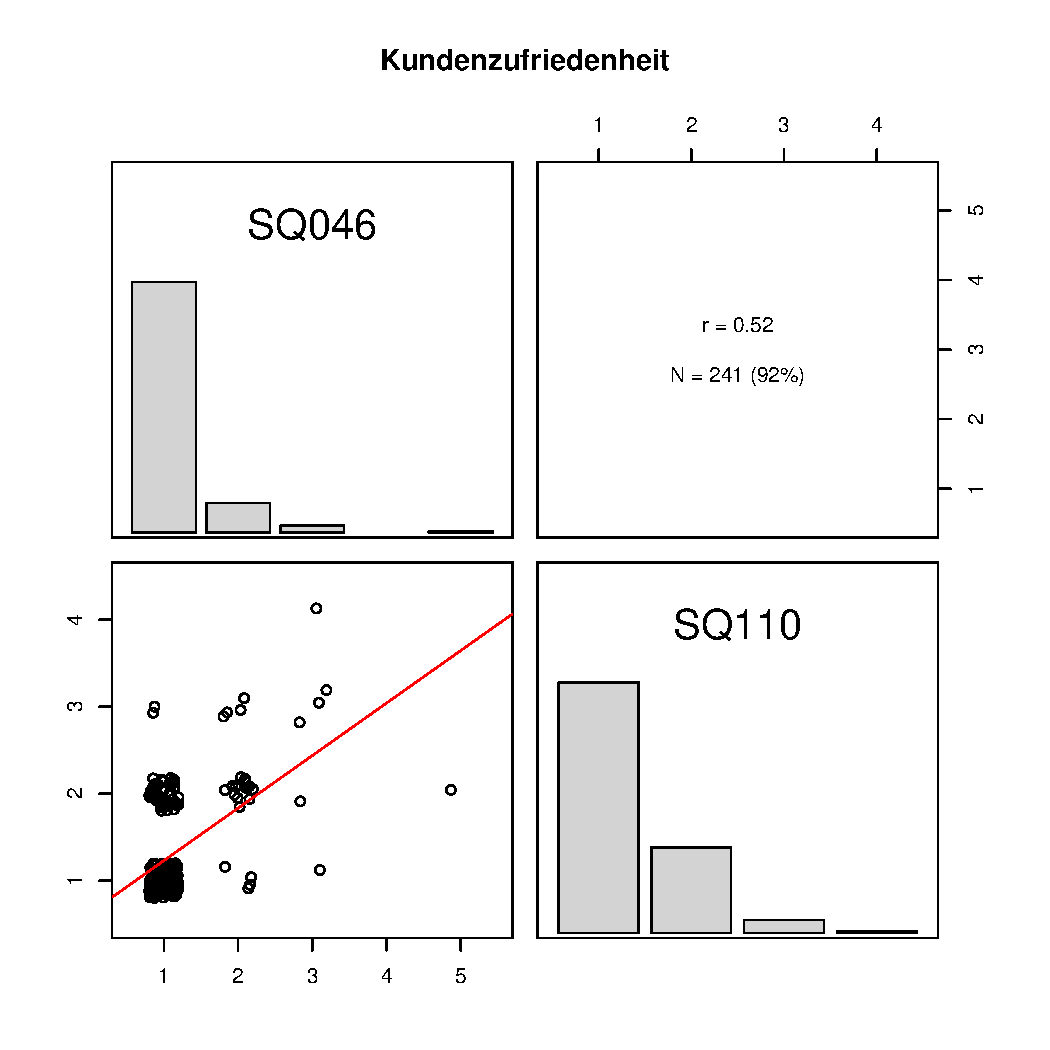
\includegraphics[width=\maxwidth]{figure/semPLS1} 
\begin{kframe}\begin{alltt}
\hlcom{#calculate model}
\hlstd{PB_model} \hlkwb{<-} \hlkwd{sempls}\hlstd{(}\hlkwc{model} \hlstd{= model,}\hlkwc{data} \hlstd{= CBdata)}
\end{alltt}
\begin{verbatim}
## Data rows: 4, 6, 15, 20, 21, 29, 32, 33, 34, 36, 37, 39, 43, 55, 58, 61, 72, 75, 76, 77, 80, 85, 90, 92, 95, 96, 97, 98, 100, 101, 102, 116, 128, 139, 144, 145, 153, 162, 163, 175, 176, 180, 184, 185, 186, 191, 192, 193, 197, 200, 206, 211, 218, 219, 224, 226, 227, 233, 235, 237, 240, 242, 245, 253, 258, 261 
## are not taken into acount, due to missings in the manifest variables.
##  Total number of complete cases: 195 
## Converged after 8 iterations.
## Tolerance: 1e-07
## Scheme: centroid
\end{verbatim}
\begin{alltt}
\hlcom{#show model}
\hlstd{PB_model}
\end{alltt}
\begin{verbatim}
##                                           Path Estimate
## lam_1_1                   Performance -> SQ079     0.93
## lam_1_2                   Performance -> SQ080     0.93
## lam_2_1                Preis_Leistung -> SQ009     0.84
## lam_2_2                Preis_Leistung -> SQ076     0.88
## lam_2_3                Preis_Leistung -> SQ092     0.76
## lam_2_4                Preis_Leistung -> SQ096    -0.48
## lam_2_5                Preis_Leistung -> SQ101     0.59
## lam_3_1           Kundenzufriedenheit -> SQ046     0.80
## lam_3_2           Kundenzufriedenheit -> SQ110     0.94
## beta_1_3    Performance -> Kundenzufriedenheit     0.42
## beta_2_3 Preis_Leistung -> Kundenzufriedenheit     0.34
\end{verbatim}
\begin{alltt}
\hlcom{#show all information in the object}
\hlkwd{summary}\hlstd{(PB_model)}
\end{alltt}
\begin{verbatim}
##                   Length Class      Mode     
## coefficients         2   data.frame list     
## path_coefficients    9   -none-     numeric  
## outer_loadings      27   -none-     numeric  
## cross_loadings      27   -none-     numeric  
## total_effects        9   -none-     numeric  
## inner_weights        9   -none-     numeric  
## outer_weights       27   -none-     numeric  
## blocks               0   -none-     NULL     
## factor_scores      585   -none-     numeric  
## data              1755   -none-     numeric  
## scaled               1   -none-     logical  
## model                8   plsm       list     
## weighting_scheme     1   -none-     character
## weights_evolution    4   data.frame list     
## sum1                 1   -none-     logical  
## pairwise             1   -none-     logical  
## method               1   -none-     character
## iterations           1   -none-     numeric  
## convCrit             1   -none-     character
## verbose              1   -none-     logical  
## tolerance            1   -none-     numeric  
## maxit                1   -none-     numeric  
## N                    1   -none-     numeric  
## incomplete          66   -none-     numeric  
## Hanafi              27   -none-     numeric
\end{verbatim}
\begin{alltt}
\hlcom{#to access parts of the object the $ operator is used f.e.}
\hlstd{PB_model}\hlopt{$}\hlstd{iterations}
\end{alltt}
\begin{verbatim}
## [1] 8
\end{verbatim}
\begin{alltt}
\hlcom{#load the Rgraphviz Package}
\hlkwd{library}\hlstd{(Rgraphviz)}

\hlcom{#visualize model with dot }
\hlcom{#graphviz required}
\hlkwd{pathDiagram}\hlstd{(PB_model,} \hlkwc{file} \hlstd{=} \hlstr{"PB-structure"}\hlstd{,} \hlkwc{edge.labels} \hlstd{=} \hlstr{"both"}\hlstd{,}
           \hlkwc{output.type} \hlstd{=} \hlstr{"graphics"}\hlstd{,} \hlkwc{digits} \hlstd{=} \hlnum{2}\hlstd{)}
\end{alltt}
\begin{verbatim}
## Running  dot -Tpdf -o PB-structure.pdf  PB-structure.dot
\end{verbatim}
\begin{alltt}
\hlstd{PBdot} \hlkwb{<-} \hlstr{"/home/jannic/PB-structure.dot"}
\hlstd{PBcom} \hlkwb{<-} \hlkwd{agread}\hlstd{(PBdot,} \hlkwc{layoutType}\hlstd{=}\hlstr{"dot"}\hlstd{)}
\hlkwd{plot}\hlstd{(PBcom,} \hlkwc{main}\hlstd{=}\hlstr{"Path model"}\hlstd{)}
\end{alltt}
\end{kframe}
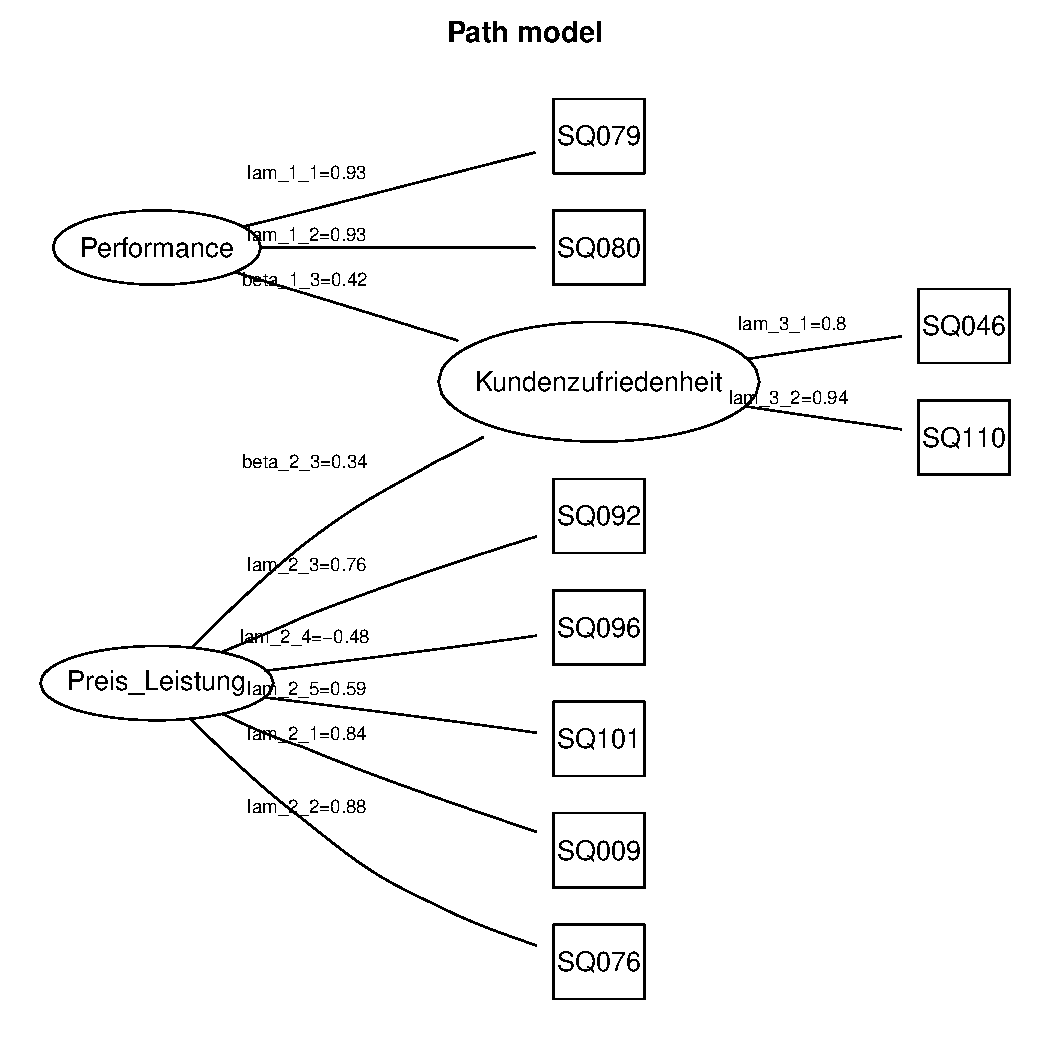
\includegraphics[width=\maxwidth]{figure/semPLS2} 

\end{knitrout}
Beschreibung zum Code:\\
Zunächst wird das Paket wieder in die aktuelle R-Session geladen und anschließend analog zu Kapitel 3.2.1 der Datensatz geladen. Für die Spezifizierung des Messmodells werden die Latenten Variablen, sowie die Indikatoren jeweils in einen Vektor geschrieben. Als nächster Schritt wird eine Matrix aus diesen gebildet und die Spaltennamen auf "source" und "target" gesetzt, um direkt ablesen zu können ob die Variablen reflektiv oder formativ gemessen werden. Das Strukturmodell wird analog zum Vorgehen beim Messmodell gebildet. Nachfolgend werden die einzelnen Teile mit der Funktion plsm() in ein Objekt geschrieben. Als Parameter werden der Datensatz, Messmodell und das Strukturmodell übergeben. Mit der Funktion mvpairs() können die Indikatoren der jeweiligen Latenten Variablen als Histogramm, Streudiagramm mit Regressiongeraden und die Pearson Korrelation mit der beachteten Fallzahl N dargestellt werden. Mit Hilfe des vorher erstellten Modell Objekt kann nun die Hauptfunktion sempls() des Pakets ausgeführt werden, welche zur Berechnung dient. Als Parameter erhält sie das Modell und den Datensatz. Das Weighting Scheme ist standardmäßig auf centroid gestellt falls es nicht als Parameter mitgegeben wird. Um die Ergebnisse aus SmartPLS und R besser vergleichen zu können empfiehlt es sich hier in beiden Programmen das gleiche Schema zu verwenden. Allerdings sind viele Autoren der Meinung, dass dies in der Berechnung keine großen Unterschiede erzeugt: "0.005 or less for structural path and 0.05 or less for measurement path".\cite{noonan1982pls} Anschließend kann über das schlichte Ausführen des Objektnamen PB\_model ein erster Überblick über das Modell erfolgen. Für weitere Analysen eignet sich der summary() Befehl, welcher die Verschiedenen im Objekt enthaltenen Daten anzeigt, die über den \$ Operator angesteuert werden können. Die Visualisierung erfolgt etwas umständlich über das Rgraphviz Paket, das zunächst geladen wird. Mit der pathDiagram() Funktion wird nun das Diagramm in DOT Sprache erstellt. Neben dem Modell und einem Namen können noch zahlreiche weitere Parameter übergeben werden, wie z.B. die Nachkommastellen mit digits=2, hierzu ist wieder die Hilfe Funktion help(pathDiagram) nützlich um die gewünschten Parameter einzustellen. Hier ist vor allem der Parameter full=FALSE zu erwähnen, da so nur das Strukturmodell visualisiert werden kann. Um die .dot Datei wieder in R darzustellen wird der Dateipfad in eine Variable gespeichert und dieser in die agread() Funktion als Parameter übergeben. Der layoutType wird auf "dot" gesetzt und anschließend kann die Graphik mit dem plot() Befehl angezeigt werden.\\
Zunächst scheint es als wäre die Modellspezifikation in R wesentlich aufwendiger als die Drag \& Drop Logik in SmartPLS. Allerdings können die Modelle aus SmartPLS mit dem semPLS Paket eingelesen werden. Somit kann das Modell in SmartPLS spezifiziert werden und weitere Berechnungen in R erfolgen. Alternativ kann die Spezifizierung in interaktiven Spreadsheets erfolgen. Nehmen wir z.B. die Matrix des Strukturmodells und führen folgenden Code aus:
\begin{knitrout}
\definecolor{shadecolor}{rgb}{0.969, 0.969, 0.969}\color{fgcolor}\begin{kframe}
\begin{alltt}
\hlkwd{data.entry}\hlstd{(CB_inner_model)}
\end{alltt}
\end{kframe}
\end{knitrout}
Nun können die Beziehung einfach in einem interaktiven Spreadsheet bearbeitet werden.\\

\subsubsection{knitr}
\href{http://cran.r-project.org/web/packages/knitr/index.html}{Knitr} ist ein Paket von \href{http://yihui.name/knitr/}{Yihui Xie} zur Erstellung von dynamischen Berichten in R mit Hilfe von Latex oder wahlweise auch Markdown. Es ist eine Weiterentwicklung von Sweave.\cite{lmucs-papers:Leisch:2002} Der Vorteil davon ist, dass der R Code zum einen automatisch mit Syntaxhervorhebung gekennzeichnet wird und zum anderen dass die Ergebnisse nicht zwischengespeichert und manuell in ein anderes Dokument eingefügt werden müssen. Falls zum Beispiel eine Änderung in einem Plot vorgenommen werden muss, wie eine falsche Beschriftung einer X-Achse zu korrigieren, muss dies nur im R Code geändert werden und die Datei kompiliert werden statt den Plot neu speichern und einfügen zu müssen. Außerdem sind der Bericht und Code in einem Dokument, was ebenfalls sehr hilfreich ist.\\
Die folgenden Erläuterungen waren bei der Erstellung dieses Berichts hilfreich, stellen jedoch nur einen Bruchteil der Möglichkeiten dar, welche dieses Paket bietet. Für eine ausführlichere Darstellung wird das Buch "Dynamic Documents with R and knitr" empfohlen.\cite{xie2013dynamic}\\
Zunächst wird das Paket installiert:
\begin{knitrout}
\definecolor{shadecolor}{rgb}{0.969, 0.969, 0.969}\color{fgcolor}\begin{kframe}
\begin{alltt}
\hlkwd{install.packages}\hlstd{(}\hlstr{"knitr"}\hlstd{)}
\end{alltt}
\end{kframe}
\end{knitrout}
Anschließend muss noch in R unter Tools -> Global Options -> Sweave -> Weave Rnw files using: auf knitr gesetzt werden. Nun kann unter File -> New File -> R Sweave ein neues Projekt erstellt werden. In diesem kann dann LaTeX Code geschrieben werden und mit der folgenden Syntax auch R Code eingebettet werden. Ein R Code Block wird mit $<<>>=$ begonnen und mit $@$ geschlossen. In den Anfangstag $<<>>=$ können weitere Parameter übergeben, welche den Output beeinflussen. Ohne Parameter wird der R Code mit Syntaxhervorhebung dargestellt, ausgeführt und die Ergebnisse wie Console Output und Plots ebenfalls in die PDF geschrieben. Dies geschieht mit dem Button "Compile PDF". Als erster Parameter kann ein Label, also Name für den Codeblock übergeben werden, um diesen später zu referenzieren oder lediglich schneller zu finden. Mit dem Parameter eval=FALSE wird verhindert dass der R-Code ausgeführt wird. Dieser eignet sich zum Beispiel bei install.packages oder nicht funktionierendem Code, da der Output in diesem Fall für den Leser nicht von Relevanz ist. Der Parameter include=FALSE führt dagegen den Code aus, aber die Ergebnisse dieser Ausführung werden nicht in den Bericht geschrieben. Dies ist zum Beispiel für das Laden von Paketen von Vorteil. Mit message=FALSE und warning=FALSE können Nachrichten und Warnungen im Bericht unterdrückt werden.
Mit dem Parameter echo=FALSE wird der Code nicht in den Bericht geschrieben, aber trotzdem ausgeführt und die Ergebnisse in den Bericht geschrieben. Der Parameter results='asis' schreibt die rohen Ergebnisse aus R direkt in den Bericht. Ein Beispiel dazu wird nachfolgend mit xtable gezeigt.\\
\\
Ein weiteres nützliches Paket ist das xtable Paket, welches aus R Objekten LaTeX oder HTML Tabellen erzeugen kann.
\begin{knitrout}
\definecolor{shadecolor}{rgb}{0.969, 0.969, 0.969}\color{fgcolor}\begin{kframe}
\begin{alltt}
\hlkwd{install.packages}\hlstd{(}\hlstr{"xtable"}\hlstd{)}
\end{alltt}
\end{kframe}
\end{knitrout}

\begin{knitrout}
\definecolor{shadecolor}{rgb}{0.969, 0.969, 0.969}\color{fgcolor}\begin{kframe}
\begin{alltt}
\hlcom{#load xtable package}
\hlkwd{library}\hlstd{(xtable)}
\end{alltt}
\end{kframe}
\end{knitrout}

\begin{knitrout}
\definecolor{shadecolor}{rgb}{0.969, 0.969, 0.969}\color{fgcolor}\begin{kframe}
\begin{alltt}
\hlcom{#print LaTeX Code}
\hlkwd{print}\hlstd{(}\hlkwd{xtable}\hlstd{(}\hlkwd{summary}\hlstd{(CB_PLS)}\hlopt{$}\hlstd{correlations))}
\end{alltt}
\begin{verbatim}
## % latex table generated in R 3.0.2 by xtable 1.7-4 package
## % Fri Jan  2 16:36:09 2015
## \begin{table}[ht]
## \centering
## \begin{tabular}{rrrr}
##   \hline
##  & Preis\_Leistung & Performance & Kundenzufriedenheit \\ 
##   \hline
## Preis\_Leistung & 1.00 & 0.52 & 0.75 \\ 
##   Performance & 0.52 & 1.00 & 0.34 \\ 
##   Kundenzufriedenheit & 0.75 & 0.34 & 1.00 \\ 
##    \hline
## \end{tabular}
## \end{table}
\end{verbatim}
\end{kframe}
\end{knitrout}

\begin{kframe}
\begin{alltt}
\hlcom{#print table with results='asis'}
\hlkwd{print}\hlstd{(}\hlkwd{xtable}\hlstd{(}\hlkwd{summary}\hlstd{(CB_PLS)}\hlopt{$}\hlstd{correlations))}
\end{alltt}
\end{kframe}% latex table generated in R 3.0.2 by xtable 1.7-4 package
% Fri Jan  2 16:36:09 2015
\begin{table}[ht]
\centering
\begin{tabular}{rrrr}
  \hline
 & Preis\_Leistung & Performance & Kundenzufriedenheit \\ 
  \hline
Preis\_Leistung & 1.00 & 0.52 & 0.75 \\ 
  Performance & 0.52 & 1.00 & 0.34 \\ 
  Kundenzufriedenheit & 0.75 & 0.34 & 1.00 \\ 
   \hline
\end{tabular}
\end{table}

Der Parameter results='asis' wird verwendet, da die Funktion xtable direkten LaTeX Code liefert und dieser so wie er ist kompiliert werden soll um die Tabelle im Bericht darzustellen anstatt des LaTeX Code. In der finalen Version sollte ebenfalls echo=FALSE verwendet werden, um den Befehl print xtable zu unterdrücken, da dieser lediglich zur Erzeugung einer ansprechenderen Tabelle dient und dem Leser sogesehen keinen zusätzlichen Nutzen bringt.\\
\\
Mit \verb!\Sexpr{}! kann eine Variable dynamisch in einen Text geschrieben werden, sodass diese zunächst berechnet und anschließend die Variable durch den Wert ersetzt wird. Der folgende R Code wählt beispielsweise eine Zahl von 1-10 zufällig aus und schreibt diese in die Variable x.
\begin{knitrout}
\definecolor{shadecolor}{rgb}{0.969, 0.969, 0.969}\color{fgcolor}\begin{kframe}
\begin{alltt}
\hlstd{x} \hlkwb{<-} \hlkwd{sample}\hlstd{(}\hlnum{1}\hlopt{:}\hlnum{10}\hlstd{,} \hlnum{1}\hlstd{)}
\end{alltt}
\end{kframe}
\end{knitrout}
Die Variable kann nun mit \lstinline!2! im Text refernziert werden:\\
Die Variable x hat den Wert 2.\\

\subsection{SmartPLS Modell einlesen}

Alternativ kann wie bereits erwähnt ein Modell aus SmartPLS importiert werden. Dazu muss das XML Paket installiert werden, da die Modellinformationen in XML Code gespeichert sind und nur so in R geladen werden können.\\
Für Ubuntu wird hier eine andere Methode zur Installation benötigt. Dazu wird einfach in ein Terminal der Befehl:
\begin{knitrout}
\definecolor{shadecolor}{rgb}{0.969, 0.969, 0.969}\color{fgcolor}\begin{kframe}
\begin{alltt}
\hlcom{#!ACHTUNG KEIN R-CODE!}
sudo apt-get install r-cran-xml
\end{alltt}
\end{kframe}
\end{knitrout}
eingegeben.\\
Je nach Betriebssystem kann jedoch auch nach der schon vorgestellten Methode in R installiert werden.
\begin{knitrout}
\definecolor{shadecolor}{rgb}{0.969, 0.969, 0.969}\color{fgcolor}\begin{kframe}
\begin{alltt}
\hlkwd{install.packages}\hlstd{(}\hlstr{"XML"}\hlstd{)}
\end{alltt}
\end{kframe}
\end{knitrout}

\begin{knitrout}
\definecolor{shadecolor}{rgb}{0.969, 0.969, 0.969}\color{fgcolor}\begin{kframe}
\begin{alltt}
\hlkwd{library}\hlstd{(XML)}

\hlcom{#get both filepaths}
\hlstd{dataPath} \hlkwb{<-} \hlstr{"/home/jannic/Schreibtisch/PB/Data/Datensatz.csv"}
\hlstd{modelPath} \hlkwb{<-} \hlstr{"/home/jannic/Schreibtisch/PB/Data/Modell.splsm"}

\hlcom{#read dataset}
\hlstd{mvdata} \hlkwb{<-} \hlkwd{read.csv}\hlstd{(dataPath)}
\end{alltt}


{\ttfamily\noindent\color{warningcolor}{\#\# Warning: kann Datei '/home/jannic/Schreibtisch/PB/Data/Datensatz.csv' nicht öffnen: No such file or directory}}

{\ttfamily\noindent\bfseries\color{errorcolor}{\#\# Error: kann Verbindung nicht öffnen}}\begin{alltt}
\hlcom{#read SmartPLS model}
\hlstd{splsmodel} \hlkwb{<-} \hlkwd{read.splsm}\hlstd{(modelPath)}
\end{alltt}


{\ttfamily\noindent\bfseries\color{errorcolor}{\#\# Error: XML content does not seem to be XML: '/home/jannic/Schreibtisch/PB/Data/Modell.splsm'}}\begin{alltt}
\hlcom{#show the model}
\hlstd{splsmodel}
\end{alltt}


{\ttfamily\noindent\bfseries\color{errorcolor}{\#\# Error: Objekt 'splsmodel' nicht gefunden}}\end{kframe}
\end{knitrout}

Zunächst wird das XML Paket in die R Session geladen und die zwei Dateipfade zu den in SmartPLS verwendeten Modell und Datensatz initialisiert. Dann wird der Datensatz wie bisher mit read.csv() eingelesen und anschließend das Modell mit der Funktion read.splsm() geladen. Nun kann das Modell angezeigt werden.\\
Hier sind jedoch zwei wesentliche Vorschriften zu beachten:
\begin{enumerate}
    \item Das SmartPLS Modell muss als splsm Datei gespeichert werden (nicht splsp!)
    \item Die csv Datei muss die selben Spaltennamen haben
\end{enumerate}
Der zweite Fall ist zu beachten, da die Benennung der Spalten mit eckigen Klammern: \\
F001[SQ001]\\
beim einlesen der csv Datei in R in:\\
F001..SQ001..\\
geändert werden. Daher empfiehlt es sich entweder schon in SmartPLS die csv Datei mit den Spaltennamen
SQ001 zu benutzen (2014\_08\_30-CB\_Alle\_R.csv) oder die Spaltennamen in R nach dem einlesen wieder in F001[SQ001] zu ändern, was jedoch wesentlich aufwendiger ist.\\
Anschließend können, wie bereits im vorherigen Kapitel beschrieben, die Berechnungen wie gewohnt durchgeführt werden.\\
\\


\subsection{Validation}
Die folgenden Ausführungen zur Validation stammen inhaltlich aus den Büchern PLS-Pfadmodellierung (S.71-87)\cite{bliemel2005handbuch}, A Primer on PLS-SEM (S.95-205)\cite{hair2013primer} und Strukturgleichungsmodellierung (S.325-337).\cite{weiber2010strukturgleichungsmodellierung} Letzteres wird jedoch nicht empfohlen, da dort die Validation reflektiver Messmodelle im PLS Ansatz gleich dem Kovarianzbasierten Ansatz gesetzt wird und Literaturangaben fehlen.
\subsubsection{reflektives Messmodell}
Die Validationsmethoden des Messmodells beziehen sich ausschließlich auf den reflektiven Ansatz, da die vorgestellten Modelle alle reflektiv spezifiziert wurden. Für eine formative Validation siehe "A primer on PLS-SEM"\cite{hair2013primer} Seite 118-166.\\

\paragraph{Inhaltsvaliditität} 

Grad, zu dem die Indikatoren dem inhaltlich-semantischen Bereich des Konstrukts angehören. Diese kann zum Beispiel mit Hilfe von Experten im Forschungsgebiet überprüft werden. Allerdings können auch die Intekorrelationen der Indikatoren eines Konstrukts auf Inhaltsvalidität hinweisen.\cite{hildebrandt1984kausalanalytische} Dazu eignet sich die explorative Faktorenanalyse.\cite{vinzi2003pls}\\
\begin{knitrout}
\definecolor{shadecolor}{rgb}{0.969, 0.969, 0.969}\color{fgcolor}\begin{kframe}
\begin{alltt}
\hlkwd{install.packages}\hlstd{(}\hlstr{"psych"}\hlstd{,}\hlstr{"GPArotation"}\hlstd{)}
\end{alltt}
\end{kframe}
\end{knitrout}
Zunächst werden die Pakete "psych" und "GPArotation" installiert.
\begin{knitrout}
\definecolor{shadecolor}{rgb}{0.969, 0.969, 0.969}\color{fgcolor}\begin{kframe}
\begin{alltt}
\hlkwd{library}\hlstd{(psych)}
\hlkwd{library}\hlstd{(GPArotation)}

\hlcom{#read in dataset (optional)}
\hlstd{CBdata} \hlkwb{<-} \hlkwd{read.csv}\hlstd{(}\hlstr{"/home/jannic/Schreibtisch/PB/Data/2014_08_30-CB_Alle_R.csv"}\hlstd{)}

\hlcom{#target indicators used in the model}
\hlstd{indicatorset} \hlkwb{<-} \hlstd{CBdata[}\hlkwd{c}\hlstd{(}\hlstr{"SQ009"}\hlstd{,}\hlstr{"SQ076"}\hlstd{,}\hlstr{"SQ092"}\hlstd{,}\hlstr{"SQ101"}\hlstd{,}\hlstr{"SQ096"}\hlstd{,}
                \hlstr{"SQ079"}\hlstd{,}\hlstr{"SQ080"}\hlstd{,}
                \hlstr{"SQ046"}\hlstd{,}\hlstr{"SQ110"}\hlstd{) ]}

\hlcom{#do parallel analysis}
\hlkwd{fa.parallel}\hlstd{(indicatorset,}\hlkwc{fa}\hlstd{=}\hlstr{"fa"}\hlstd{)}
\end{alltt}
\end{kframe}
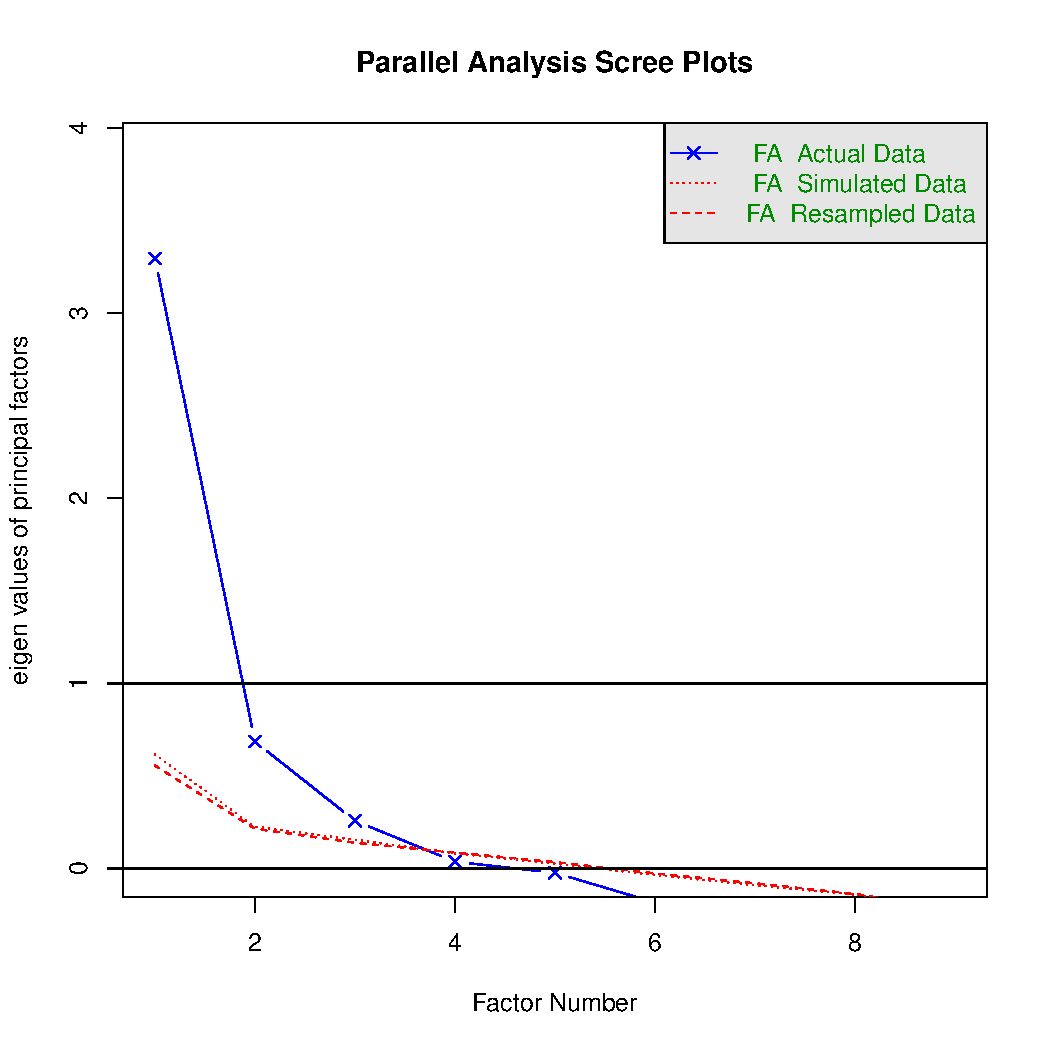
\includegraphics[width=\maxwidth]{figure/psych1} 
\begin{kframe}\begin{verbatim}
## Parallel analysis suggests that the number of factors =  3  and the number of components =  2
\end{verbatim}
\begin{alltt}
\hlcom{#do parallel analysis with polychoric correlations }
\hlkwd{fa.parallel.poly}\hlstd{(indicatorset,}\hlkwc{global}\hlstd{=}\hlnum{TRUE}\hlstd{,}\hlkwc{fa}\hlstd{=}\hlstr{"fa"}\hlstd{)}
\end{alltt}
\begin{verbatim}
## 
## 
## 
##  See the graphic output for a description of the results
\end{verbatim}
\end{kframe}
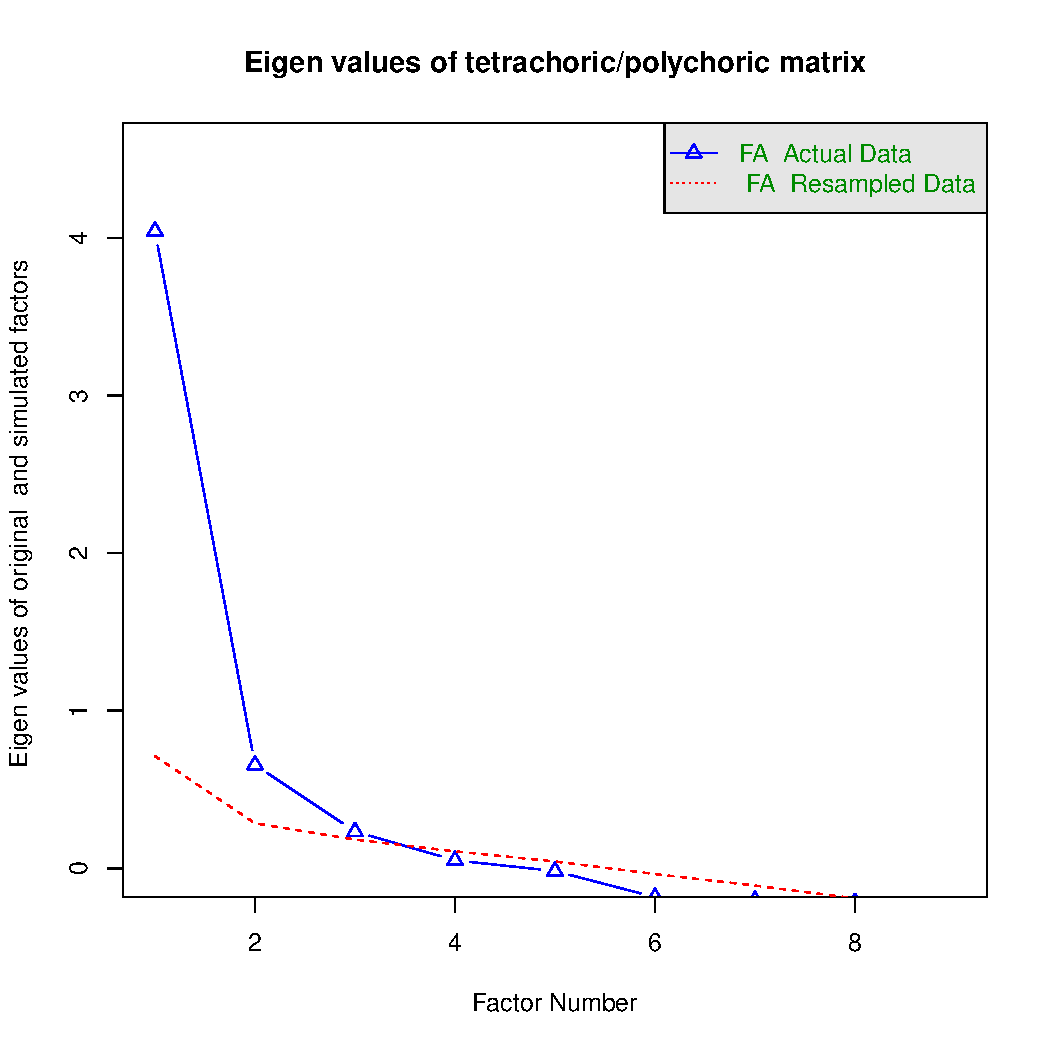
\includegraphics[width=\maxwidth]{figure/psych2} 
\begin{kframe}\begin{verbatim}
## Parallel analysis suggests that the number of factors =  3  and the number of components =  1
## Call: fa.parallel.poly(x = indicatorset, fa = "fa", global = TRUE)
## Parallel analysis suggests that the number of factors =  3  and the number of components =  1 
## 
##  Eigen Values of 
##   Original factors Simulated data Original components simulated data
## 1             4.04           0.68                4.55           1.49
## 2             0.66           0.31                1.22           1.26
## 3             0.23           0.19                0.85           1.14
\end{verbatim}
\begin{alltt}
\hlcom{#do factor analysis}
\hlstd{PB_fac} \hlkwb{<-} \hlkwd{fa}\hlstd{(indicatorset,} \hlkwc{nfactors}\hlstd{=}\hlnum{3}\hlstd{,} \hlkwc{rotate}\hlstd{=}\hlstr{"varimax"}\hlstd{)}

\hlcom{#do factor analysis with polychoric correlations}
\hlstd{PB_fac_poly} \hlkwb{<-} \hlkwd{fa.poly}\hlstd{(indicatorset,} \hlkwc{nfactors}\hlstd{=}\hlnum{3}\hlstd{,} \hlkwc{rotate}\hlstd{=}\hlstr{"varimax"}\hlstd{,}\hlkwc{global}\hlstd{=}\hlnum{TRUE}\hlstd{)}

\hlcom{#show results}
\hlkwd{print}\hlstd{(PB_fac}\hlopt{$}\hlstd{loadings,} \hlkwc{cut}\hlstd{=}\hlnum{0.3}\hlstd{)}
\end{alltt}
\begin{verbatim}
## 
## Loadings:
##       MR2    MR1    MR3   
## SQ009  0.784              
## SQ076  0.834              
## SQ092  0.465              
## SQ101  0.362         0.301
## SQ096 -0.483              
## SQ079         0.930       
## SQ080         0.668       
## SQ046                0.763
## SQ110         0.479  0.570
## 
##                  MR2   MR1   MR3
## SS loadings    2.074 1.713 1.252
## Proportion Var 0.230 0.190 0.139
## Cumulative Var 0.230 0.421 0.560
\end{verbatim}
\begin{alltt}
\hlkwd{print}\hlstd{(PB_fac_poly}\hlopt{$}\hlstd{fa}\hlopt{$}\hlstd{loadings,} \hlkwc{cut}\hlstd{=}\hlnum{0.3}\hlstd{)}
\end{alltt}
\begin{verbatim}
## 
## Loadings:
##       MR3    MR1    MR2   
## SQ009  0.765              
## SQ076  0.883              
## SQ092  0.513         0.332
## SQ101  0.444              
## SQ096 -0.506              
## SQ079         0.946       
## SQ080         0.658  0.360
## SQ046                0.942
## SQ110  0.399  0.458  0.586
## 
##                  MR3   MR1   MR2
## SS loadings    2.396 1.764 1.660
## Proportion Var 0.266 0.196 0.184
## Cumulative Var 0.266 0.462 0.647
\end{verbatim}
\begin{alltt}
\hlcom{#show initial Model}
\hlstd{PB_model}
\end{alltt}
\begin{verbatim}
##                                           Path Estimate
## lam_1_1                   Performance -> SQ079     0.93
## lam_1_2                   Performance -> SQ080     0.93
## lam_2_1                Preis_Leistung -> SQ009     0.84
## lam_2_2                Preis_Leistung -> SQ076     0.88
## lam_2_3                Preis_Leistung -> SQ092     0.76
## lam_2_4                Preis_Leistung -> SQ096    -0.48
## lam_2_5                Preis_Leistung -> SQ101     0.59
## lam_3_1           Kundenzufriedenheit -> SQ046     0.80
## lam_3_2           Kundenzufriedenheit -> SQ110     0.94
## beta_1_3    Performance -> Kundenzufriedenheit     0.42
## beta_2_3 Preis_Leistung -> Kundenzufriedenheit     0.34
\end{verbatim}
\begin{alltt}
\hlcom{#show diagram}
\hlkwd{fa.diagram}\hlstd{(PB_fac,} \hlkwc{main} \hlstd{=}\hlstr{"Factor Analysis"}\hlstd{)}
\end{alltt}
\end{kframe}
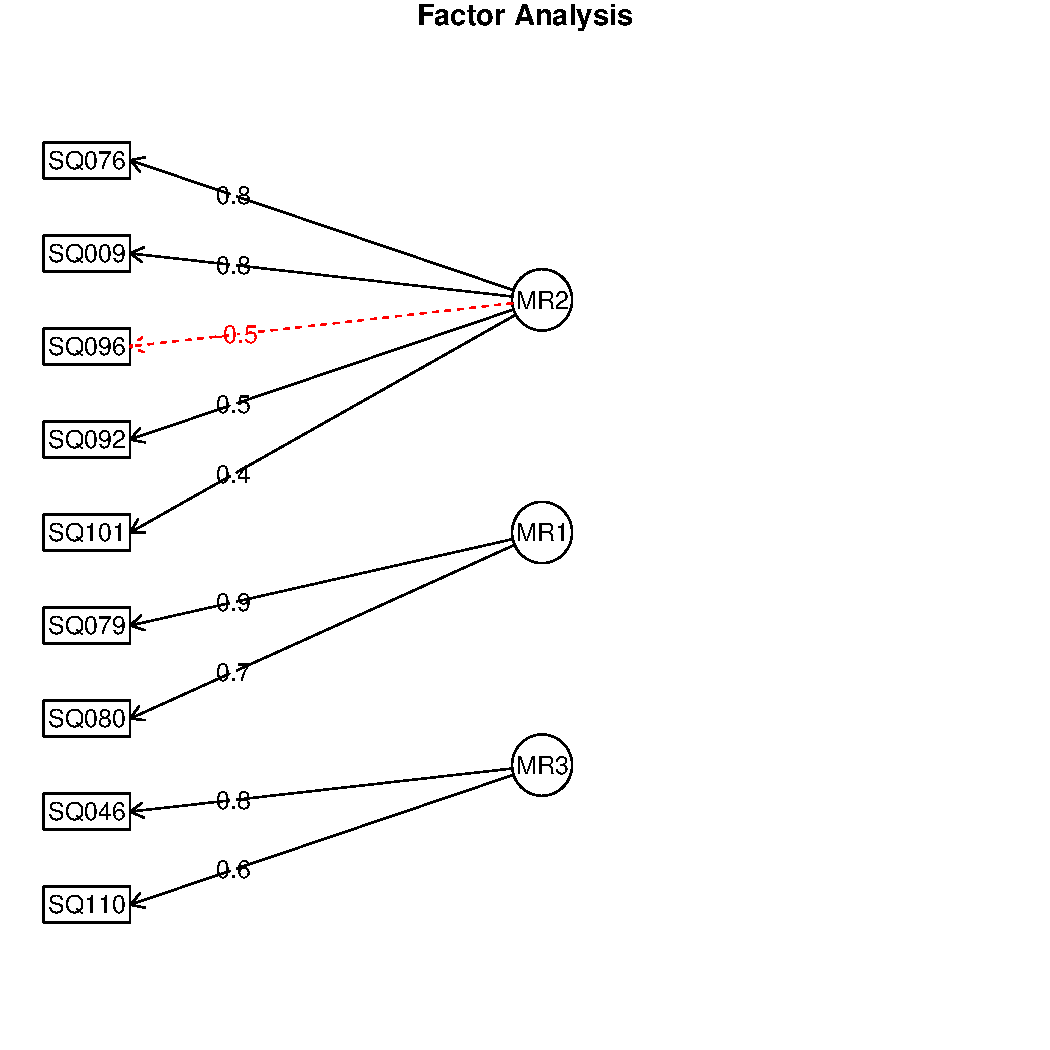
\includegraphics[width=\maxwidth]{figure/psych3} 
\begin{kframe}\begin{alltt}
\hlkwd{fa.diagram}\hlstd{(PB_fac_poly,} \hlkwc{main} \hlstd{=}\hlstr{"Factor Analysis polychoric"}\hlstd{)}
\end{alltt}
\end{kframe}
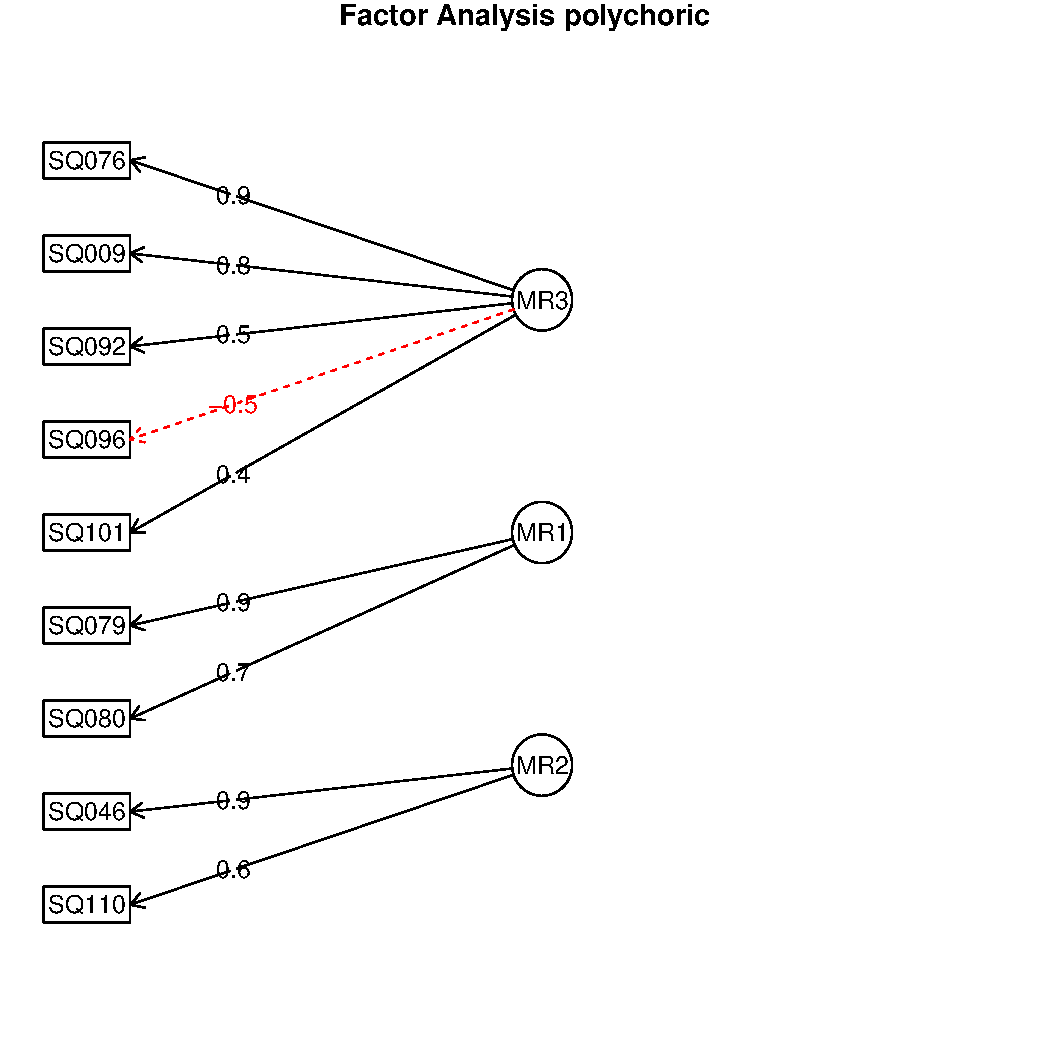
\includegraphics[width=\maxwidth]{figure/psych4} 

\end{knitrout}

Anschließend werden diese wie gewohnt in die R-Session geladen. Der Datensatz muss nicht noch einmal eingelesen werden, falls dies schon erfolgte. Hier wird dieser erneut eingelesen, da die explorative Faktorenanalyse auch vor der Modellspezifikation erfolgen kann und somit Konstrukte aus vorhandenen Daten gebildet werden statt diese persönlich manuell zu erstellen.\\
Zunächst muss der gewünschte Teildatensatz extrahiert werden. In diesem Fall wurden die Indikatoren bereits gewählt und daher werden diese auch als Teildatensatz für die Faktorenanalyse in der Variable "indicatorset" gespeichert. Alternativ könnten auch noch andere Indikatoren hinzugefügt werden von denen vermutet wird dass Sie zu einem spezifizierten Konstrukt passen. Um die Anzahl der Faktoren zu bestimmten, wird zunächst eine parallel Analyse nach Horn\cite{horn1965rationale} durchgeführt. Alternativ könnte auch in Scree-Test oder das Kaiser-Guttman-Kriterium herangezogen werden, allerdings herrscht in der Literatur Konsens darüber dass die parallel Analyse diesen überlegen ist.\cite{dinno2009exploring} Die nachfolgenden Berechnungen und Erklärungen sollen lediglich der Illustration dienen, da die Autoren der Meinung sind dass sich vorher mit der Methodik, den Annahmen und der Interpretation der Ergebnisse intensiver beschäftigt werden sollte, statt blind Funktionen auszuführen dessen Funktionsweise noch nicht gänzlich recherchiert wurde. Eine gute Einstiegsliteratur dazu ist beispielsweise Hayton's Tutorial zur parallel Analyse\cite{hayton2004factor} und das Kapitel zur explorativen Faktorenanalyse im Buch Multivariate Data Analysis von Hair et al.\cite{hair2006multivariate}\\
Die parallel Analyse wird mit der Funktion fa.parallel() aufgerufen und erhält als Parameter den Teil-Datensatz indicatorset, sowie fa="fa", das lediglich dazu dient die Hauptkomponentenanalyse nicht im Plot zu zeigen, da sie in diesem Fall nicht von Interesse ist. Zu beachten ist hier dass mehr Beobachtungen als Variablen in diesem Datensatz enthalten sein müssen. Dies ist in dem genannten Fall mit 261 Beobachtungen und 9 Variablen gewährleistet. Laut des Outputs in der Console werden 3 Faktoren vorgeschlagen. (Die Anzahl der Komponenten kann ignoriert werden, da eine Faktorenanalyse das Ziel ist und keine Hauptkomponentenanalyse). Dies ist ebenfalls im dazugehörigen Scree Plot zu sehen: Auf der X-Achse ist die Anzahl der Faktoren und auf der Y-Achse die Eigenwerte der Faktorenanalyse dargestellt. Die blaue durchgezogene Linie, unterbrochen durch Dreiecke stellt die Eigenwerte der Faktoren dar. Solange die Dreiecke oberhalb der gestrichelten roten Linie der Faktorenanalyse liegen, können diese Faktoren extrahiert werden. Die gestrichelte rote Linie stellt dabei die durchschnittlichen Eigenwerte von zufälligen, unkorrelierten, simulierten Daten dar.\\
Alternativ kann die parallel Analyse auch mit der polychorischen Korrelation statt des Bravais-Pearson Korrelationskoeffizienten berechnet werden, welche sich speziell für Likert-Skalen eignet.\cite{joreskog1986prelis} Dies geschieht in R mit der Funktion fa.parallel.poly(), welche die gleichen Parameter erhält, sowie eine zusätlichen global Parameter der auf TRUE gesetzt wird. Dieser soll dazu dienen zu signalisieren dass alle Variablen die gleiche Anzahl an Antwort Alternativen besitzen (In diesem Fall 1-5, sowie NA für fehlende Werte). Allerdings wird dieser laut Consolen Output wieder auf false gesetzt, da im Datensatz indicatorset Variablen enthalten sind dessen Beobachtungen nicht die volle Skala von 1-5 aufweisen, obwohl diese möglich wären. Für dieses Problem wurde noch keine Lösung erarbeitet und daher sollten die Ergebnisse dieser Berechnung kritisch angesehen werden. Der Consolen Output rät wieder zu einer Anzahl von 3 Faktoren, was ebenfalls wieder im Scree-Plot zu sehen ist. Da beide Verfahren die Faktorenanzahl von 3 liefern und im Vorhinein ebenfalls von 3 Faktoren (Preis\_Leistung, Performance, Kundenzufriedenheit) ausgegangen wurde, soll nun also die Faktorenanalyse mit 3 Faktoren angewendet werden.\\
Dazu wird die Methode fa(), mit dem Datensatz indicatorset, nfactors = 3 und rotation="varimax" als Parametern, aufgerufen. Nfactors gibt dabei die zuvor ermittelte Faktoren Anzahl von 3 und rotation die Rotationsmethode an. Diese wurde auf varimax gesetzt, da dies unterstellt dass die extrahierten Faktoren unabhängig voneinander sind. Da die Faktoren später nichts anderes als die Konstrukte, also latenten Variablen sind und diese sich inhaltlich unterscheiden sollten (siehe Diskriminanzvalidität) erscheint diese Rotationsmethode zweckmäßig. Die Wahl der Rotationsmethode besitzt eine gewisse Robustheit\cite{zwick1986comparison}, allerdings sollte bei der Anwendung die gewählte Methode Argumentativ gestützt werden oder die Ergebnisse unterschiedlicher Methoden verglichen werden. Für eine ausführliche Erläuterung der Rotationsmethoden siehe beispielweise Mulaik.\cite{mulaik1972foundations} Ebenfalls muss die Methode zur Faktorextrahierung ausgewählt werden. Dies geschieht mit dem Parameter fm, welcher als Standard auf fm="minres" gesetzt ist, für das minimales Residuum Verfahren. Auch hier sollte vorher recherchiert werden inwieweit sich diese unterscheiden und welche unter den gegebenen Daten am sinnvollsten erscheint oder auch verschiedene Ergebnisse verglichen werden. (siehe dazu auch Hayton S.193ff.\cite{hayton2004factor} ) Anschließend wird analog zur parallel Analyse die Faktorenanalyse mittels der fa.poly() Funktion mit polychorischen Korrelationen berechnet. Nun werden die Ergebnisse mit Hilfe der print() Funktion, welche als zusätlichen Parameter noch cut = 0.3 bekommt, in die Console geschrieben. Dieser Parameter dient lediglich der Übersichtlichkeit, er unterdrückt Werte die kleiner als 0.3 sind damit die Matrix der Ladungen besser leslich wird. Als Spalten werden nun die Faktoren MR1, MR2 und MR3 gelistet und als Zeilen die jeweiligen Indikatoren. Nun können die Konstrukte gebildet oder in diesem Fall überprüft werden. Dazu wird noch einmal PB\_model aufgerufen um die ursprünglichen Zuordnungen anzuzeigen.\\
Der Faktor ML2 weißt hohe Ladungen bei den Indikatoren SQ009, SQ076, SQ092, SQ101 und SQ096 auf. Dieser kann also als das Konstrukt Preis\_Leistung identifiziert werden. Generell sollten die Indikatoren die höchste Ladung bei dem Faktor aufzeigen, dem sie auch vorher in Form eines Konstrukts zugeordnet worden sind. Falls vorher noch keine Konstrukte gebildet wurden, werden die Fragen nach einem gemeinsamen inhaltlichen Kern abgesucht und anschließend ein dazu passender Name ausgedacht. Auf Faktor ML1 laden die Indikatoren SQ079 und SQ080 am höchsten, dies scheint also die latente Variable Performance zu sein. Abschließend laden SQ046 und SQ110 am höchsten auf ML3, welcher die Kundenzufriedenheit wiederspiegelt. Im Idealfall entsteht eine "Treppe" und die Indikatoren laden nur stark auf einen Faktor. Dies ist im gegeben Fall mit SQ101 und SQ110 nicht der Fall, da diese noch auf einen jeweils anderen Faktor laden. Das könnte nun durch eine Reihe von Umstrukturierungen versucht werden zu erreichen, allerdings stellt es auch den optimalen Fall dar und je nach Daten ist dieser auch schlichtweg nicht zu erreichen. Daher soll hier darauf verzichtet werden. Wird nun die Matrix der Ladungen der polychorischen Berechnungen betrachtet, können zwar unterschiedliche Werte festgestellt werden, allerdings laden die Indikatoren ebenfalls am höchsten auf das vorher spezifizierte Konstrukt. Zu beachten sind die unterschiedlichen Bezeichnungen der Faktoren. MR3 ist nun die latente Variable Preis\_Leistung, MR1 die Performance und MR2 die Kundenzufriedenheit. Da die Namen der Variablen vom Autor zugeordnet werden und dabei lediglich auf die Ladungen der Indikatoren geachtet wird, haben die veränderten Namen der Faktoren keinen Einfluss auf das Ergebnis.\\
Mit der fa.diagram() Funktion können die Ergebnisse auch in einem leicht verständlichen Diagramm dargestellt werden. Dieses sieht nun wie das mit dem semPLS Paket spezifizierte äußere Modell aus. Die Faktoren werden analog zu den Konstrukten im Strukturgleichungsmodell als Kreise dargestellt und die Indikatoren als Rechtecke. Die Ladungen stehen an den Pfeilen, welche Richtung der Indikatoren verlaufen, also reflektiv definiert sind. Hier ist ebenfalls zu sehen, dass sich die Berechnungen auf Basis von Pearson und polychorischen Korrelationen zwar in der Höhe einiger Ladungen unterscheiden, letztendlich jedoch zum gleichen Ergebnis kommen. Allerdings ist dies nicht immer der Fall und deshalb sollte überlegt werden welche Methode die geeignetere für einen gegebenen Datensatz darstellt. Im vorliegenden Fall sind die Autoren der Meinung, dass mit polychorischen Korrelationen gerechnet werden sollte, da die Daten mit Hilfe von Likert Skalen erhoben wurden.

\paragraph{Indikatorreliabilität} 

Die sogenannten äußeren Ladungen (outer loadings) wurden bereits mit der Funktion sempls() berechnet und können auch im Plot des Modells (lam\_x\_y = outer loadings) abgelesen werden. Hierbei handelt es sich um die Beziehungen zwischen Indikatoren und latenten Variablen, also des Messmodells. Äußere Gewichte (outer weights) wurden nicht berechnet, da das Modell rein reflektiv gemessen wurde. Bei einer formativen Messung und daraus resultierenden äußeren Gewichten gelten die nachfolgenden Erläuterungen zu äußeren Ladungen nicht. Die äußeren Ladungen geben von -1 bis 1 den Anteil der Varianz eines Indikators an, welcher durch seine latente Variable erklärt wird. Wird eine latente Variable nur mit einem einzigen Indikator gemessen ist die Ladung also logischerweise genau 1. Wird diese mit mehreren Indikatoren gemessen, sollten die Ladungen in der Regel über 0.7 sein.\cite{carmines1979reliability} Ladungen unter 0.4 sollten generell entfernt werden.\cite{hulland1999use} Für Ladungen von 0.4 bis 0.7 wird empfohlen die Auswirkungen des Löschens im Blick zu behalten und diese gegebenfalls nicht zu löschen, falls sich z.B. die Konstruktreliabilität nicht verbessert. Die Berechnung der Konstruktreliabilität wird im nächsten Abschnitt erläutert. Zunächst werden die Ladungen angezeigt:
\begin{knitrout}
\definecolor{shadecolor}{rgb}{0.969, 0.969, 0.969}\color{fgcolor}\begin{kframe}
\begin{alltt}
\hlstd{PB_model}\hlopt{$}\hlstd{outer_loadings}
\end{alltt}
\begin{verbatim}
##       Performance Preis_Leistung Kundenzufriedenheit
## SQ079      0.9288         0.0000              0.0000
## SQ080      0.9339         0.0000              0.0000
## SQ009      0.0000         0.8429              0.0000
## SQ076      0.0000         0.8800              0.0000
## SQ092      0.0000         0.7562              0.0000
## SQ096      0.0000        -0.4799              0.0000
## SQ101      0.0000         0.5937              0.0000
## SQ046      0.0000         0.0000              0.7989
## SQ110      0.0000         0.0000              0.9416
\end{verbatim}
\end{kframe}
\end{knitrout}
Beim Konstrukt Preis\_Leistung sind die Ladungen der Indikatoren SQ096 und SQ101 unter den gewünschten 0.7, jedoch noch über dem Minimum von 0.4. Hier muss also abgewogen werden ob diese gelöscht werden sollten. Da sich die Konstruktreliabilität von 0.74 auf 0.89 verbessert werden diese entfernt und es entsteht das folgende Modell: 
\begin{knitrout}
\definecolor{shadecolor}{rgb}{0.969, 0.969, 0.969}\color{fgcolor}\begin{kframe}
\begin{alltt}
\hlcom{#specify new model}
\hlstd{new_PB_model} \hlkwb{<-} \hlkwd{sempls}\hlstd{(}\hlkwc{model} \hlstd{=} \hlkwd{plsm}\hlstd{(}\hlkwc{data} \hlstd{= CBdata,}
                \hlkwc{strucmod} \hlstd{=} \hlkwd{cbind}\hlstd{(}\hlkwd{c}\hlstd{(}\hlstr{"Preis_Leistung"}\hlstd{,}\hlstr{"Performance"}\hlstd{),}
                                 \hlkwd{c}\hlstd{(}\hlkwd{rep}\hlstd{(}\hlstr{"Kundenzufriedenheit"}\hlstd{,}\hlnum{2}\hlstd{))),}
                \hlkwc{measuremod} \hlstd{=} \hlkwd{cbind}\hlstd{(}\hlkwd{c}\hlstd{(}\hlkwd{rep}\hlstd{(}\hlstr{"Preis_Leistung"}\hlstd{,}\hlnum{3}\hlstd{),}
                                     \hlkwd{rep}\hlstd{(}\hlstr{"Performance"}\hlstd{,}\hlnum{2}\hlstd{),}
                                     \hlkwd{rep}\hlstd{(}\hlstr{"Kundenzufriedenheit"}\hlstd{,}\hlnum{2}\hlstd{)),}
                                   \hlkwd{c}\hlstd{(}\hlstr{"SQ009"}\hlstd{,}\hlstr{"SQ076"}\hlstd{,}\hlstr{"SQ092"}\hlstd{,}\hlstr{"SQ079"}\hlstd{,}
                                     \hlstr{"SQ080"}\hlstd{,}\hlstr{"SQ046"}\hlstd{,}\hlstr{"SQ110"}\hlstd{)))}
                \hlstd{,}\hlkwc{data} \hlstd{= CBdata)}
\end{alltt}
\begin{verbatim}
## Data rows: 4, 6, 20, 29, 32, 33, 36, 37, 39, 43, 55, 61, 72, 76, 77, 80, 90, 92, 95, 96, 97, 100, 101, 102, 116, 139, 144, 145, 153, 162, 163, 175, 176, 184, 185, 186, 192, 193, 197, 218, 224, 227, 233, 235, 237, 240, 242, 245, 253, 258, 261 
## are not taken into acount, due to missings in the manifest variables.
##  Total number of complete cases: 210 
## Converged after 7 iterations.
## Tolerance: 1e-07
## Scheme: centroid
\end{verbatim}
\begin{alltt}
\hlcom{#show old model}
\hlstd{PB_model}
\end{alltt}
\begin{verbatim}
##                                           Path Estimate
## lam_1_1                   Performance -> SQ079     0.93
## lam_1_2                   Performance -> SQ080     0.93
## lam_2_1                Preis_Leistung -> SQ009     0.84
## lam_2_2                Preis_Leistung -> SQ076     0.88
## lam_2_3                Preis_Leistung -> SQ092     0.76
## lam_2_4                Preis_Leistung -> SQ096    -0.48
## lam_2_5                Preis_Leistung -> SQ101     0.59
## lam_3_1           Kundenzufriedenheit -> SQ046     0.80
## lam_3_2           Kundenzufriedenheit -> SQ110     0.94
## beta_1_3    Performance -> Kundenzufriedenheit     0.42
## beta_2_3 Preis_Leistung -> Kundenzufriedenheit     0.34
\end{verbatim}
\begin{alltt}
\hlcom{#show new model}
\hlstd{new_PB_model}
\end{alltt}
\begin{verbatim}
##                                           Path Estimate
## lam_1_1                   Performance -> SQ079     0.92
## lam_1_2                   Performance -> SQ080     0.92
## lam_2_1                Preis_Leistung -> SQ009     0.86
## lam_2_2                Preis_Leistung -> SQ076     0.90
## lam_2_3                Preis_Leistung -> SQ092     0.80
## lam_3_1           Kundenzufriedenheit -> SQ046     0.79
## lam_3_2           Kundenzufriedenheit -> SQ110     0.94
## beta_1_3    Performance -> Kundenzufriedenheit     0.43
## beta_2_3 Preis_Leistung -> Kundenzufriedenheit     0.29
\end{verbatim}
\end{kframe}
\end{knitrout}
Der Code wurde hier auf das nötigste reduziert, da dieser bereits im Kapitel semPLS ausführlicher dargestellt wurde. Auf die Konstruktreliabilität wird im nächsten Abschnitt eingegangen. Neben den verbesserten Ladungen und damit der Konstruktreliabilität durch das Löschen ist jedoch auch zu sehen, dass der Pfadkoeffizient von Preis\_Leistung zu Kundenzufriedenheit von 0.34 auf 0.29 gesunken ist. Hier müssen also die Vor- und Nachteile wie bereits erwähnt abgewogen werden. Im Idealfall lässt sich ein anderer Indikator finden, welcher beide Werte verbessert. Da das Modell jedoch nur zur Demonstration dient, wird dies an dieser Stelle jedoch unterlassen.

\paragraph{Konstruktreliabilität} 

Nun wird die "Interne Konsistenz" (composite reliability) berechnet. Diese gibt an wie gut ein Konstrukt durch seine Indikatoren repräsentiert wird. Dabei können Werte von 0 bis 1 entstehen. Die Formel dazu lautet nach Fornell \& Larcker:\cite{fornell1981structural}
\begin{equation}
\rho_{c} = \frac{(\sum_{i}^{}\lambda_{ij})^{2}}{(\sum_{i}^{}\lambda_{ij})^{2}+\sum_{i}^{}var(\epsilon_{ij})}
\end{equation}
mit:\\
\begin{tabular}{llll}
$\lambda_{i}$  &= Ladung der Indikatorvariable i\\
$\epsilon_{i}$ &= Messfehler der Indikatorvariable i\\
j  &= Laufindex über alle reflektiven Messmodelle\\
$var(\epsilon_{i})$ &= Varianz des Messfehlers\\
\end{tabular}
\\
Die korrespondierende Funktion heißt im semPLS Paket dgrho() und erhält als einzigen Parameter das Modell.
\begin{knitrout}
\definecolor{shadecolor}{rgb}{0.969, 0.969, 0.969}\color{fgcolor}\begin{kframe}
\begin{alltt}
\hlkwd{dgrho}\hlstd{(PB_model)}
\end{alltt}
\begin{verbatim}
##                     Dillon-Goldstein's rho reflective MVs
## Performance                           0.93              2
## Preis_Leistung                        0.74              5
## Kundenzufriedenheit                   0.86              2
\end{verbatim}
\begin{alltt}
\hlkwd{dgrho}\hlstd{(new_PB_model)}
\end{alltt}
\begin{verbatim}
##                     Dillon-Goldstein's rho reflective MVs
## Performance                           0.92              2
## Preis_Leistung                        0.89              3
## Kundenzufriedenheit                   0.86              2
\end{verbatim}
\end{kframe}
\end{knitrout}
Hier erkennt man die Steigerung des rho der latenten Variable Preis\_Leistung von 0.74 im alten Modell auf 0.89 im neuen Modell, welche durch das löschen der Indikatoren SQ096 und SQ101 erreicht wurde. Außerdem liegen alle rhos über den in der Literatur üblichen Empfehlungen von mindestens 0.6 bis 0.7.\cite{nunnally1978c,bagozzi1988evaluation} Allerdings muss bei zu hohen Werten (>0.95) untersucht werden ob die Indikatoren nicht eventuell einfach das gleiche messen.

\paragraph{Diskriminanzvalidität} 

Darunter wird die Unterschiedlichkeit der Messungen verschiedener Konstrukte mit einem Messinstrument verstanden. Vereinfacht bedeutet dies, dass ein Konstrukt einzigartig sein sollte und sich daher von anderen Kontrukten unterscheiden sollte. Gemessen werden kann dies unter anderem mit dem Fornell \& Larcker Kriterium\cite{fornell1981structural}, welches besagt dass die gemeinsame Varianz zwischen einer latenten Variablen und ihren Indikatoren größer sein soll als die gemeinsame Varianz mit anderen latenten Variablen. Hierzu wird zunächst die durchschnittlich erfasste Varianz nach der folgenden Formel berechnet:
\begin{equation}
DEV = \sum_{i}^{}\frac{\lambda_{i}^{2}}{\sum_{i}^{}\lambda_{i}^{2}+\sum_{i}^{}var(\epsilon_{i})}
\end{equation}
mit:\\
\begin{tabular}{lll}
$\lambda_{i}$  &= Ladung der Indikatorvariable i\\
$\epsilon_{i}$ &= Messfehler der Indikatorvariable i\\
$var(\epsilon_{i})$ &= Varianz des Messfehlers\\
\end{tabular}
Eine durchschnittlich erfasste Varianz von bspw. 0.5 bedeutet hier, dass das Konstrukt im Mittel 50\% der Varianz seiner Indikatoren erklärt. Dies stellt gleichzeitig den empfohlenen Mindestwert dar, weil sonst der überwiegende Teil der Varianz auf den Fehlerterm entfällt.\cite{homburg1996konzeptualisierung,rodgers2003developing}
Im semPLS Paket heißt die korrespondierende Funktion communality().
\begin{knitrout}
\definecolor{shadecolor}{rgb}{0.969, 0.969, 0.969}\color{fgcolor}\begin{kframe}
\begin{alltt}
\hlkwd{communality}\hlstd{(PB_model)}
\end{alltt}
\begin{verbatim}
##                     communality reflective MVs
## Performance                0.87              2
## Preis_Leistung             0.53              5
## Kundenzufriedenheit        0.76              2
## 
## 	Average communality: 0.66
\end{verbatim}
\begin{alltt}
\hlstd{PB_model}\hlopt{$}\hlstd{path_coefficients}\hlopt{^}\hlnum{2}
\end{alltt}
\begin{verbatim}
##                     Performance Preis_Leistung Kundenzufriedenheit
## Performance                   0              0              0.1750
## Preis_Leistung                0              0              0.1165
## Kundenzufriedenheit           0              0              0.0000
\end{verbatim}
\begin{alltt}
\hlkwd{communality}\hlstd{(new_PB_model)}
\end{alltt}
\begin{verbatim}
##                     communality reflective MVs
## Performance                0.85              2
## Preis_Leistung             0.73              3
## Kundenzufriedenheit        0.76              2
## 
## 	Average communality: 0.77
\end{verbatim}
\begin{alltt}
\hlstd{new_PB_model}\hlopt{$}\hlstd{path_coefficients}\hlopt{^}\hlnum{2}
\end{alltt}
\begin{verbatim}
##                     Performance Preis_Leistung Kundenzufriedenheit
## Performance                   0              0             0.18424
## Preis_Leistung                0              0             0.08654
## Kundenzufriedenheit           0              0             0.00000
\end{verbatim}
\end{kframe}
\end{knitrout}
Ist nun die jeweils ermittelte durchschnittlich erfasste Varianz eines Konstrukts höher als jede quadrierte Korrelation mit einem anderen Konstrukt, ist das Fornell \& Larcker Kriterium erfüllt. Dies ist im alten, sowie im neuen Modell gegeben. Beachte auch die gesteigerte DEV der Preis\_Leistung im neuen Modell, welche sich durch das Löschen der zwei Indikatoren ergibt.\\
\\
Eine weitere Methode die Diskriminanzvalidität zu überprüfen stellt das Analysieren der "cross loadings" dar.
\begin{knitrout}
\definecolor{shadecolor}{rgb}{0.969, 0.969, 0.969}\color{fgcolor}\begin{kframe}
\begin{alltt}
\hlstd{PB_model}\hlopt{$}\hlstd{cross_loadings}
\end{alltt}
\begin{verbatim}
##       Performance Preis_Leistung Kundenzufriedenheit
## SQ079      0.9288         0.4307              0.5226
## SQ080      0.9339         0.4056              0.5417
## SQ009      0.3375         0.8429              0.4125
## SQ076      0.4162         0.8800              0.4777
## SQ092      0.3809         0.7562              0.4040
## SQ096     -0.2130        -0.4799             -0.1204
## SQ101      0.2399         0.5937              0.3743
## SQ046      0.2852         0.3664              0.7989
## SQ110      0.6341         0.5297              0.9416
\end{verbatim}
\begin{alltt}
\hlstd{new_PB_model}\hlopt{$}\hlstd{cross_loadings}
\end{alltt}
\begin{verbatim}
##       Performance Preis_Leistung Kundenzufriedenheit
## SQ079      0.9227         0.4009              0.5190
## SQ080      0.9180         0.3933              0.5046
## SQ009      0.3036         0.8600              0.3790
## SQ076      0.4129         0.8974              0.4505
## SQ092      0.3807         0.7993              0.3920
## SQ046      0.2897         0.3117              0.7927
## SQ110      0.6071         0.4893              0.9424
\end{verbatim}
\end{kframe}
\end{knitrout}
Hier sollten die Ladungen der Indikatoren auf das im Modell entsprechend zugeordnete Konstrukt am höchsten sein und idealerweise, jedoch nicht notwendigerweise die Ladungen auf andere Konstrukte unter 0.7 betragen. Dies ist sowohl im Ausgangsmodell als auch im neuen Modell erfüllt.\\
\\
Damit sind alle Kriterien an das reflektive Messmodell erfüllt. Bei komplexen Modellen sind diese Kennzahlen nicht immer alle erfüllt, jedoch liefern sie wertvolle Maßzahlen an denen sich Ersteller des Modells bei der Spezifikation orientieren kann. Am Ende sollte der Ersteller sich allerdings nicht  ausschließlich auf diese Kennzahlen verlassen und jegliche Logik ausschalten, sondern diese auch kritisch hinterfragen, sowie das Gesamtmodell im Auge behalten. So könnte z.B. durch reine Beachtung der Kennzahlen ein Modell, welches diese perfekt erfüllt erstellt werden, jedoch am Ende die für den Ersteller eigentlich wichtigen latenten Variablen gar nicht oder nur schlecht erklärt.

\subsubection{Strukturmodell}

\paragraph{Pfadkoeffizienten}

Die Pfadkoeffizienten (path coefficients) wurden bereits mit der Funktion sempls() berechnet und können auch im Plot des Modells (beta\_x\_y = path coefficients) abgelesen werden. Hierbei handelt es sich um die direkten Beziehungen zwischen den latenten Variablen, also des Strukturmodells. Diese werden mit standardisierten Werten angezeigt, welche von -1 über 0 bis 1 reichen. Hier repräsentieren Werte nahe 1 einen starken positiven Zusammenhang, nahe 0 einen schwachen und nahe -1 einen stark negativen Zusammenhang. Interessant sind ebenfalls die "total effects", d.h. die Summe der direkten und indirekten Beziehungen. Da im vorgestellten Modell jedoch keine Konstrukte zwischen der endogenen Variable Kundenzufriedenheit und den exogenen Variablen Performance und Preis\_Leistung liegen, es also keine indirekten Beziehungen gibt, sind "total effects" und "path coefficients" äquivalent.
\begin{knitrout}
\definecolor{shadecolor}{rgb}{0.969, 0.969, 0.969}\color{fgcolor}\begin{kframe}
\begin{alltt}
\hlstd{PB_model}\hlopt{$}\hlstd{path_coefficients}
\end{alltt}
\begin{verbatim}
##                     Performance Preis_Leistung Kundenzufriedenheit
## Performance                   0              0              0.4183
## Preis_Leistung                0              0              0.3414
## Kundenzufriedenheit           0              0              0.0000
\end{verbatim}
\begin{alltt}
\hlstd{PB_model}\hlopt{$}\hlstd{total_effects}
\end{alltt}
\begin{verbatim}
##                     Performance Preis_Leistung Kundenzufriedenheit
## Performance                   0              0              0.4183
## Preis_Leistung                0              0              0.3414
## Kundenzufriedenheit           0              0              0.0000
\end{verbatim}
\begin{alltt}
\hlstd{new_PB_model}\hlopt{$}\hlstd{path_coefficients}
\end{alltt}
\begin{verbatim}
##                     Performance Preis_Leistung Kundenzufriedenheit
## Performance                   0              0              0.4292
## Preis_Leistung                0              0              0.2942
## Kundenzufriedenheit           0              0              0.0000
\end{verbatim}
\begin{alltt}
\hlstd{new_PB_model}\hlopt{$}\hlstd{total_effects}
\end{alltt}
\begin{verbatim}
##                     Performance Preis_Leistung Kundenzufriedenheit
## Performance                   0              0              0.4292
## Preis_Leistung                0              0              0.2942
## Kundenzufriedenheit           0              0              0.0000
\end{verbatim}
\end{kframe}
\end{knitrout}

\paragraph{Bootstrapping}

Die Zuverlässigkeit der Pfadkoeffizienten kann mittels der Bootstrapping Methode ermittelt werden. Hierbei werden eine bestimmte Anzahl und Größe an Teilmengen zufällig aus dem original Datensatz gezogen und jeweils mit diesen Teilmengen das Modell berechnet. Somit erhält man Intervalle mit durchschnitts, minimalen, maximalen Werten, sowie Standardfehler der jeweiligen Beziehung.

\begin{knitrout}
\definecolor{shadecolor}{rgb}{0.969, 0.969, 0.969}\color{fgcolor}\begin{kframe}
\begin{alltt}
\hlcom{#create seed with arbitrary number}
\hlkwd{set.seed}\hlstd{(}\hlnum{123}\hlstd{)}

\hlcom{#execute algorithm}
\hlstd{new_PB_model_boot} \hlkwb{<-} \hlkwd{bootsempls}\hlstd{(new_PB_model,} \hlkwc{nboot}\hlstd{=}\hlnum{200}\hlstd{,} \hlkwc{verbose}\hlstd{=}\hlnum{FALSE}\hlstd{)}

\hlcom{#show results}
\hlstd{new_PB_model_boot}
\end{alltt}
\begin{verbatim}
## Call: bootsempls(object = new_PB_model, nboot = 200, verbose = FALSE)
## 
##                                       Estimate     Bias Std.Error
## Performance -> SQ079                     0.923  0.00131   0.01311
## Performance -> SQ080                     0.918  0.00197   0.01724
## Preis_Leistung -> SQ009                  0.860  0.00012   0.02546
## Preis_Leistung -> SQ076                  0.897  0.00133   0.01508
## Preis_Leistung -> SQ092                  0.799 -0.00265   0.03463
## Kundenzufriedenheit -> SQ046             0.793 -0.00402   0.06372
## Kundenzufriedenheit -> SQ110             0.942  0.00206   0.00925
## Performance -> Kundenzufriedenheit       0.429  0.00832   0.07462
## Preis_Leistung -> Kundenzufriedenheit    0.294 -0.00181   0.07521
\end{verbatim}
\begin{alltt}
\hlcom{#give a summary}
\hlkwd{summary}\hlstd{(new_PB_model_boot,} \hlkwc{level}\hlstd{=}\hlnum{0.95}\hlstd{)}
\end{alltt}
\begin{verbatim}
## Call: bootsempls(object = new_PB_model, nboot = 200, verbose = FALSE)
## 
## Lower and upper limits are for the 95 percent perc confidence interval
## 
##          Estimate     Bias Std.Error Lower Upper
## lam_1_1     0.923  0.00131   0.01311 0.892 0.943
## lam_1_2     0.918  0.00197   0.01724 0.877 0.947
## lam_2_1     0.860  0.00012   0.02546 0.804 0.907
## lam_2_2     0.897  0.00133   0.01508 0.865 0.927
## lam_2_3     0.799 -0.00265   0.03463 0.719 0.859
## lam_3_1     0.793 -0.00402   0.06372 0.642 0.898
## lam_3_2     0.942  0.00206   0.00925 0.926 0.966
## beta_1_3    0.429  0.00832   0.07462 0.280 0.589
## beta_2_3    0.294 -0.00181   0.07521 0.120 0.417
\end{verbatim}
\begin{alltt}
\hlcom{#get coefficient names}
\hlstd{new_PB_model_boot}\hlopt{$}\hlstd{fitted_model}
\end{alltt}
\begin{verbatim}
##                                           Path Estimate
## lam_1_1                   Performance -> SQ079     0.92
## lam_1_2                   Performance -> SQ080     0.92
## lam_2_1                Preis_Leistung -> SQ009     0.86
## lam_2_2                Preis_Leistung -> SQ076     0.90
## lam_2_3                Preis_Leistung -> SQ092     0.80
## lam_3_1           Kundenzufriedenheit -> SQ046     0.79
## lam_3_2           Kundenzufriedenheit -> SQ110     0.94
## beta_1_3    Performance -> Kundenzufriedenheit     0.43
## beta_2_3 Preis_Leistung -> Kundenzufriedenheit     0.29
\end{verbatim}
\begin{alltt}
\hlcom{#plot bootstrap samples}
\hlkwd{parallelplot}\hlstd{(new_PB_model_boot,} \hlkwc{subset}\hlstd{=}\hlnum{1}\hlopt{:}\hlkwd{ncol}\hlstd{(new_PB_model_boot}\hlopt{$}\hlstd{t),} \hlkwc{reflinesAt}\hlstd{=}\hlkwd{c}\hlstd{(}\hlopt{-}\hlnum{1}\hlstd{,}\hlnum{0}\hlstd{,}\hlnum{1}\hlstd{))}
\end{alltt}
\end{kframe}
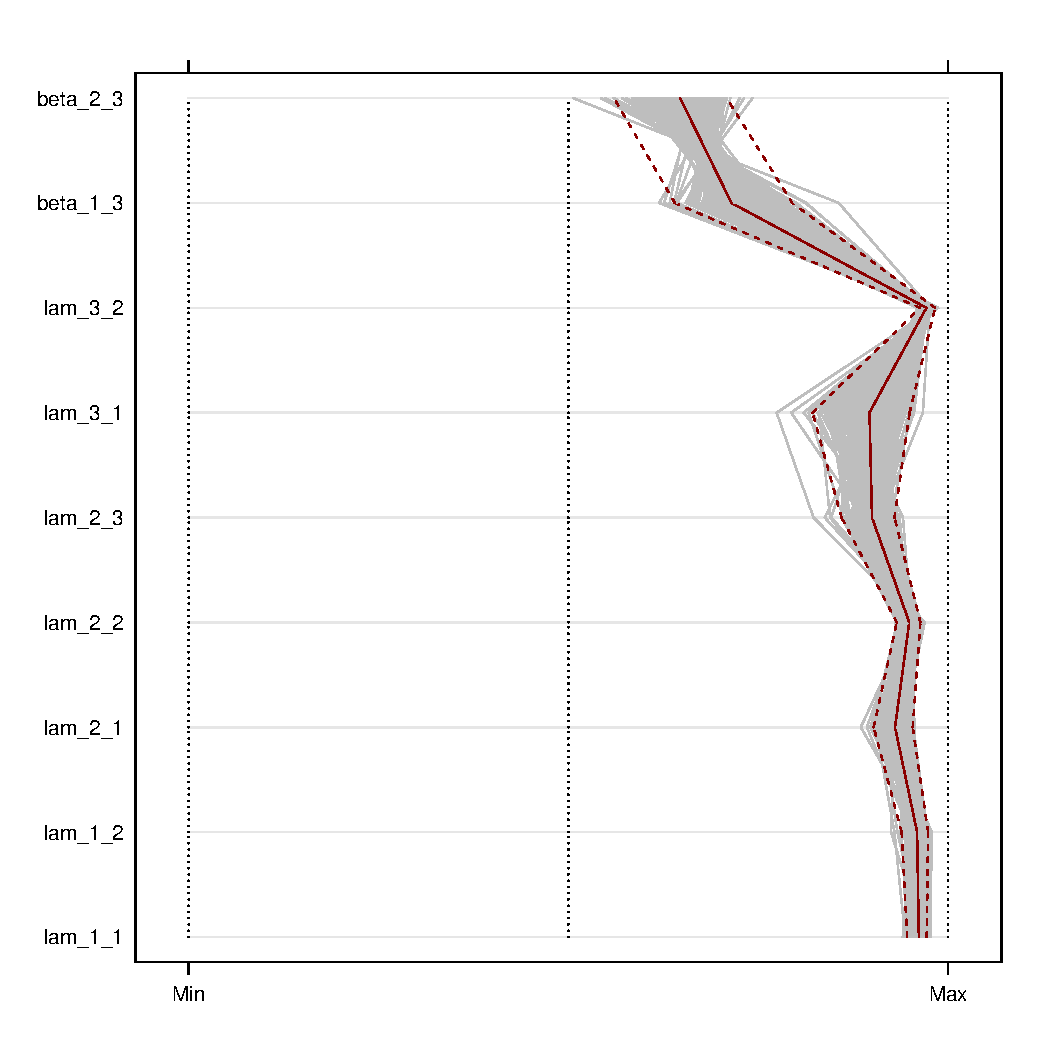
\includegraphics[width=\maxwidth]{figure/boot1} 
\begin{kframe}\begin{alltt}
\hlcom{#plot path coefficients only}
\hlkwd{parallelplot}\hlstd{(new_PB_model_boot,} \hlkwc{pattern}\hlstd{=}\hlstr{"beta"}\hlstd{,} \hlkwc{reflinesAt}\hlstd{=}\hlkwd{c}\hlstd{(}\hlopt{-}\hlnum{1}\hlstd{,}\hlnum{0}\hlstd{,}\hlnum{1}\hlstd{))}
\end{alltt}
\end{kframe}
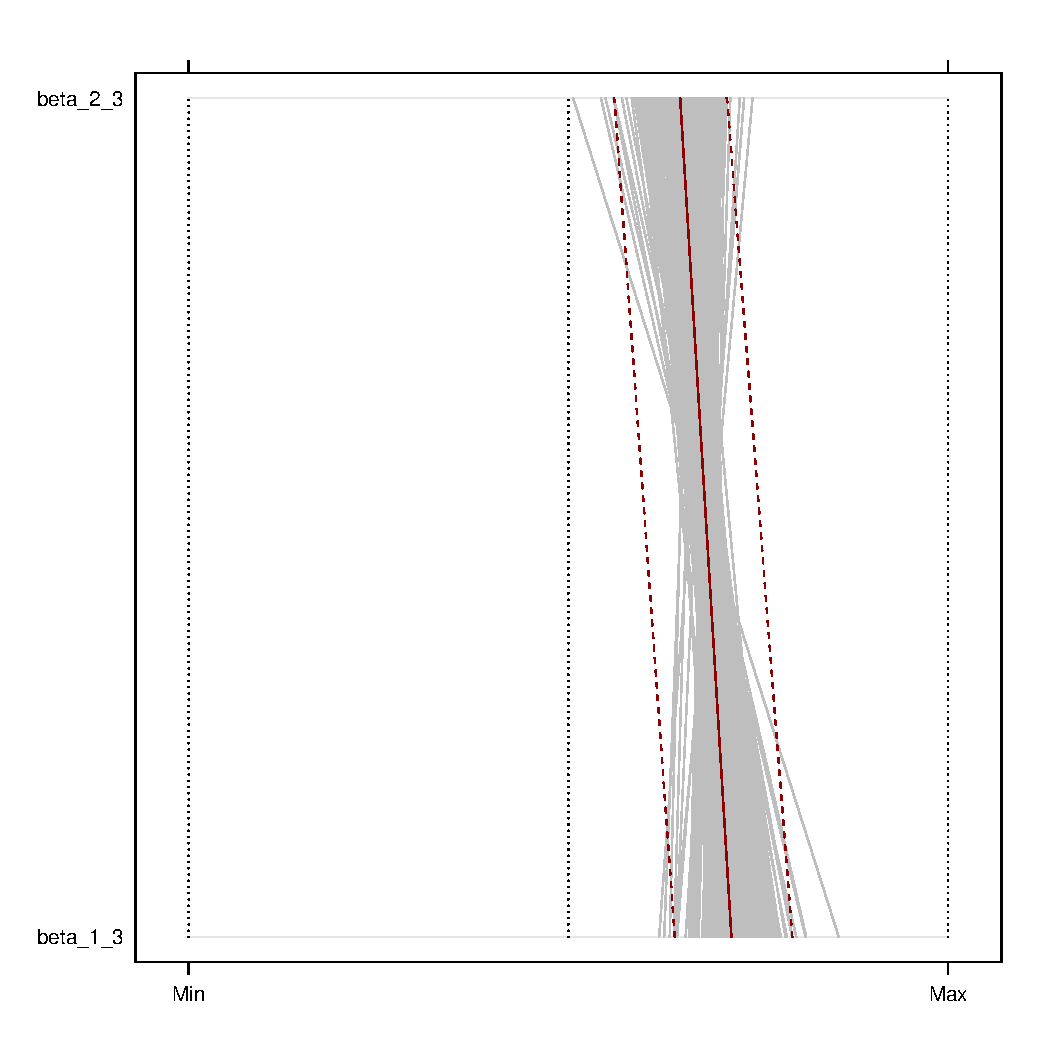
\includegraphics[width=\maxwidth]{figure/boot2} 
\begin{kframe}\begin{alltt}
\hlcom{#plot outer loadings only}
\hlkwd{parallelplot}\hlstd{(new_PB_model_boot,} \hlkwc{pattern}\hlstd{=}\hlstr{"lam"}\hlstd{,}\hlkwc{reflinesAt}\hlstd{=}\hlkwd{c}\hlstd{(}\hlopt{-}\hlnum{1}\hlstd{,}\hlnum{0}\hlstd{,}\hlnum{1}\hlstd{))}
\end{alltt}
\end{kframe}
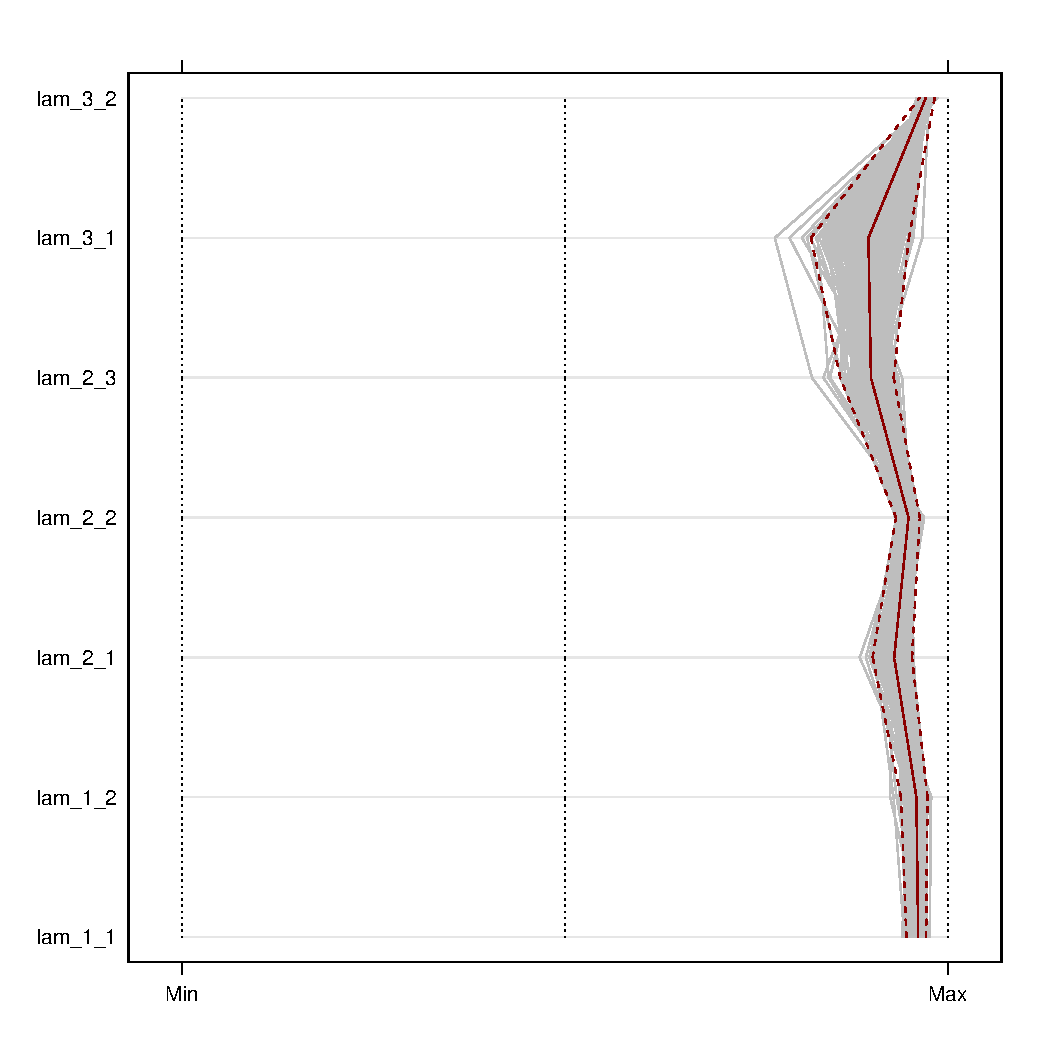
\includegraphics[width=\maxwidth]{figure/boot3} 
\begin{kframe}\begin{alltt}
\hlcom{#plot path coefficients only}
\hlkwd{densityplot}\hlstd{(new_PB_model_boot,} \hlkwc{pattern}\hlstd{=}\hlstr{"beta"}\hlstd{)}
\end{alltt}
\end{kframe}
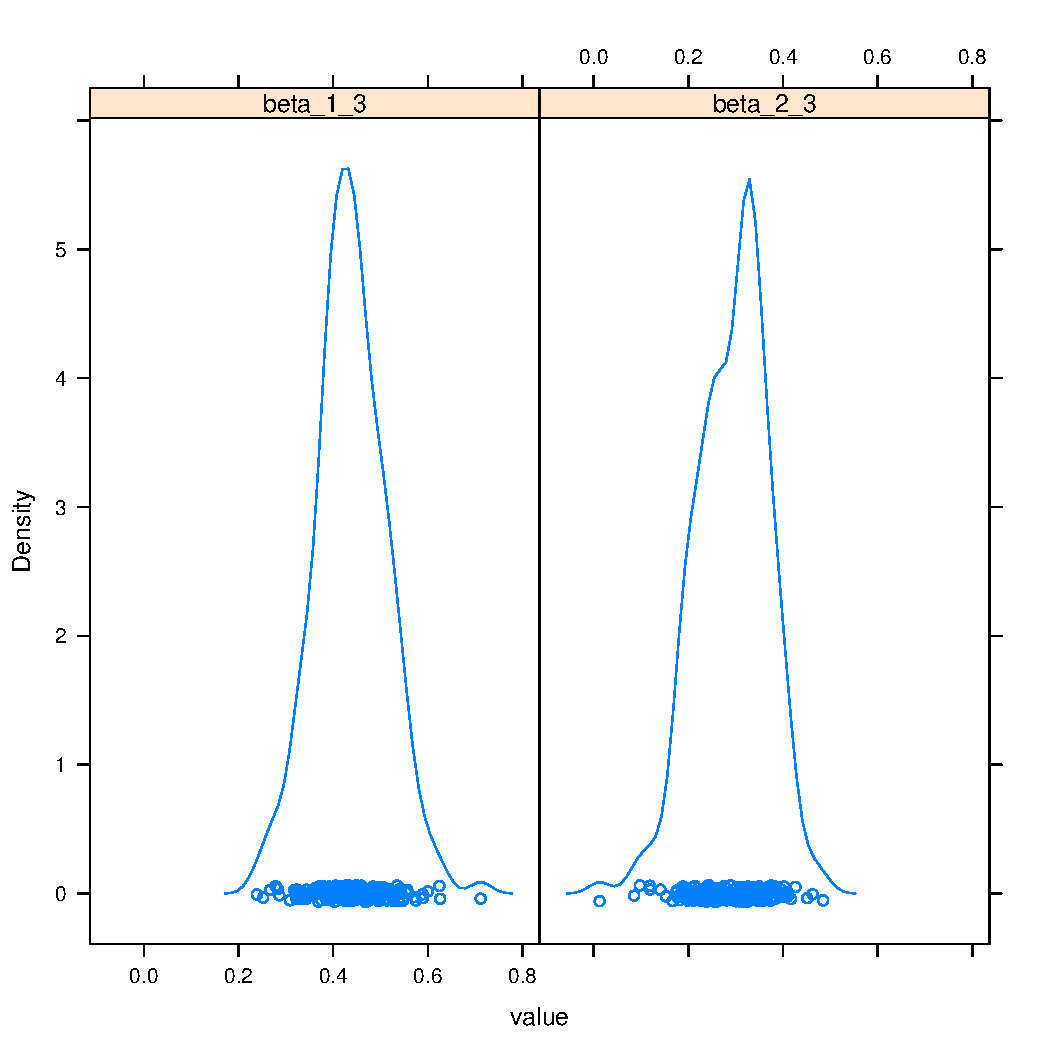
\includegraphics[width=\maxwidth]{figure/boot4} 
\begin{kframe}\begin{alltt}
\hlcom{#plot outer loadings only}
\hlkwd{densityplot}\hlstd{(new_PB_model_boot,} \hlkwc{pattern}\hlstd{=}\hlstr{"lam"}\hlstd{)}
\end{alltt}
\end{kframe}
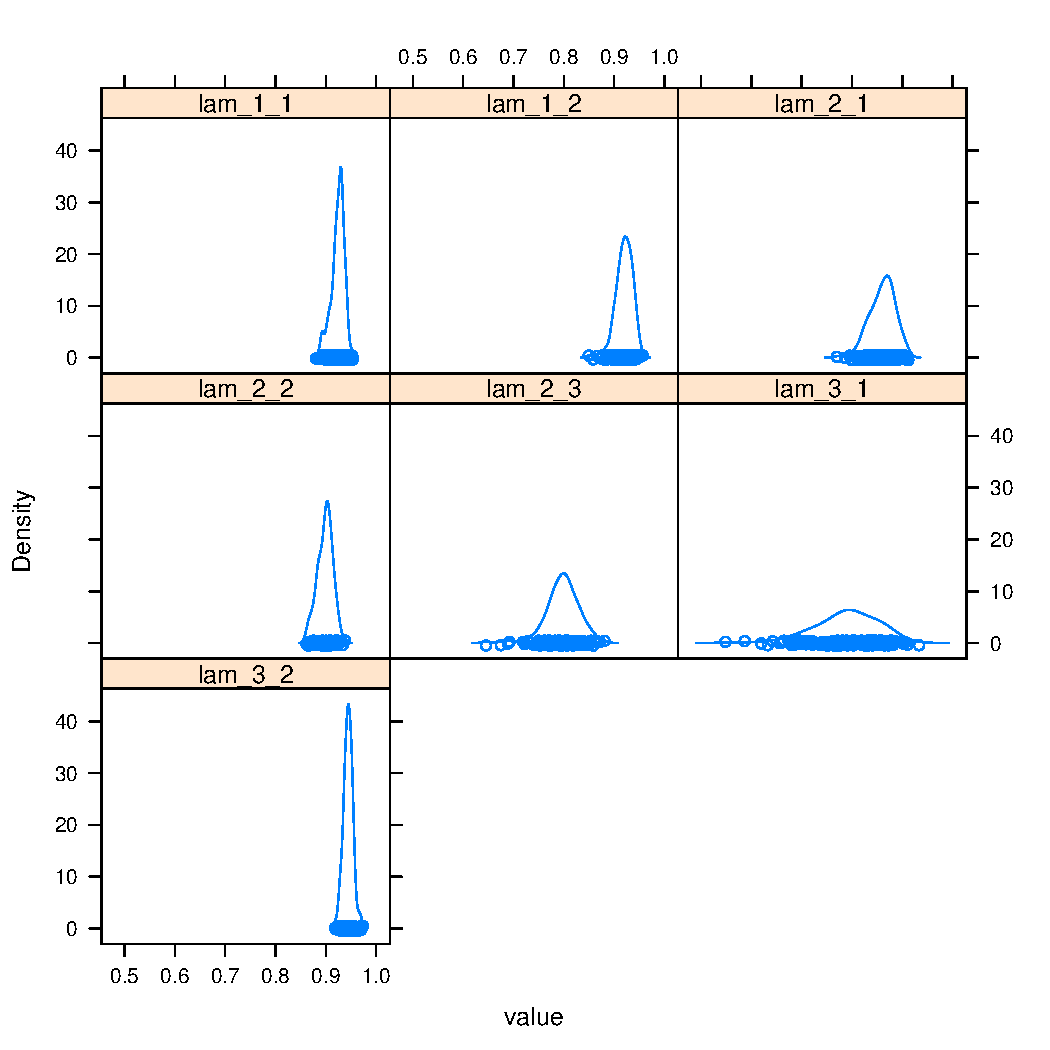
\includegraphics[width=\maxwidth]{figure/boot5} 

\end{knitrout}

Beschreibung zum Code:\\
Zunächst wird ein "seed" erstellt, da beim bootstrapping Verfahren mit jedem erneuten ausführen zufällige unterschiedliche Datensätze (samples) gebildet werden. Mit der Funktion set.seed() kann der Status des Zufallsgenerator gespeichert werden, sodass bei erneutem ausführen der bootsempls() Funktion die gleichen samples und somit auch die gleichen Werte berechnet werden. Die Funktion bootsempls() erhält als Parameter das Modell: new\_PB\_model, die Anzahl der samples: nboot=300 und verbose=TRUE zeigt den Prozess des bootstrapping in der Console an. Nboot, also die Anzahl der Samples sollte mindestens höher als die originale Anzahl der Beobachtungen sein, eine Größe von 5000 wird empfohlen. Die "cases", also die Größe der einzelnen Samples sollte der Anzahl der validen Beobachtungen entsprechen. Dies muss jedoch nicht extra als Parameter an die bootsempls() Methode übergeben werden.\\
Mit new\_PB\_model\_boot wird das erzeugte Objekt ausgegeben. Es enthält die Berechnungen der äußeren Ladungen und Pfadkoeffizienten, sowie den entsprechenden Bias und Standardfehler. Mit dem summary() Befehl wird zusätzlich noch der niedrigste und Höchste Wert angezeigt bei einem Konfidenzintervall von 0.95 (siehe Parameter level=0.95). Dies bedeutet dass die niedrigsten und höchsten Werte nur für das Konfidenzintervall von 95\% gezeigt werden. Es werden also jeweils 2.5\% unten und oben "abgeschnitten", da diese nicht häufig genug vorkommen um repräsentativ zu sein. In der Ausgabe stehen allerdings die Beziehungen nun in einer anderen Notation, wie schon beim Plot des Strukturmodells als Pfadmodell. Durch den Befehl new\_PB\_model\_boot\$fitted\_model\$ können jedoch bequem beide Notationen angezeigt werden und somit "übersetzt" werden.\\
Anschließend werden diese Daten graphisch mit der Funktion parallelplot() dargestellt. Diese erhält als Parameter das neu erstellte Objekt new\_PB\_model\_boot, die Teilmenge new\_PB\_model\_boot\$t und eine refline an der Stelle 0. Die Teilmenge t ist dabei eine Matrix mit den berechneten Werten jeder einzelnen Bootstrap Replikation (Stichprobenziehung, case). Die Referenzlinien bei -1,0,1 dienen lediglich dazu, einschätzen zu können ob die Werte negativ oder positiv sind. Der Plot zeigt die schon erwähnten Pfadkoeffizienten, bzw. äußeren Ladungen aus der t Matrix in visueller Form. Eine graue Linie steht dabei für jeweils eine Stichprobenziehung. Die durchgezogene rote Linie zeigt die usprünglichen "originalen" (ohne Bootstrapping) ermittelten Beziehungen an. Die gestrichelte rote Linie gibt die Werte, welche innerhalb des Konfidenzintervall von 0.95 liegen an. Die gestrichelten vertikalen schwarzen Linien stellen die Referenzlinien bei -1,0,1 dar. Auf der Y-Achse sind die jeweiligen Beziehungen dargestellt und auf der X-Achse die entsprechenden Werte von -1 bis 1. Anschließend kann durch den zusätzlichen Parameter pattern="beta" (pattern="lam") nur die Pfadkoeffizienten (äußeren Ladungen) der Plot auf die jeweilige Beziehung beschränkt werden. Eine weitere Möglichkeit der Visualisierung stellt die densityplot() Funktion dar, welche analog die Ergebnisse in einer Verteilungsfunktion zeigt.\\
Die empirischen t-Werte (Achtung nicht verwechseln mit der oben genannten t Matrix, diese heißt lediglich so) werden nun mit der folgenden Formel ermittelt:
\begin{equation}
t = \frac{p_{ij}}{se^{*}_{p_{ij}}}
\end{equation}
mit:\\
\begin{tabular}{lll}
$t$ &= empirischer t-Wert\\
$p_{ij}$  &= "originaler" Pfadkoeffizient\\
$se^{*}_{p_{ij}}$ &= Bootstrapping Standardfehler\\
\end{tabular}
\\
Der zugehörige R Code sieht wie folt aus:
\begin{knitrout}
\definecolor{shadecolor}{rgb}{0.969, 0.969, 0.969}\color{fgcolor}\begin{kframe}
\begin{alltt}
\hlcom{#store summary in s}
\hlstd{s} \hlkwb{<-} \hlkwd{summary}\hlstd{(new_PB_model_boot)}

\hlcom{#get standard errors}
\hlstd{stderr} \hlkwb{<-} \hlstd{s}\hlopt{$}\hlstd{table}\hlopt{$}\hlstd{Std.Err}

\hlcom{#get original coefficients}
\hlstd{new_PB_model_boot}\hlopt{$}\hlstd{t0}
\end{alltt}
\begin{verbatim}
## [1] 0.9227 0.9180 0.8600 0.8974 0.7993 0.7927 0.9424 0.4292 0.2942
\end{verbatim}
\begin{alltt}
\hlcom{#calculate t-values}
\hlstd{t_values} \hlkwb{<-} \hlstd{new_PB_model_boot}\hlopt{$}\hlstd{t0}\hlopt{/}\hlstd{stderr}

\hlcom{#show t_values}
\hlstd{t_values}
\end{alltt}
\begin{verbatim}
## [1]  70.371  53.261  33.773  59.506  23.084  12.440 101.849   5.752   3.911
\end{verbatim}
\end{kframe}
\end{knitrout}
Zunächst wird ein Vektor mit den Standardfehlern erstellt, welche durch das Speichern des summary() Outputs in der Variable "s" mit dem \$ Operator angesteuert werden können. Die "originalen" Koeffizienten können einfacher durch new\_PB\_model\_boot\$t0 abgerufen werden. Nun wird ein neuer Vektor t\_values durch Division der "originalen" Werte durch die jeweiligen Standardfehler erstellt. Liegt nun ein t-Wert über einem festgelegten kritischen Wert von bspw. 2.57 (Signifikanzniveau = 1\%), ist die korrespondierende Beziehung signifikant mit einer Irrtumswahrscheinlichkeit von 1\%. Das Signifikanzniveau hängt dabei vom Forschungsgebiet ab. Im Marketing ist ein Signifikanzniveau von 5\% üblich, was einem kritischen Wert von 1.96 entspricht. Da jedoch alle ermittelten t-Werte über 4 liegen, erfüllen diese alle gebräuchlichen Signifikanzniveaus und können somit auch als signifikant angesehen werden.\\

\paragraph{Determinationskoeffizient}

Die Kennzahl $R^2$ ist ein Messzahl für den erklärten Anteil der Varianz einer abhängigen Variablen durch ein statistisches Modell. Mögliche Werte gehen von 0 (0\% der Varianz wurden erklärt, kein linearer Zusammenhang) bis 1 (100\% der Varianz wurden erklärt, perfekter linearer Zusammenhang). Vereinfacht bedeutet dies, dass bei einem $R^2$ von 1 alle prognostizierten Werte den tatsächlich gemessenen Werten entsprechen. Da die latente Variable Kundenzufriedenheit in diesem Modell die einzige abhängige (analog: endogene) Variable darstellt, liefert die Methode auch nur für diese einen Wert. Die Funktion rSquared() bekommt als einzigen Parameter das komplette Modell (PB\_model).
\begin{knitrout}
\definecolor{shadecolor}{rgb}{0.969, 0.969, 0.969}\color{fgcolor}\begin{kframe}
\begin{alltt}
\hlkwd{rSquared}\hlstd{(PB_model)}
\end{alltt}
\begin{verbatim}
##                     R-squared
## Performance                 .
## Preis_Leistung              .
## Kundenzufriedenheit      0.42
\end{verbatim}
\begin{alltt}
\hlkwd{rSquared}\hlstd{(new_PB_model)}
\end{alltt}
\begin{verbatim}
##                     R-squared
## Performance                 .
## Preis_Leistung              .
## Kundenzufriedenheit      0.38
\end{verbatim}
\end{kframe}
\end{knitrout}
Allerdings lässt sich laut Backhaus et al.\cite{backhaus2004industriegutermarketing} keine allgemein gültige Aussage formulieren, ab welcher Höhe ein $R^{2}$ als gut zu betrachten ist, da dies von der Problemstellung abhängt. In der Marketing Forschung werden als Daumenregel $R^{2}$ Werte von 0.75, 0.50 und 0.25 als wesentlich, moderat und schwach angesehen.\cite{hair2011pls,henseler2009use} Modelle sollten nicht auf Basis der $R^{2}$ Werte spezifiziert werden, da diese künstlich durch lediglich genügend erklärende Variablen erhöht werden können. Stattdessen sollen die $R^{2}$ Werte zwar hoch sein, jedoch mit einer möglichst geringen Anzahl an erklärende Variablen. Dazu gibt es das korrigierte $R^{2}_{adj}$, welches zusätzlich die Anzahl der exogenen Variablen in der Berechnung berücksichtigt und somit Modelle vergleichbar macht, die mit einer unterschiedlichen Anzahl an erklärenden Variablen einen unterschiedlichen $R^{2}$ Wert erreichen. Da dies jedoch in dem vorgestellten Modell aufgrund der lediglich 2 exogenen Variablen wenig Sinnvoll ist, wird dies hier nur zur Veranschaulichung demonstriert. 
\begin{equation}
 R^{2}_{adj} = 1-(1-R^{2})*\frac{n-1}{n-k-1}
\end{equation}

mit:\\
\begin{tabular}{llll}
$R^{2}_{adj}$ &= korrigiertes $R^{2}$\\
n  &= Zahl der Beobachtungswerte\\
k &= Zahl der erklärenden Variablen\\
n-k-1 &= Zahl der Freiheitsgrade
\end{tabular}
\\
Mit der Zahl der erklärenden Variablen ist jedoch nicht die Gesamtmenge des Modells gemeint, sondern lediglich diese welche die endogene Variable erklären. (Für die $R^{2}$ berechnet wurde)\\
Der korrespondierende R-Code:
\begin{knitrout}
\definecolor{shadecolor}{rgb}{0.969, 0.969, 0.969}\color{fgcolor}\begin{kframe}
\begin{alltt}
\hlcom{#get position of target R^2}
\hlkwd{rSquared}\hlstd{(new_PB_model)}
\end{alltt}
\begin{verbatim}
##                     R-squared
## Performance                 .
## Preis_Leistung              .
## Kundenzufriedenheit      0.38
\end{verbatim}
\begin{alltt}
\hlcom{#position is 3!}

\hlcom{#get total number of complete cases}
\hlstd{new_PB_model}\hlopt{$}\hlstd{N}\hlopt{-}\hlkwd{length}\hlstd{(new_PB_model}\hlopt{$}\hlstd{incomplete)}
\end{alltt}
\begin{verbatim}
## [1] 210
\end{verbatim}
\begin{alltt}
\hlcom{#adjusted rSquared for LV Kundenzufriedenheit}
\hlstd{adjrSquared} \hlkwb{<-} \hlnum{1}\hlopt{-}\hlstd{(}\hlnum{1}\hlopt{-}\hlkwd{rSquared}\hlstd{(new_PB_model)[}\hlnum{3}\hlstd{])}\hlopt{*}\hlstd{((}\hlnum{210}\hlopt{-}\hlnum{1}\hlstd{)}\hlopt{/}\hlstd{(}\hlnum{210}\hlopt{-}\hlnum{2}\hlopt{-}\hlnum{1}\hlstd{))}

\hlcom{#print result}
\hlstd{adjrSquared}
\end{alltt}
\begin{verbatim}
## [1] 0.3738
\end{verbatim}
\end{kframe}
\end{knitrout}
Hier wird nun das korrigierte $R^{2}$ für die endogene latente Variable Kundenzufriedenheit berechnet. Dies geschieht nach der oben vorgestellten Formel. Erwähnenswert ist hier die Nummer 3 in den eckigen Klammern nach der normalen rSquared() Funktion. Diese ist eigentlich nicht notwendig, da lediglich 1 $R^{2}$ berechnet wurde, falls es jedoch mehrere erklärte (endogene) Variablen gibt wird diese wichtig, da mit der oben Vorgestellten Formel nicht ein kompletter Vektor berechnet werden kann wie bei den Standardfehlern. Dies begründet sich dadurch, dass die Zahl (k) der exogenen, also erklärenden Variablen für jede endogene, erklärte Variable unterschiedlich ist. Somit kann mit den eckigen Klammern wie bei einem Array lediglich das $R^{2}$ der Kundenzufriedenheit angesprochen werden. Kundenzufriedenheit hat 2 erklärende Variablen Performance und Preis\_Leistung, daher beträgt k = 2. Nun fehlt nur noch die Zahl der Beobachtungswerte (n) welches mit 210 ausgewiesen ist. Dies kann entweder nach dem durchführen der sempls() Methode in der Console als Output abgelesen werden (Total number of complete cases: 210) oder durch Subtraktion der nicht validen Fälle von der gesamten Fallzahl (N).\\
Beachte jedoch, dass $R^{2}_{adj}$ nicht wie $R^{2}$ interpretiert wird, sondern lediglich zum Vergleich mit anders spezifizierten Modellen herangezogen wird. Zur Veranschaulichung wird erneut ein neues Modell spezifiziert, welches die weiteren exogenen Variablen Ambiente und Kenntnisstand beinhaltet, die beide ebenfalls die Kundenzufriedenheit erklären.
\begin{knitrout}
\definecolor{shadecolor}{rgb}{0.969, 0.969, 0.969}\color{fgcolor}\begin{kframe}
\begin{alltt}
\hlcom{#specify new model}
\hlstd{diff_PB_model} \hlkwb{<-} \hlkwd{sempls}\hlstd{(}\hlkwc{model} \hlstd{=} \hlkwd{plsm}\hlstd{(}\hlkwc{data} \hlstd{= CBdata,}
                        \hlkwc{strucmod} \hlstd{=} \hlkwd{cbind}\hlstd{(}\hlkwd{c}\hlstd{(}\hlstr{"Preis_Leistung"}\hlstd{,}\hlstr{"Performance"}\hlstd{,}
                                           \hlstr{"Ambiente"}\hlstd{,}\hlstr{"Kenntnisstand"}\hlstd{),}
                                         \hlkwd{c}\hlstd{(}\hlkwd{rep}\hlstd{(}\hlstr{"Kundenzufriedenheit"}\hlstd{,}\hlnum{4}\hlstd{))),}
                        \hlkwc{measuremod} \hlstd{=} \hlkwd{cbind}\hlstd{(}\hlkwd{c}\hlstd{(}\hlkwd{rep}\hlstd{(}\hlstr{"Preis_Leistung"}\hlstd{,}\hlnum{3}\hlstd{),}
                                             \hlkwd{rep}\hlstd{(}\hlstr{"Performance"}\hlstd{,}\hlnum{2}\hlstd{),}
                                             \hlkwd{rep}\hlstd{(}\hlstr{"Kundenzufriedenheit"}\hlstd{,}\hlnum{2}\hlstd{),}
                                             \hlstr{"Ambiente"}\hlstd{,}\hlstr{"Kenntnisstand"}\hlstd{),}
                                           \hlkwd{c}\hlstd{(}\hlstr{"SQ009"}\hlstd{,}\hlstr{"SQ076"}\hlstd{,}\hlstr{"SQ092"}\hlstd{,}\hlstr{"SQ079"}\hlstd{,}
                                             \hlstr{"SQ080"}\hlstd{,}\hlstr{"SQ046"}\hlstd{,}\hlstr{"SQ110"}\hlstd{,}\hlstr{"SQ021"}\hlstd{,}\hlstr{"SQ024"}\hlstd{))),}
                        \hlkwc{data} \hlstd{= CBdata)}
\end{alltt}
\begin{verbatim}
## Data rows: 4, 5, 6, 8, 11, 16, 18, 20, 29, 32, 33, 36, 37, 39, 43, 55, 61, 72, 76, 77, 80, 86, 90, 92, 95, 96, 97, 100, 101, 102, 111, 116, 117, 121, 124, 132, 139, 144, 145, 153, 155, 162, 163, 165, 175, 176, 184, 185, 186, 192, 193, 196, 197, 211, 218, 224, 227, 228, 233, 235, 237, 240, 242, 245, 253, 258, 261 
## are not taken into acount, due to missings in the manifest variables.
##  Total number of complete cases: 194 
## Converged after 6 iterations.
## Tolerance: 1e-07
## Scheme: centroid
\end{verbatim}
\begin{alltt}
\hlcom{#show different model}
\hlstd{diff_PB_model}
\end{alltt}
\begin{verbatim}
##                                           Path Estimate
## lam_1_1                      Ambiente -> SQ021     1.00
## lam_2_1                 Kenntnisstand -> SQ024     1.00
## lam_3_1                   Performance -> SQ079     0.92
## lam_3_2                   Performance -> SQ080     0.92
## lam_4_1                Preis_Leistung -> SQ009     0.86
## lam_4_2                Preis_Leistung -> SQ076     0.89
## lam_4_3                Preis_Leistung -> SQ092     0.80
## lam_5_1           Kundenzufriedenheit -> SQ046     0.84
## lam_5_2           Kundenzufriedenheit -> SQ110     0.91
## beta_1_5       Ambiente -> Kundenzufriedenheit     0.14
## beta_2_5  Kenntnisstand -> Kundenzufriedenheit     0.11
## beta_3_5    Performance -> Kundenzufriedenheit     0.45
## beta_4_5 Preis_Leistung -> Kundenzufriedenheit     0.21
\end{verbatim}
\begin{alltt}
\hlcom{#show new R^2}
\hlkwd{rSquared}\hlstd{(diff_PB_model)[}\hlnum{5}\hlstd{]}
\end{alltt}
\begin{verbatim}
## [1] 0.3815
\end{verbatim}
\begin{alltt}
\hlcom{#compare to old R^2}
\hlkwd{rSquared}\hlstd{(new_PB_model)[}\hlnum{3}\hlstd{]}
\end{alltt}
\begin{verbatim}
## [1] 0.3798
\end{verbatim}
\begin{alltt}
\hlcom{#new_adjusted rSquared for LV Kundenzufriedenheit}
\hlstd{new_adjrSquared} \hlkwb{<-} \hlnum{1}\hlopt{-}\hlstd{(}\hlnum{1}\hlopt{-}\hlkwd{rSquared}\hlstd{(diff_PB_model)[}\hlnum{5}\hlstd{])}\hlopt{*}\hlstd{((}\hlnum{210}\hlopt{-}\hlnum{1}\hlstd{)}\hlopt{/}\hlstd{(}\hlnum{210}\hlopt{-}\hlnum{5}\hlopt{-}\hlnum{1}\hlstd{))}

\hlcom{#show new adjusted rSquared}
\hlstd{new_adjrSquared}
\end{alltt}
\begin{verbatim}
## [1] 0.3663
\end{verbatim}
\begin{alltt}
\hlcom{#compare to old adjusted rSquared}
\hlstd{adjrSquared}
\end{alltt}
\begin{verbatim}
## [1] 0.3738
\end{verbatim}
\end{kframe}
\end{knitrout}
Durch die zwei weiteren exogenen latenten Variablen stieg $R^{2}$ von 0.3797589 auf 0.3814821, wird nun jedoch das korrigierte $R^{2}_{adj}$ berechnet sieht man dass das alte mit 0.3737663 besser als das neue Modell mit 0.3663223 ist. Diese Unterschiede sind sehr gering und werden beim Runden der Werte nicht einmal Sichtbar, man könnte dies jedoch auf die Spitze treiben und zum Beispiel 50 exogene Variablen spezifizieren und somit ein höheres $R^{2}$ erzielen, zur Verdeutlichung reichen allerdings auch solche kleine Unterschiede. Generell sollte darauf geachtet werden ein möglichst hohes $R^{2}$ mit möglichst wenigen erklärenden Variablen zu erzielen. Falls zwischen einem höheren $R^{2}$ oder weniger exogenen Variablen entschieden werden muss, bietet das $R^{2}_{adj}$ eine sinnvolle Kennzahl zur Entscheidung.


Zur Validation des Modells sind folgende Funktionen im semPLS Paket implementiert:
\begin{itemize}
\item qSquared()
\item redundancy()
\item gof()
\end{itemize}

Model criteria
coefficients of determination, R 2 values, for each endogenous LV
Stone-Geisser’s Q 2 for assessment of predictive relevance
Dillon-Goldstein’s rho, also referred to as composite reliability
communality indices for reflectively measured LVs with more than one MV
redundancy indices for endogenous LVs
GoF index (geometric mean of average communality and average deter-
mination coefficient




\newpage
\section{Resultate}%Unsere Resultate stehen hier. 
\subsection{Eigenes Modell nach Bukrhardt}



\begin{figure}[h!]
\centering
\hspace*{-4.8cm}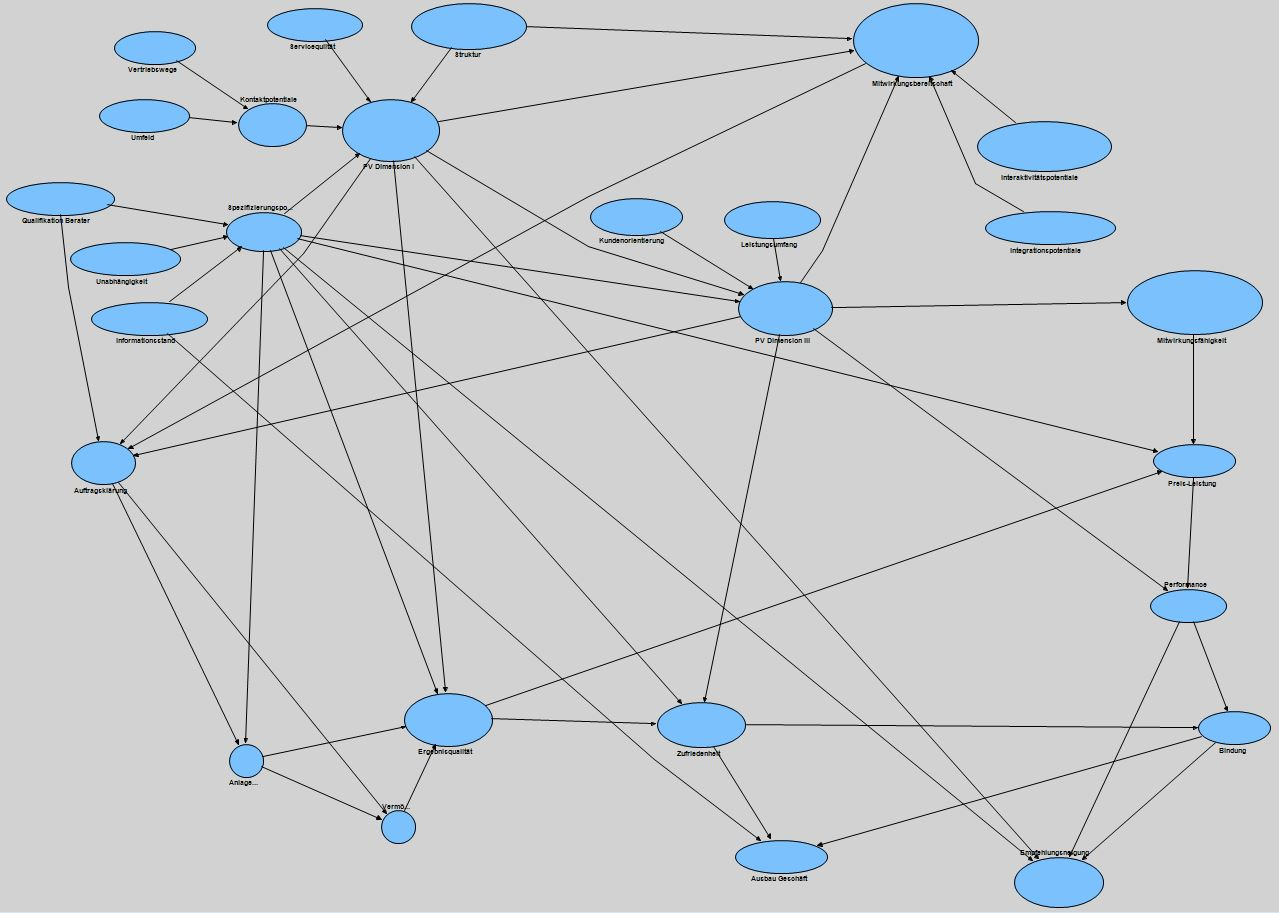
\includegraphics[scale = 0.8]{Grafiken/ausgangsmodell}
\caption{Altes Modell CB EMPF 15}
\label{ausgangsmodell}
\end{figure}

\newpage
Ausgehend von Modell \ref{ausgangsmodell} haben wir uns zunächst intensiv mit dem Fragebogen beschäftigt, um uns einen detaillierten Überblick von der Zuordnung der Konstrukte und der Indikatoren zu verschaffen. Nach ausreichender Einarbeitung in den Themenkomplex haben wir die Konstrukte des Modells überarbeitet und eine neue Zuordnung der Indikatoren vorgenommen. Daraus resultierte das folgende Modell.\\


\begin{figure}[h!]
\centering
\hspace*{-4.8cm}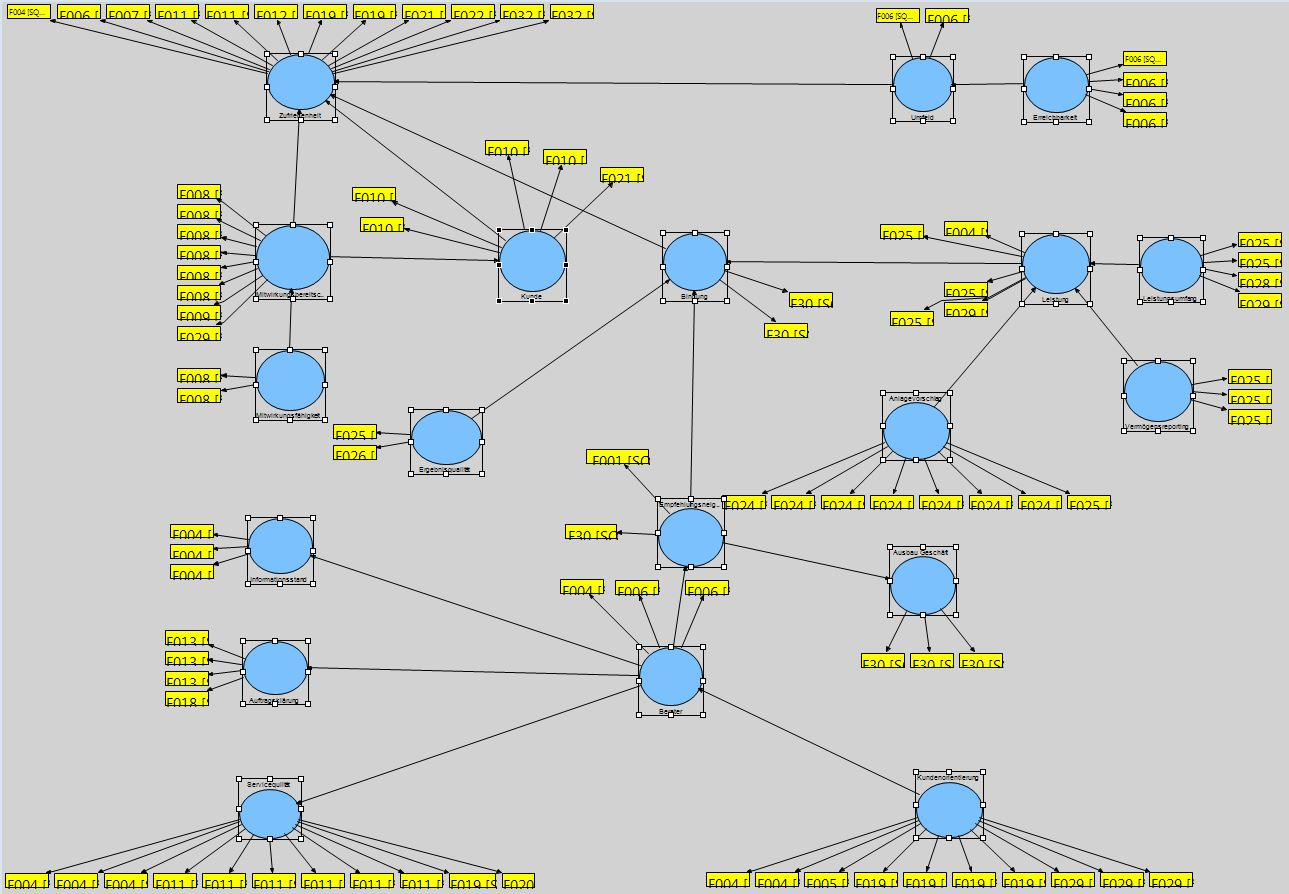
\includegraphics[scale = 0.8]{Grafiken/erstesmodell}
\caption{Altes Modell CB EMPF 15}
\label{erstesmodell}
\end{figure}


%insert LIST here
\newpage
Bei der Berechnung des Modells ist jedoch deutlich geworden, dass das Modell nicht sehr stabil ist. Denn nach erstmaligem Durchlaufen der bootstrapping- Methode erhielten wir sehr gute Werte, als wir jedoch die neuen Werte von Herr Seiler importierten, haben sich diese Werte stark von den zuvor Errechneten unterschieden. Des Weiteren konnten wir den Konstrukten zahlreiche Indikatoren zuordnen, wo jedoch auszuschließen war, dass diese im Zusammenhang mit ihnen standen und trotzdem erhielten wir gute Werte. Aufgrund der Tatsache, dass das Modell sehr komplex und sehr instabil ist, sind Empfehlungen für das Management nicht möglich. Aus diesem Grund haben wir weitere Modelle erstellt und getestet. 

\subsection{Nachbildung Modell Seiler}
Nachdem es uns nicht geglückt ist, die Indikatoren frei nach dem Fragebogen den Konstrukten zuzuordnen, haben wir uns dazu entschieden, das Modell von Seiler nachzubilden. Dazu nahmen wir seine gewählten Konstrukte und versuchten seine Indikatoren mit dem uns vorliegenden Fragebogen abzugleichen. Dabei entstand das folgende Modell.


\hspace*{-4.8cm}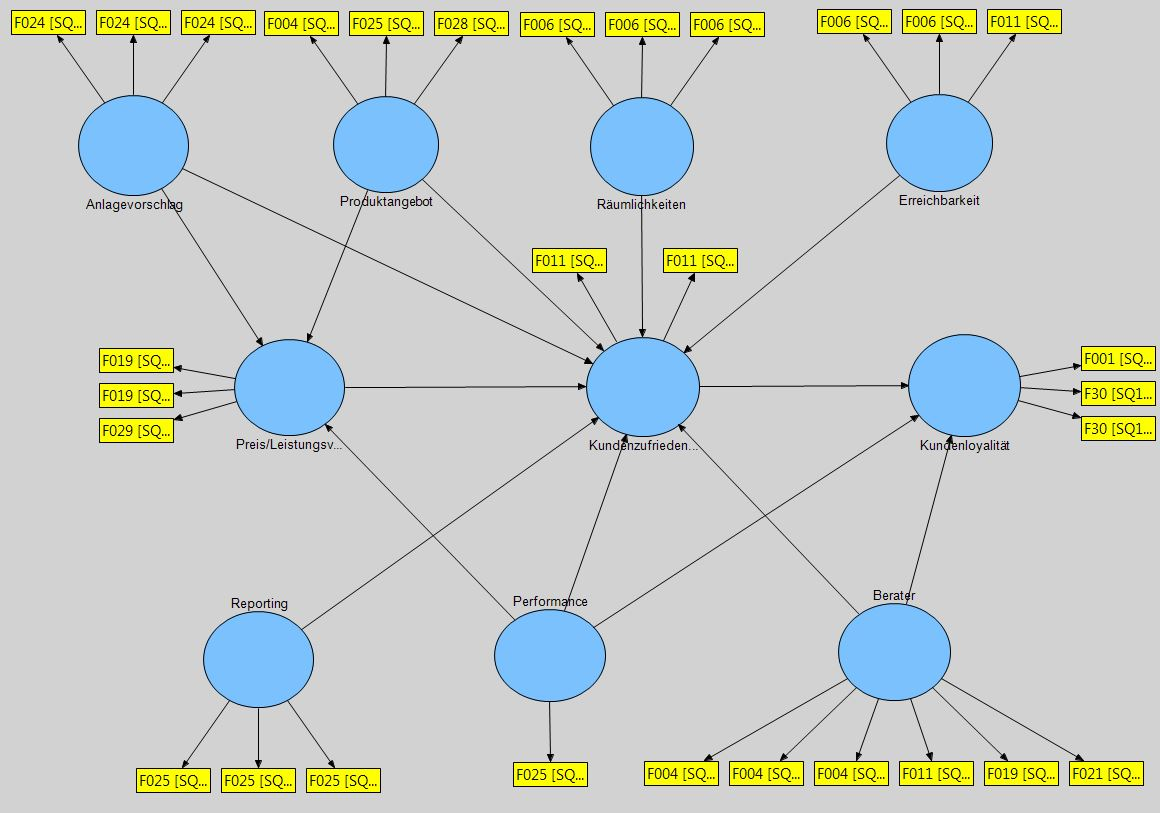
\includegraphics[scale = 0.882]{Grafiken/zweitesmodell}


Bei der Abgleichung der Indikatoren von Seiler mit den Fragen aus unserem Fragebogen gab es nicht immer inhaltliche Übereinstimmungen. Zum besseren Verständnis haben wir unsere Zuweisungen im Folgenden aufgeführt:


%insert LIST here

\subsection{Eigenes Modell nach Seiler}
Bei der Bildung des neuen Strukturmodells haben wir uns primär an Herrn Seiler's Arbeit orientiert. Zu allererst bildeten wir die drei Kernkonstrukte: Bank, Berater und Kunde. Diese beschreiben unseres Erachtens das Grundgerüst unseres Strukturmodells. Aufbauend auf dem Grundgerüst und dem Fragebogen bildeten wir die Konstrukte: Erreichbarkeit, Umgebung, Leistungsumfang, Anlagevorschlag, Vermögensreporting, Mitwirkungsbereitschaft und Mitwirkungsfähigkeit, welche die drei Kernkonstrukte beeinflussen und sich letztendlich auf die Zufriedenheit (Bildung des Konstrukts Zufriedenheit, siehe nächster Abschnitt), unser letztes Konstrukt, übertragen. Anhand der gebildeten Fragebogens fügten wir die dazugehörigen Indikatoren den Konstrukten hinzu.
Dazu wurden die Konstrukte von dem alten Modell am Anfang vereinfacht und zu verschiedenen Konstrukten zusammengefasst. Dafür fügten wir die Konstrukte Empfehlungsneigung, Kundenbindung, Ergebnisqualität sowie Performance und ihre zuvor ermittelten Indikatoren zum Konstrukt Zufriedenheit zu. Wie in Abbildung 1 zu sehen ist, kamen wir zu insgesamt 11 Konstrukten:\\


\hspace*{-4.8cm}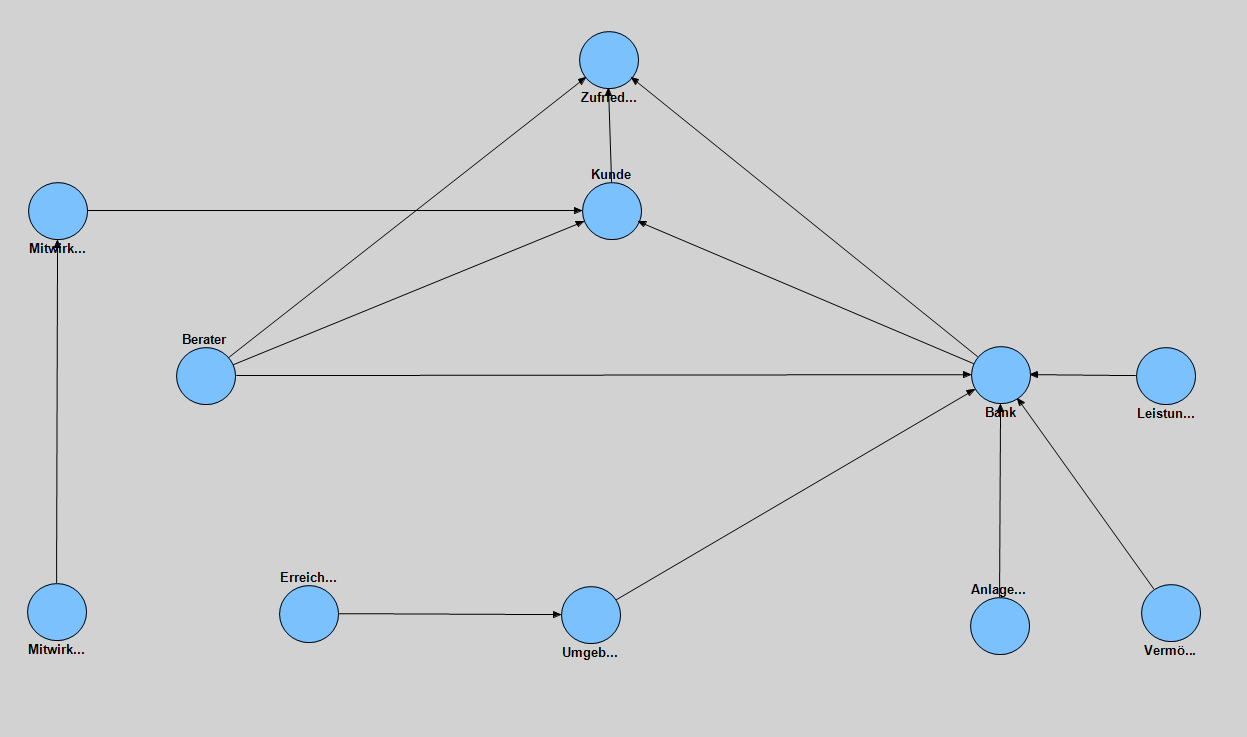
\includegraphics[scale = 0.83]{Grafiken/finalesmodell}


%insert LIST here


\section{Diskussion}%Eine Diskussion über die Resultate findet sich hier.
Nach Aufstellung des Modells muss nun die Bewertung erfolgen. Diese erfolgt in folgenden Schritten:

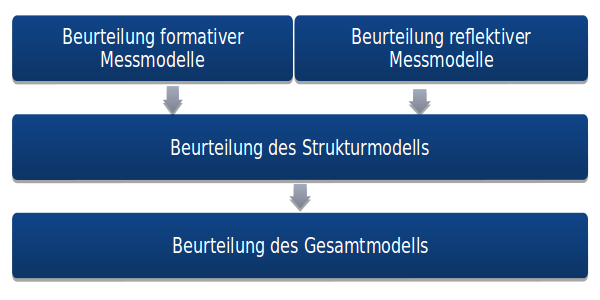
\includegraphics[width = 1\textwidth]{Grafiken/beurteilung}

Wir beurteilen ausschließlich das reflektive Messmodell, da bei unserem Strukturmodell die Richtung der Korrespondenzregeln vom Konstrukt zum Indikator führen, was letztendlich bedeutet, dass die Indikatoren von den Konstrukten beeinflusst werden. Um das reflektive Messmodell zu bewerten, müssen folgende Berechnungen durchgeführt werden: Indikatorreliabilität, Konstruktreliabilität, Durchschnittlich erfasste Varianz sowie die Diskriminanzvalidität.

\section{Ausblick}%Zum Schluss folgt ein Ausblick auf künftige Arbeiten. 




\bibliographystyle{plain} %Stil der Bibliothek
\bibliography{literatur} %Literaturverzeichnis erzeugen

\appendix

\end{document} %Ende des Dokuments
